\documentclass[12pt,oneside]{report}
\usepackage[margin=2.5cm]{geometry}
\linespread{1.375}
\usepackage[utf8]{inputenc}
\usepackage[T1]{fontenc}
\usepackage{polski}
\usepackage{listings}
\usepackage{indentfirst}
\usepackage[shortlabels]{enumitem}
\usepackage{multirow}
\usepackage{makecell}
\usepackage{float}
\usepackage{xcolor}
\usepackage{graphicx}
\usepackage{rotating}
\usepackage{lmodern} %Czcionka
\usepackage{wrapfig} %Tekst wokół obrazu
\raggedbottom %zwalcza dziwne rozciąganie

\definecolor{mygreen}{rgb}{0,0.6,0}
\definecolor{mygray}{rgb}{0.5,0.5,0.5}
\definecolor{mymauve}{rgb}{0.58,0,0.82}

\lstset{ 
	language=[Sharp]C,
	backgroundcolor=\color{white},   % choose the background color; you must add \usepackage{color} or \usepackage{xcolor}; should come as last argument
	basicstyle=\footnotesize,        % the size of the fonts that are used for the code
	breakatwhitespace=false,         % sets if automatic breaks should only happen at whitespace
	breaklines=true,                 % sets automatic line breaking
	captionpos=b,                    % sets the caption-position to bottom
	commentstyle=\color{mygreen},    % comment style
	deletekeywords={...},            % if you want to delete keywords from the given language
	escapeinside={\%*}{*)},          % if you want to add LaTeX within your code
	extendedchars=true,              % lets you use non-ASCII characters; for 8-bits encodings only, does not work with UTF-8
	firstnumber=1,                % start line enumeration with line 1000
	frame=single,	                   % adds a frame around the code
	keepspaces=true,                 % keeps spaces in text, useful for keeping indentation of code (possibly needs columns=flexible)
	keywordstyle=\color{blue},       % keyword style
	numbers=left,                    % where to put the line-numbers; possible values are (none, left, right)
	numbersep=5pt,                   % how far the line-numbers are from the code
	numberstyle=\tiny\color{mygray}, % the style that is used for the line-numbers
	rulecolor=\color{black},         % if not set, the frame-color may be changed on line-breaks within not-black text (e.g. comments (green here))
	showspaces=false,                % show spaces everywhere adding particular underscores; it overrides 'showstringspaces'
	showstringspaces=false,          % underline spaces within strings only
	showtabs=false,                  % show tabs within strings adding particular underscores
	stepnumber=2,                    % the step between two line-numbers. If it's 1, each line will be numbered
	stringstyle=\color{mymauve},     % string literal style
	tabsize=2,	                   % sets default tabsize to 2 spaces
	title=\lstname                   % show the filename of files included with \lstinputlisting; also try caption instead of title
}
\begin{document}
	\begin{titlepage}
		
		\begin{center}
			\begin{figure}[t]
				\centering
				
\includegraphics[width=4.5cm,height=4.5cm]{LogoUO.jpg}
			\end{figure}
		\end{center}
		
		\begin{center}
			{\LARGE  \bf \textsc{UNIWERSYTET OPOLSKI}}
		\end{center}
		\vspace{0.2cm}
		\begin{center}
			{\large \textsc{Wydział Matematyki, Fizyki i Informatyki}}
		\end{center}
		%\vspace{0.2cm}
		\begin{center}
			{\Large \textsc{Instytut Informatyki}}
		\end{center}
		\vspace{0.5cm}
		\begin{center}
			\large    \textsc{Praca iżynierska}
		\end{center}
		\vspace{0.4cm}
		\begin{center}
			\large \textbf{Natalia Szymczak}
		\end{center}
		
		\vspace{0.4cm}
		\begin{center}
			\Large     \textbf{Aplikacja bazodanowa dla klubów jeździeckich}
		\end{center}
		\vspace{0.1cm}
		
		\begin{center}
			\large     \textsc{}
		\end{center}
		\vspace{1.3cm}
		
		\begin{flushright}
			{\large Praca wykonana pod kierunkiem\bigskip
				
				{\bf }} 
			dra Jacka Iwańskiego
		\end{flushright}
		\vspace{0.7cm}
		\begin{center}
			{\large OPOLE 2024}
		\end{center}
	\end{titlepage}

	\thispagestyle{empty}
	\mbox{}
	
	\begin{quote}{\small 
			\noindent
			
			\bigskip
			\noindent
			\textbf{Streszczenie:} 
			
			
			\noindent
			\newline
			\textbf{}
			\vspace{5pt}
			
			\noindent
			\newline
			\textbf{Abstract:} 
			\vspace{5pt}
			
			\vspace{5pt}
			\noindent
			\newline
			\textbf{Keywords:} 
			\vspace{5pt}
			\bigskip
			
			\noindent 
			\textbf{Klasyfikacja tematyczna wg  MSC 2020:}}
	\end{quote}

	\mbox{}
	
	\pagestyle{plain}
	\tableofcontents
	\thispagestyle{empty}
	
	
	\newpage
	\setcounter{page}{1}
	\newpage
\chapter{Wstęp}
\chapter{Przegląd istniejących rozwiązań}
\section{Ridely}
\begin{wrapfigure}{r}{0.65\textwidth}
	\centering
	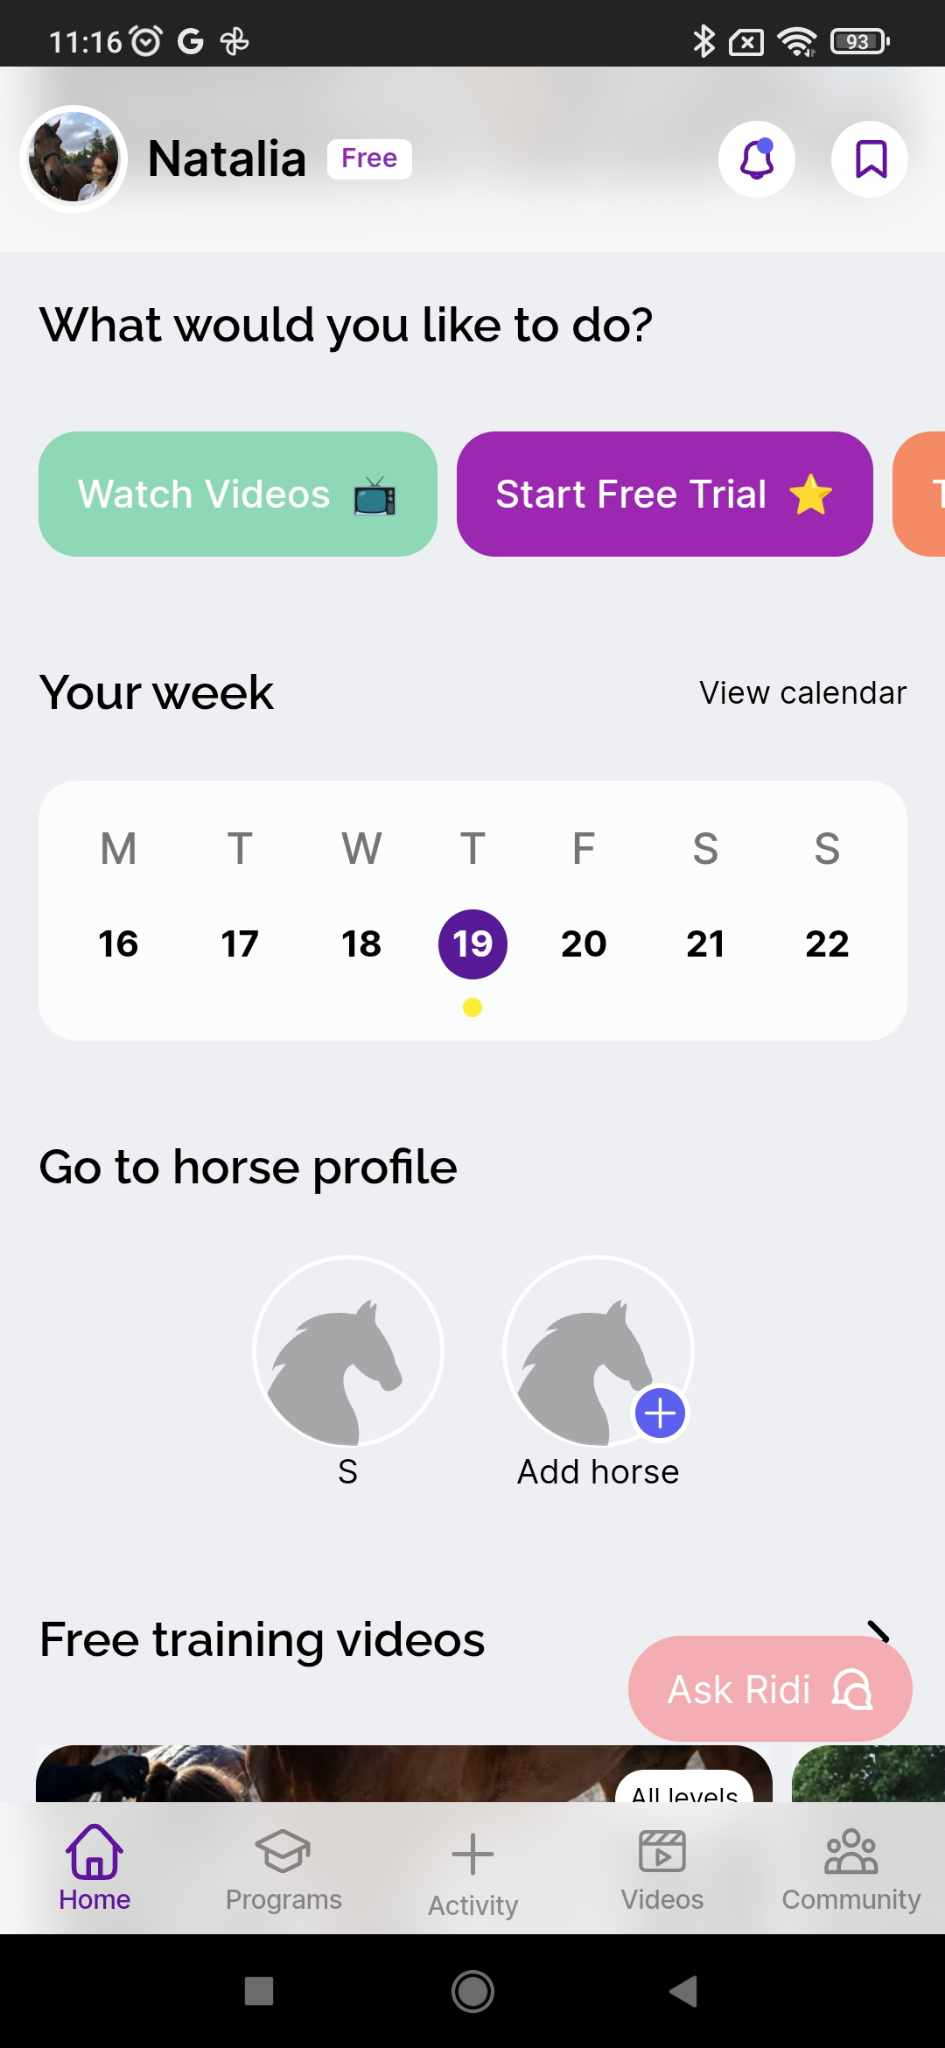
\includegraphics[scale=0.15]{ridely4}
	\caption{Widok główny aplikacji}
	\textit{Źródło opracowanie własne}
	\label{RidelyKalendarz}
\end{wrapfigure}
Ridely to aplikacja pozwalająca na monitorowanie treningów. Dzięki niej możemy zapisać swoje treningi, oglądać poradniki i poprawiać swoje umiejętności jeździeckie. 
Aplikacja ma wiele mocnych stron. Skupia się głównie na monitorowaniu treningów i ten aspekt ma dopracowany bardzo dobrze. O samych aktywnościach można zbierać bardzo dużo informacji, jak także śledzić trening na bieżąco. Jednakże ma także wady. Kalendarz, w którym zaznaczone są aktywności jest mało czytelny i na pierwszy rzut oka nie widzimy co koń robił w poprzednie dni (patrz. rys. \ref{RidelyKalendarz}).
Z zalet można wymienić jeszcze dostępność wielu materiałów wideo pozwalających na doszkolenie się jednakże materiały te są jedynie w języku angielskim. Porównując do stworzonej aplikacji nie ma możliwości zapisu wizyt lekarzy, planów żywienia ani nie ma informacji o zawodach. Jest ona mniej kompleksowa i przez dużą zawartość plików jest dość spora i wolno działa. 
\section{Equilab}
\begin{wrapfigure}{r}{0.65\textwidth}
	\centering
	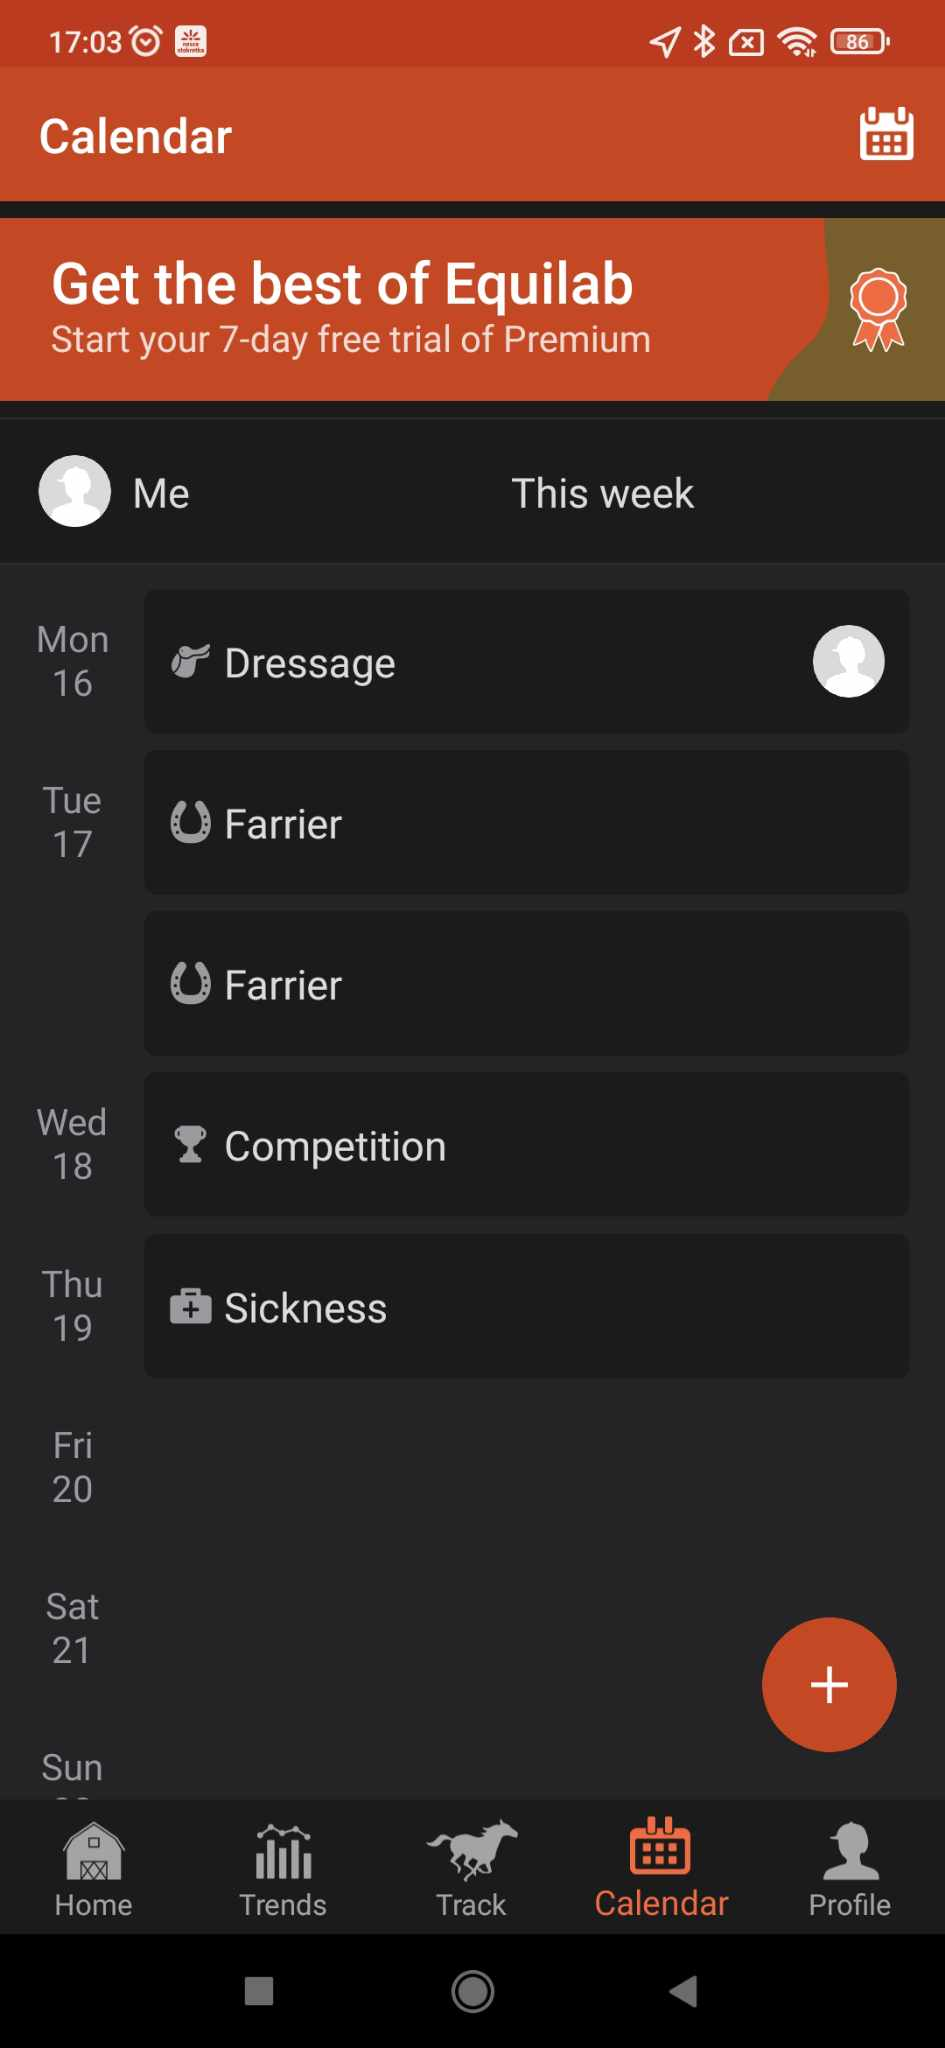
\includegraphics[scale=0.15]{equilab1}
	\caption{Widok kalendarza aplikacji}
	\textit{Źródło opracowanie własne}
	\label{Equilab}
\end{wrapfigure}
Equilab także skupia się głównie na treningach. Nie ma na nim dostępnych materiałów wideo ani pouczających wpisów. Interfejs graficzny jest w miarę przyjazdy użytkownikowi, a sama aplikacja działa płynnie. Dzięki tej aplikacji można śledzić treningi i zapisywać ich trasy. Zapisywanie aktywności obejmuje także podstawowe wizyty lekarskie oraz kowali. Jednakże nie można o nich zapisać wielu informacji. Z minusów aplikacji można także wymienić mało przyjazdy UI w kalendarzu z zapisanymi aktywnościami. W porównaniu do stworzonej aplikacji nie ma możliwości zapisu planów żywienia. Minusem jest także połączenie w jednym widoku aktywności oraz wizyt przez co mamy mniej widocznych informacji i łatwiej się wśród nich zgubić (patrz rys. \ref{Equilab}). W odróżnieniu od naszej aplikacji można tutaj zawierać przyjaźnie między użytkownikami i brać udział w wyzwaniach. Jednakże nie ma kluczowej funkcji udostępniania koni, która po rozmowach z osobami ze środowiska okazała się kluczowa.
\section{Happie Horse}
\begin{wrapfigure}{r}{0.65\textwidth}
	\centering
	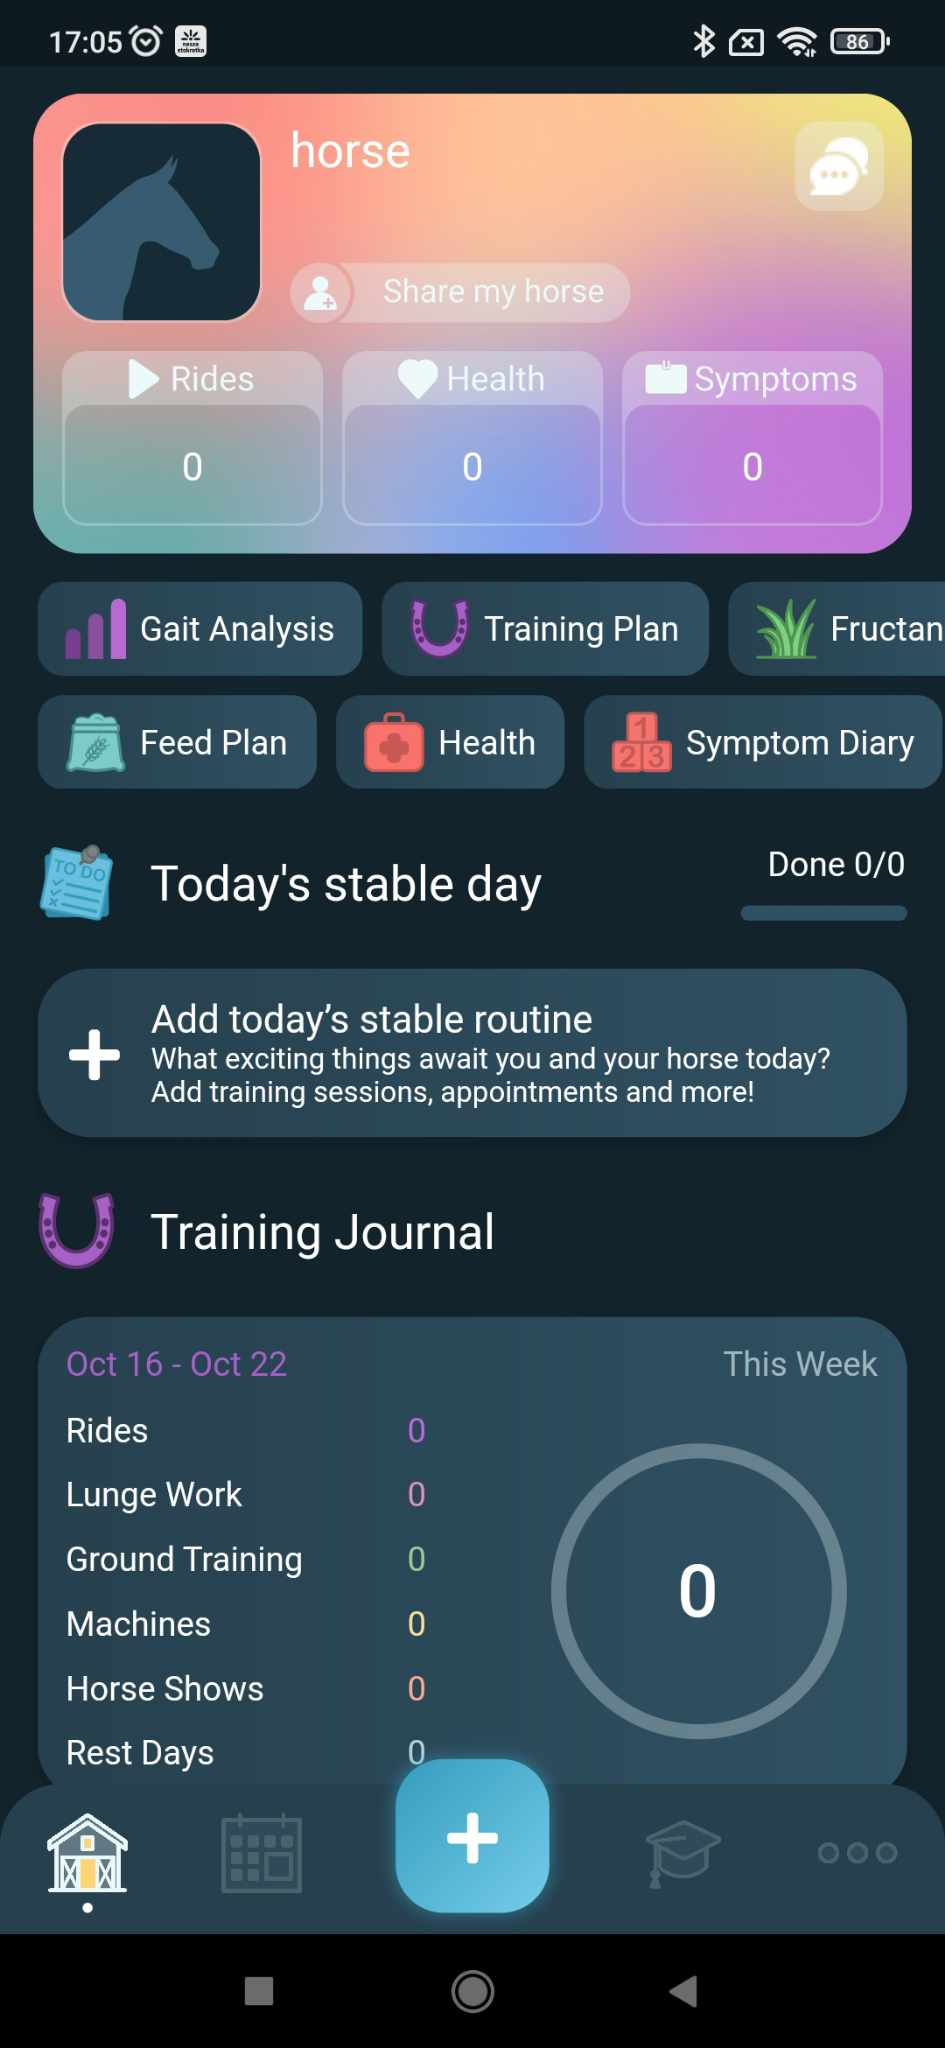
\includegraphics[scale=0.15]{happieHorse1}
	\caption{Widok kalendarza aplikacji}
	\textit{Źródło opracowanie własne}
	\label{HappieHorse}
\end{wrapfigure}
Aplikacja Happie Horse posiada podobne funkcje do zaprojektowanego systemu. Na głównej stronie aplikacji mamy aktywności plan żywienia oraz wizyty u kowali i lekarzy. Aplikacja ma przyjazny chodź dość ciemny interfejs. Zapis aktywności podobnie jak w poprzednich aplikacjach jest mało czytelny i na pierwszy rzut oka nie widać co koń robił przez ostatnie dni. Nie dostępne są także statystki aktywności. W zamian za to aplikacja ma szereg kursów pozwalających na poprawę swoich umiejętności. To czego brakuje tej aplikacji to także funkcja udostępniania koni pomagająca kontrolować swoje konie w trakcie wyjazdów.
\chapter{Technologie użyte w pracy}
\section{Microsoft Visual Studio 2022}
\textcolor{red} {Microsoft Visual Studio to środowisko IDE, za pomocą którego można edytować, debugować jak także kompilować kod. Po stworzeniu aplikacji można ja także opublikować w prost ze środowiska. Środowisko to zawiera wiele funkcji wzbogacających proces tworzenia takich jak narzędzia uzupełniania kodu (Intellisense). Dzięki temu środowisku możemy programować aplikacje na dowolną platformę oraz dowolne urządzenia. }
\section{Microsoft SQL Server 2019 Express}
\textcolor{red} {Microsoft SQL Server jest to system, wspomagający zarządzanie bazą danych stworzony oraz utrzymywany przez firmę Microsoft. MS SQL wykorzystuje język zapytań Transact-SQL, który jest rozwinięciem standardu języka zapytań ANSI/SQL.}

\section{Microsoft SQL Server Management Studio}

\section{Structured Query Language}
\textcolor{red} {SQL czyli Structured Query Language jest to język zapytań wykorzystywany w relacyjnych bazach danych. Umożliwia on tworzenie, modyfikowania oraz zarządzanie bazami danych. Dodatkowo dzięki SQL jesteśmy w stanie pobierać, dodawać, aktualizować oraz usuwać dane znajdujące się w naszej bazie danych. SQL wspiera również tworzenie skomplikowanych zapytań, dzięki czemu możemy wykonywać różne operacje na danych takie jak: filtrowanie, sortowanie, grupowanie oraz łączenie.}

\section{Windows Presentation Foundation}
WPF - Windows Presentation Foundation, jest technologią opracowaną przez Microsoft. Służy ona do tworzenia aplikacji desktopowych na system Windows. Jest częścią .NET Framework i zapewnia on możliwość tworzenia zaawansowanych interfejsów użytkownika wykorzystując język XAML. Interfejs ten jest niezależny od rozdzielczości oraz używa aparatu renderowania opartego na wektorach, aby korzystać z nowoczesnego sprzętu graficznego. WPF dostarcza kontrolki, powiązanie danych, układ, grafike 2D i 3D, animację, style, szablony, dokumenty, multimedia, tekst i typografię, jak także inne elementy interfejsu API platformy .NET. \cite{WPF}

\section{Xamarin}
Xamarin jest to platforma do tworzenia aplikacji mobilnych za pomocą platformy .NET, która automatycznie obsługuje odzyskiwanie i alokowanie pamięci, jak także współdziałanie z platformami bazowymi. Dzięki Xamarinowi możemy pisać aplikacje na androida, iOS jak także na windows phone. Tworzy on warstwę abstrakcji komunikującą się za pomiędzy kodem aplikacji, a kodem bazowej platformy. Aplikacje wykorzystujące Xamarin możemy pisać nie tylko na komputerach PC z systemem Windows lub Linux, lecz także na urządzeniach z systemem MacOS. Architektura systemu Xamarin przedstawiona zostala na rysunku \ref{XamarinArchitecture}. Możemy na nim zobaczyć część architektury dotyczącą platformy android jak także, część dotyczącą platformy iOS.\cite{XamarinLearn}
\begin{figure}[H]
	\centering
	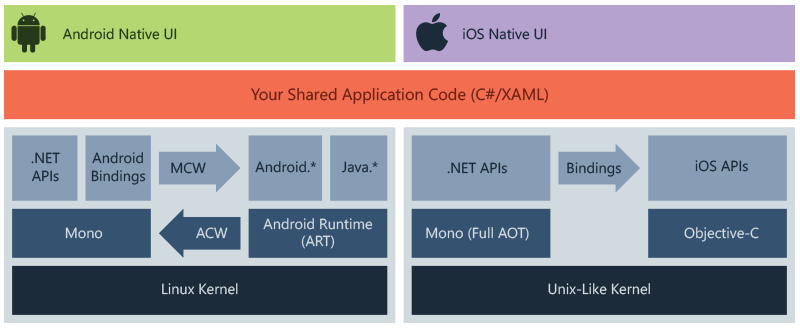
\includegraphics[scale=0.5]{xamarinArchitecture}
	\caption{Architektura platformy Xamarin}
	\textit{Źródło: \cite{XamarinLearn}}
	\label{XamarinArchitecture}
\end{figure}
\subsection{Xamarin.Android}
Aplikacja HorseTracking dostępna będzie jedynie na platformę android. Aby dostosować ją do systemu iOS niezbędne było by urządzenie z systemem MacOS co nie było możliwe.
Xamarin.Android kompilowany jest z języka C\#, do języka pośredniego "just in time", często nazywanego JIT od pierwszych liter nazwy. JIT jest skompilowany do zestawu natywnego po uruchomieniu aplikacji. Xamarin.Android jest uruchamiany w środowisku mono obok maszyny wirtualnej środowiska Android Runtime. Dzięki platformie Xamarin możemy powiązać platformę .Net z przestrzeniami nazw Android.* i Java.*. Za pośrednictwem zarządzanych otok wywoływanych MCW środowisko mono może wywoływać przestrzenie nazw oraz udostępniać otoki wywoływane przez system Android(ACW). Dzięki temu oba środowiska mogą wywoływać kod nawzajem. Na rysunku \ref{AndroidArchitecture} przedstawiona została architektura systemu Xamarin.Android\cite{XamarinLearn}.
\begin{figure}[H]
	\centering
	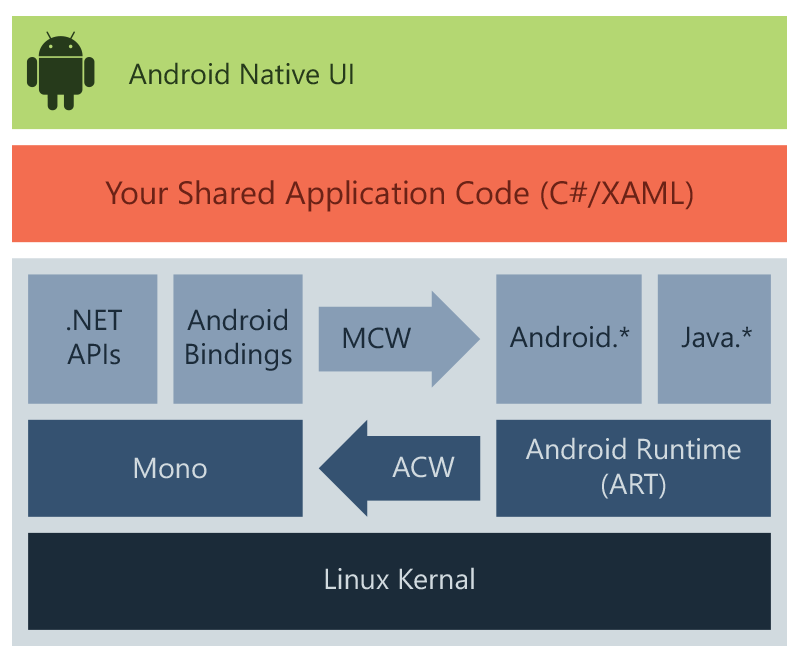
\includegraphics[scale=0.3]{androidArchitecture}
	\caption{Architektura platformy Xamarin.Android}
	\textit{Źródło: \cite{XamarinLearn}}
	\label{AndroidArchitecture}
\end{figure}

\section{Android Device Menager}
{\color{red} Dopisać }
\section{NuGet}
NuGet (logo systemu na rysunku \ref{nugetLogo})jest to mechanizm udostępniania kodu obsługiwany przez firmę Microsoft. 
\begin{figure}[H]
	\centering
	
\includegraphics[scale=0.25]{nugetLogo}
	\caption{Logo systemu NuGet}
	\textit{Źródło: \cite{Nuget}}
	\label{nugetLogo}
\end{figure}
Służy on do współdzielenia kodu. Pakiet NuGet obsługuje hosty prywatne oraz publicznego hosta. Na hoście publicznym NuGet ma tysiące unikatowych pakietów dostępnych dla użytkowników .Net. Niezależnie od tego czy host jest prywatny czy publiczny jest on połączeniem między twórcami pakietów a ich konsumentami. Przepływ informacji między deweloperami pakietów, a ich konsumerami możemy zaobserwować na rysunku \ref{NugetFlow}.
\begin{figure}[H]
	\centering
	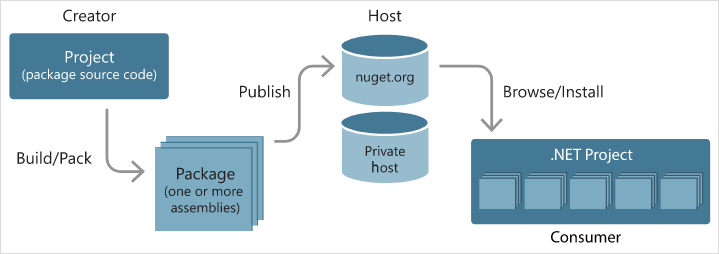
\includegraphics[scale=0.75]{nugetFlow}
	\caption{Przepływ informacji}
	\textit{Źródło: \cite{Nuget}}
	\label{NugetFlow}
\end{figure}
\section{Git, Github, Sourcetree}
Git (logo na rysunku \ref{GitLogo}) to darmowy rozproszony system kontroli wersji typu open source. Zaprojektowany został do obsługi małych oraz bardzo dużych projektów. Dzięki niemu możliwe jest tworzenie backupów oraz zarządzanie nimi. Jak także rozwijanie aplikacji w wiele osób jednocześnie.\cite{git}
\begin{figure}[H]
	\centering
	\includegraphics[scale=0.6]{git}
	\caption{Logo git}
	\textit{Źródło: \cite{git}}
	\label{GitLogo}
\end{figure}
Github (logo na rysunku \ref{GithubLogo}) jest to nakładka na git, dzięki której w łatwiejszy sposób możemy zakładać repozytorium oraz zarządzać kodem.\cite{github}
\begin{figure}[H]
	\centering
	\includegraphics[scale=0.3]{githubLogo}
	\caption{Logo github}
	\textit{Źródło: \cite{github}}
	\label{GithubLogo}
\end{figure}
Sourcetree (logo na rysunku \ref{SourcetreeLogo}) to także nakładka na git, która pozwala na łatwiejsze tworzenie branchy, stashów, oraz szybkie przełączaniem się między gałęziami. Dzięki niemu możemy zarządzać branchami z wielu projektów na raz w sposób przyjaźniejszy niż przez Visual Studio.\cite{sourcetree}
\begin{figure}[H]
	\centering
	
\includegraphics[scale=0.3]{sourcetree}
	\caption{Logo sourcetree}
	\textit{Źródło: \cite{sourcetree}}
	\label{SourcetreeLogo}
\end{figure}
\section{Figma}
Figma jest to narzędzie do projektowania i prototypowania interfejsów aplikacji. Dzięki narzędziom takim jak figma możemy zaplanować cały interfejs jeszcze przed jego implementacją.  Stworzony w ten sposób interfejs możemy przetestować dzięki funkcji prototypowania. Jeszcze przed implementacją może on zostać udostępniony kilku osobą w celu sprawdzenia czy wszystkie funkcje aplikacji są dla użytkownika jasne i intuicyjne. Dzięki temu implementować będziemy interfejs już sprawdzony, więc będzie wymagał on mniej poprawek.
\begin{figure}[H]
	\centering
	\includegraphics[scale=0.10]{FigmaLogo}
	\caption{Logo Figmy}
	\textit{Źródło: \cite{FigmaIcon}}
	\label{FigmaLogo}
\end{figure}
\section{Entity Framework}
Entity Framework to narzędzie do mapowania obiektowo-relacyjnego, który umożliwia tworzenie przejrzystej, przenośnej i wysokopoziomowej warstwy dostępu do danych za pomocą platformy .NET (C\#) dla wielu baz danych.  Pozwala on na wykonywanie podstawowych operacji takich jak dodawanie, pobieranie, uaktualnianie i usuwanie danych. Możemy dzięki niemu także łatwiej zarządzać relacjami w bazie. Zasada działania tego narzędzia przedstawiona została na rysunku \ref{EntityArchitecture}
\begin{figure}[H]
	\centering
	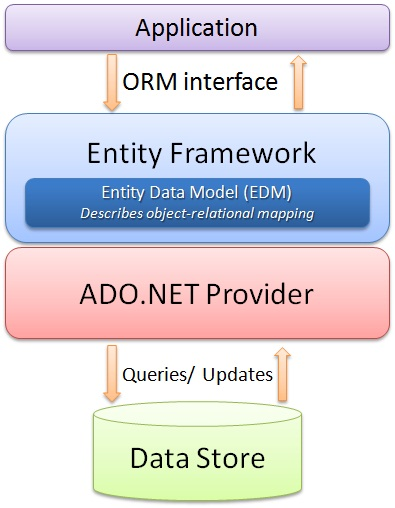
\includegraphics[scale=0.5]{EntityArchitecture}
	\caption{przepływ informacji}
	\textit{Źródło: \cite{Entity}}
	\label{EntityArchitecture}
\end{figure}
{\color{red}
\section{LiveChartsCore}
LiveChartsCore to nugget pozwalający na łatwe i szybkie tworzenie wykresów.
\section{ZXing}
\section{MVVM Toolkit}

\section{Xamarin Community Toolkit}

\section{ZXing.Net.Mobile.Forms}

\section{Xamarin.Essentials}
\section{Microsoft.Extensions.DependencyInjection}}


\chapter{Specyfikacja wymagań}
\section{Opis wycinka rzeczywistości}
Aplikacja przeznaczona jest dla klubów jeździeckich, czyli organizacji zrzeszających jeźdźców startujących w danej dziedzinie sportów konnych. Aplikacja skierowana jest do klubów, których zawodnicy startują w takich dziedzinach jak:
\begin{itemize}
	\item Skoki przez przeszkody,
	\item WKKW (skrót od ,,Wszechstronny konkurs konia wierzchowego''),
	\item Ujeżdżenie.
\end{itemize}

W celu jak najlepszego określenia wymagań funkcjonalnych, przed napisaniem aplikacji przeprowadzono rozmowy z kilkoma osobami zaangażowanymi w to środowisko: pracownikami stadnin państwowych, właścicielami klubów, jak także z osobami prywatnie trzymającymi konie w stadninach. Po przeprowadzonych rozmowach zdecydowano się na dwie wersje aplikacji: desktopową oraz mobilną, które będą różnić się funkcjonalnościami.

Aplikacja ma na celu pomóc w gromadzeniu informacji o jeźdźcach przynależących do klubu oraz ich koniach. W aplikacji gromadzone są informacje o codziennych aktywnościach koni, ich chorobach, żywieniu oraz zawodach w których biorą udział. Naturalnie chcemy także zapisywać wyniki z tych zawodów, aby móc określić czy dany trening jest skuteczny. Z aplikacji będą korzystać zawodnicy, trenerzy, jaki i zarząd klubu.

Aby skutecznie zbierać informacje o treningach i innych aktywnościach niezbędna jest aplikacja mobilna, ponieważ dane te muszą być wprowadzane na bieżąco. Informacje o wizytach różnorakich lekarz oraz kowala także muszą być zapisywane na bieżąco podczas danej wizyty. Dlatego funkcjonalności te dotyczą jedynie aplikacji mobilnej. W aplikacji mobilnej można również sprawdzić aktualny plan żywienia swojego konia. Do tej aplikacji będą mieć dostęp jedynie osoby posiadające konie. 

W aplikacji desktopowej wyświetlane są statystyki aktywności koni danego użytkownika jak i szczegóły wizyt lekarzy i kowali. W tej aplikacji można zaplanować wyjazdy na zawody jak także szczegółowe plany żywienia swoich podopiecznych. W tej aplikacji tworzone  będą także konta użytkowników, oraz ich koni. Dostęp do funkcji tworzenia kont będzie ograniczony i posiadać go będzie jedynie administrator aplikacji.

Każdy członek klubu będzie miał swoje konto z możliwością logowania zarówno do aplikacji mobilnej jak i desktopowej. Trenerzy, właściciele klubu i inne osoby związane z klubem będą miały dostęp jedynie do aplikacji desktopowej. 


\section{Wymagania funkcjonalne}
Funkcjonalności aplikacji mobilnej oraz desktopowej nie są takie same mimo iż są podłączone do jednej bazy, więc czerpią z tego samego źródła informacji. Pomimo znaczących różnic niektóre funkcjonalności pokrywają się w obu tych produktach. 
Wymagania funkcjonalne, które muszą spełniać obie aplikacje przedstawia tabelka \ref{funkcjonalneObuApek}.
%\renewcommand{\arraystretch}{1.5}
\begin{table}[H]
	\centering
\begin{tabular}{|p{4.5cm}|p{4cm}|p{7cm}|}			
	\hline
	Wymaganie & Aktor & Opis wymagania\\
	\hline
	Logowanie do aplikacji& Trener, Członek klubu, Zarząd klubu & System pozwala na zalogowanie się po podaniu poprawnego loginu oraz hasła.\\
	\hline
	Resetowanie hasła przez email & Trener, Członek klubu, Zarząd klubu& System umożliwia resetowanie hasła przez adres e-mail. \\
	\hline
	
\end{tabular}
	\caption{Wymagania funkcjonalne obu aplikacji}
	\label{funkcjonalneObuApek}
\end{table}

Aplikacja mobilna będzie służyć użytkownikom głównie do zapisu aktualnych wydarzeń z życia stajni. Jej głównym celem jest szybkie zapisanie informacji o aktywnościach koni i ich wizytach u lekarzy, bądź kowali. Można w niej także szybko sprawdzić przygotowany plan żywienia, oraz daty zbliżających się zawodów.
Wymagania funkcjonalne dla aplikacji mobilnej zawierają poniższe tabele \ref{funkcjonalneMobilki1} i \ref{funkcjonalneMobilki2}.
%\renewcommand{\arraystretch}{1.8}
\begin{table}[H]
	\centering
	\begin{tabular}{|p{0.5cm}|p{3cm}|p{3cm}|p{8cm}|}			
		\hline
	   \multicolumn{2}{|l|}{Wymaganie} & Aktor & Opis wymagania\\
		\hline
		\multirow{3}{*}
		{\begin{sideways} Zarządzanie aktywnościami $\qquad $\end{sideways}} & Dodawanie & Członek klubu &  System umożliwia zapis danych wprowadzonych przez zalogowanego użytkownika do bazy danych.\\	
		\cline{2-4} & Edytowanie  & Członek klubu & System umożliwia edytowanie dodanych wcześniej danych o aktywnościach. \\	
		\cline{2-4}
		& Usuwanie & Członek klubu & System pozwala na usuwanie dodanych wcześniej aktywności. \\
		\cline{2-4}
		& Wyświetlanie & Trener, Członek klubu, Zarząd klubu& System umożliwia na przeglądanie wszystkich danych o aktywnościach danego konia zgromadzonych w bazie danych.\\
		\hline
		& Dodawanie wizyt & Członek klubu& System pozwala na zapisanie danych z wizyty konia u lekarza/kowala do bazy danych.\\
		\cline{2-4}
		& Edytowanie wizyt & Członek klubu& System powinien umożliwić zapis zaktualizowanych danych o wizycie do bazy.\\
		\cline{2-4}
		\multirow{6}{*}
		{\begin{sideways} Zarządzanie wizytami \end{sideways}} & Usuwanie wizyt & Członek klubu & System powinien umożliwiać usuwanie danych o dodanych wcześniej wizytach.\\
		\cline{2-4}
		& Wyświetlanie wizyt & Trener, Członek klubu, Zarząd klubu& System powinien umożliwić przeglądanie danych o wizytach zgromadzonych w bazie.\\
		\cline{2-4}
		& Planowanie wizyt & Członek klubu & System powinien pozawalać użytkownikom na dodanie do bazy danych o następnej wizycie, czyli umożliwić zapis wizyt jedynie z datą i opisem.\\
		\cline{2-4}
		& Zapisywanie zdjęcia z wizyty & Członek klubu&System powinien pozwalać na zapisywanie zdjęci z wizyt.\\
		\cline{2-4}
		& Przypomnienia o wizytach& Członek klubu & System powinien wysłać powiadomienie o zbliżającej się wizycie\\
		\hline
			\end{tabular}
	\caption{Wymagania funkcjonalne aplikacji mobilnej}
\label{funkcjonalneMobilki1}
\end{table}

%\renewcommand{\arraystretch}{1.8}
\begin{table}[H]
\centering
	\begin{tabular}{|p{0.5cm}|p{3cm}|p{3cm}|p{8cm}|}			
\hline
\multicolumn{2}{|l|}{Wymaganie} & Aktor & Opis wymagania\\
\hline
				\multirow{2}{*}
		{\begin{sideways} Zarządzanie żywieniem $ \ $ \end{sideways}} & Przeglądanie planów żywienia & Członek klubu & System powinien umożliwiać przeglądanie planów żywienia umieszczonych w bazie.
		\newline
		\\
		\cline{2-4}
		 & Wybór planu żywienia & Członek klubu & System powinien umożliwiać wybór jednego z planów żywienia umieszczonych w bazie jako tego aktualnie używanego.
		 \newline
		 \\
		\hline
			\multirow{2}{*}
		{\begin{sideways} Zarządzanie zawodami $ \ $ \end{sideways}} & Wyświetlanie najbliższych zawodów & Członek klubu & System powinien umożliwić wyświetlanie dat najbliższych zawodów umieszczonych w bazie.
		\newline
		\\
		\cline{2-4}
		& Potwierdzenie udziału w zawodach & Członek klubu & System powinien umożliwić użytkownikowi potwierdzenie swojego udziału w zawodach.\\
		\hline
		\multicolumn{2}{|l|}{Udostępnianie koni}&Członek klubu& System powinien umożliwić udostępnianie koni między użytkownikami.\\
		\hline
	\end{tabular}
	\caption{Wymagania funkcjonalne aplikacji mobilnej}
	\label{funkcjonalneMobilki2}
\end{table}

Aplikacja desktop-owa przeznaczona jest zarówno dla użytkowników posiadających swoje konie jak i dla osób zarządzających klubem jeździeckim. W aplikacji desktop-owej posiadacze koni będą mogli obejrzeć zgromadzone informacje w przystępniejszej formie na dużym ekranie, stworzyć plan żywienia swojego konia, jak także przeanalizować statystki swoich koni. Osoby zarządzające klubem będą miały możliwość dodawania nowych użytkowników i koni jak także sprawdzania statystyk wszystkich koni klubowych. Szczególowe wymagania funkcjonalne dla aplikacji desktopowej zostały przedstawione w tabelach \ref{funkcjonalneDesktop1} oraz \ref{funkcjonalneDesktop2}.
%\renewcommand{\arraystretch}{1.8}
\begin{table}[H]
	\centering
	\begin{tabular}{|p{0.5cm}|p{3cm}|p{3cm}|p{8cm}|}			
		\hline
		\multicolumn{2}{|l|}{Wymaganie} & Aktor & Opis wymagania\\
		\hline
		\multirow{3}{*}
		{\begin{sideways} Zarządzanie planami żywienia  $ \ $ \end{sideways}}& Tworzenie & Członek klubu & System umożliwia użytkownikowi stworzenie planu żywienia i zapisanie go do bazy.
		\newline\\		
		\cline{2-4}
		 & Edytowanie & Członek klubu & System pozwala aktualizować stworzone wcześniej plany żywienia.
		 \newline\\
		\cline{2-4}
		 & Usuwanie & Członek klubu & System umożliwia usuwanie danych o stworzonych wcześniej planach żywienia.
		 \newline\\
		\hline
		\multirow{3}{*}
		{\begin{sideways} Zarządzanie końmi $ \ $ \end{sideways}} & Dodawanie & Zarząd klubu & System umożliwia wprowadzenie danych o koniach i dodanie ich do konkretnego użytkownika\\ 		
		\cline{2-4}
		& Usuwanie & Zarząd klubu & System umożliwia usuwanie koni\\ 		
		\cline{2-4}
		& Edytowanie & Zarząd klubu & System umożliwia edycję danych o koniach zgromadzonych już w bazie.\\ 
		\hline
		\multirow{4}{*}
		{\begin{sideways} Zarządzanie użytkownikami $ \ $ \end{sideways}} & Dodawanie & Zarząd klubu & System umożliwia dodawanie danych o użytkownikach i tworzenie ich kont.\\		
		\cline{2-4}
		& Edytowanie & Zarząd klubu & System umożliwia edytowanie danych użytkownika\\		
		\cline{2-4}
		& Usuwanie & Zarząd klubu & System umożliwia usuwanie użytkowników\\
		\cline{2-4}
		& Zmiana hasła & Zarząd klubu,Członek klubu, Trener& System umożliwia zmianę hasła przez użytkownika.\\
		\hline
				\multirow{4}{*}
		{\begin{sideways} Zarządzanie zawodami $ \ $ \end{sideways}}  & Dodawanie zawodów & Zarząd klubu& System pozwala na tworzenie zawodów, oraz zapraszanie do udziału w nich poszczególnych członków klubu\\	
		\cline{2-4}	
		& Edytowanie zawodów & Zarząd klubu& System pozwala na edycję danych o dodanych wcześniej zawodach\\
		\cline{2-4}	
		& Usuwanie zawodów & Zarząd klubu& System pozwala na usuwanie danych o dodanych wcześniej zawodach.\\
		\hline
	\end{tabular}
\caption{Wymagania funkcjonalne aplikacji desktopowej}
\label{funkcjonalneDesktop1}
\end{table}
%\renewcommand{\arraystretch}{1.8}
\begin{table}[h!]
	\centering
	\begin{tabular}{|p{0.5cm}|p{3cm}|p{3cm}|p{8cm}|}			
		\hline
		\multicolumn{2}{|l|}{Wymaganie} & Aktor & Opis wymagania\\
		\hline
		\multicolumn{2}{|l|}{Przeglądanie histori wizyt}& Członek klubu, Trener, Zarząd klubu& {\color{red} DODAĆ OPIS}\\
		\hline
		\multicolumn{2}{|l|}{Przeglądanie statystyk}&Członek klubu, Trener, Zarząd klubu&{\color{red} DODAĆ OPIS}\\
		\hline
	\end{tabular}
	\caption{Wymagania funkcjonalne aplikacji desktopowej}
	\label{funkcjonalneDesktop2}
\end{table}
\newpage
$\ $
\newpage
\subsubsection{Przypadki użycia}
Wszystkie wymagania funkcjonalne zgromadzone w powyższych tabelach, możemy przedstawić na diagramie przypadków użycia UML. Poniższe rysunki zostały sporządzone według zasad języka UML, opisanych w pozycji[odnieść się do bibliografi]. Na rysunku \ref{UseCaseDesktop} przedstawione zostały przypadki użycia aplikacji desktopowej, zaś na rysunku \ref{UseCaseMobile} przedstawione zostały przypadki użycia aplikacji mobilnej.
\begin{figure}[H]
	\centering
	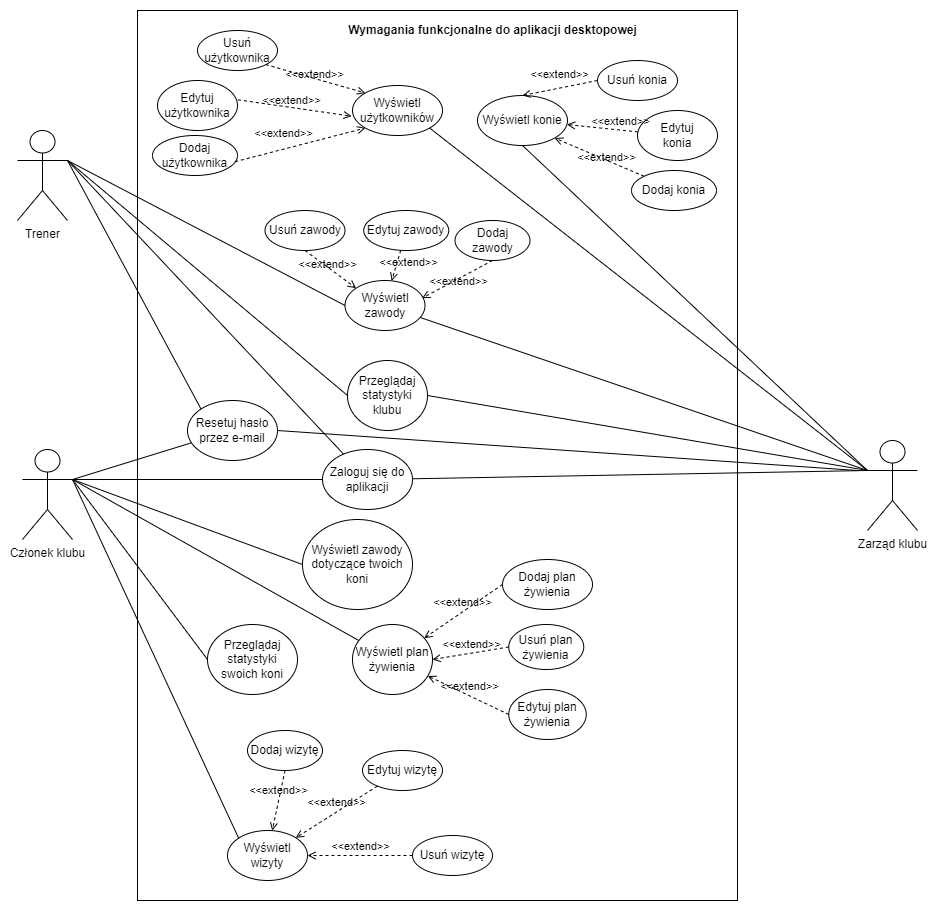
\includegraphics[scale=0.5]{UseCaseDesktop}
	\caption{Diagram Use Case dla aplikacji desktopowej}
	\textit{Źródło: Opracowanie własne}
	\label{UseCaseDesktop}
\end{figure}

\begin{figure}[H]
	\centering
	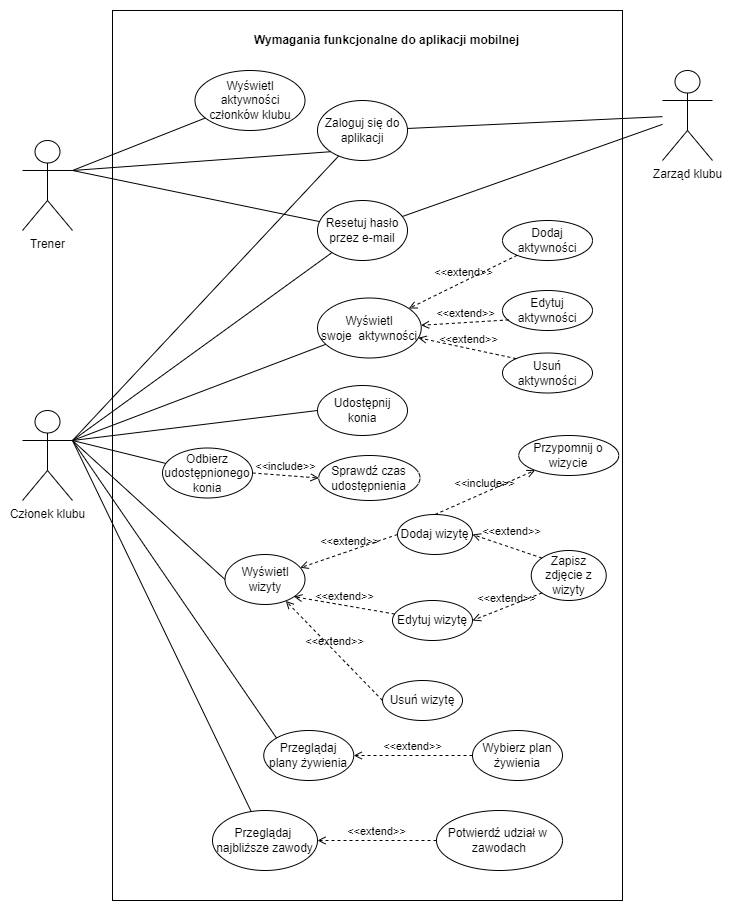
\includegraphics[scale=0.6]{UseCaseMobile}
	\caption{Diagram Use Case dla aplikacji mobilnej}
	\textit{Źródło: Opracowanie własne}
	\label{UseCaseMobile}
\end{figure}
\newpage
\section{Wymagania niefunkcjonalne}
W tym rozdziale przedstawione zostana wymagania niefunkcjonalne projektowanego systemu. W osobnych tabelach przedstawione zostaną wymagania dla aplikacji mobilnej (tabela \ref{WymaganiaNFmobilne}) oraz desktopowej (tabela \ref{WymaganiaNFdesktop}). 
Przedstawione wymagania zostały opracowane zgodnie ze standardem ISO 9126. Określone zostały atrybuty, takie jak: niezawodność (Reliability), obsługiwalność(Usability), wydajność(Efficiency), łatwość konserwacji (Maintainability) i przenośność(Portability). Na początek przedstawione zostały wymagania dla aplikacji desktopowej.
	\begin{table}[H]
	\caption{Wymagania niefunkcjonalne aplikacji desktopowej }
	\textit{Źródło: Opracowanie własne}
	\label{WymaganiaNFdesktop}
	\centering
	\begin{tabular}{|c|p{6cm}|p{8cm}|}
		\hline
		Nr & Nazwa wymagania & Opis wymagania\\
		\hline
		1& Interfejsy programowe& System operacyjny Microsoft Windows 7 lub nowszy. Baza danych zainstalowana na platformie Microsoft SQL Server 2019 lub nowszej oraz dostępna dla aplikacji zgodnie z zasadami określonymi w dokumentacji serwera.\\		
		\hline
		2& Interfejsy sprzętowe& Komputer osobisty lub laptop, obsługujący system Windows 7 lub nowszy. Minimum 4 GB pamięci RAM i xGB wolnej przestrzeni na dysku, procesor 1GHz lub szybszy, 32 bitowy (x86) lub 64 bitowy (x64).\\	
		\hline	
		3& Obsługiwaloność (Usability)& Aplikacja powinna mieć prosty i intuicyjny interfejs użytkownika. Interfejs powinien być dostosowany do pracy na monitorach o małej rozdzielczości i laptopach.\\		
		\hline
		4& Niezawodność (Reliability)& Aplikacja powinna walidować wszystkie pola, do których wprowadzane są dane. W przypadku błędnych danych powinny wyświetlać się komunikaty informujące o nieprawidłowościach w klarowny sposób.\\	
						\hline
	\end{tabular}
\end{table}
\begin{table}[H]
	\begin{tabular}{|c|p{6cm}|p{8cm}|}
		\hline
		5& Język i narzędzia programowania& Aplikacja została napisana w C\# na silniku graficznym Windows Presentation Foundation przy użyciu środowiska  Microsoft Visual Studio Community 2022.
		Baza danych została napisana w języku SQL, przy pomocy środowiska Microsoft SQL Server Management Studio 18 i zainstalowana na serwerze bazy danych Microsoft SQL Server 2019\\	

					\hline
		6& Aspekty prawne& W bazie danych przechowywane będą dane członków klubu, zarządu, specjalistów oraz których korzystają. Poza danymi osobowymi tych osób przechowywane będą także dane o koniach, ich aktywnościach oraz stanie zdrowia. Aplikacja nie będzie przekazywać danych ososobowych poszczególnych członków innym użytkownikom.Dane specjalistów będą rozpowszechniane między użytkownikami, dlatego przed wpisaniem do bazy będą musieli wyrazić na to pisemną zgodę.\\	
				\hline
		7& Wydajność (Efficiency)& Używanie aplikacji na sprzęcie o minimalnych wymaganiach powinno przebiegać w sposób płynny, to znaczy wyświetlanie, dodawanie, edytowanie, usuwanie, kategoryzowanie i filtrowanie danych powinno nie zajmować dłużej niż kilka sekund.\\	
		\hline
		8& Łatwość konserwacji (Maintainability)& Działanie aplikacji będzie kontrolowane przy pomocy dziennika debugowania. Kolejne wersje systemu (kopie zapasowe) będą zapisywane za pomocą systemu kontroli wersji GIT.\\	
								\hline
	\end{tabular}
\end{table}
\begin{table}[H]
	\begin{tabular}{|c|p{6cm}|p{8cm}|}
		\hline
		9& Przenośność (Portability)& Aplikacja udostępniana będzie w pliku wykonywalnym .exe. Baza danych musi zostać zainstalowana i skonfigurowana na serwerze w danym klubie jeździeckim. Po zainstalowaniu aplikacja i baza danych powinny zostać skonfigurowane ze sobą.\\
		\hline
	\end{tabular}
\end{table}
Następnie w tabeli \ref{WymaganiaNFmobilne} przedstawiono wymagania dla aplikacji mobilnej. Zostały one podzielone na takie same sekcje jak wymagania aplikacji desktopowej. Mimo to wymagania przedstawione zostały w oddzielnej tabeli, ponieważ dotyczą one aplikacji na całkowicie inny system.
\begin{table}[H]
	\caption{Wymagania niefunkcjonalne aplikacji mobilnej }
	\textit{Źródło: Opracowanie własne}
	\label{WymaganiaNFmobilne}
	\centering
	\begin{tabular}{|c|p{6cm}|p{8cm}|}
		\hline
		Nr & Nazwa wymagania & Opis wymagania\\
		\hline
		1& Interfejsy programowe& Android ?? lub nowszy \\		
		\hline
		2& Interfejsy sprzętowe& Telefon lub tablet z systemem operacyjnym Android ?? lub nowszym \\	
		\hline	
		3& Obsługiwaloność (Usability)& 
		Aplikacja powinna dobrze skalować się na różnej wielkości ekrany. Na telefonie najważniejsze przyciski powinny znajdować się "w zasięgu kciuka". Ikony i przyciski powinny być widoczne i możliwe do kliknięcia nawet małych ekranach (minimalny ekran ??), w aplikacji dostępny jest jedynie tryb jasny.\\		
		\hline
		4& Niezawodność (Reliability)&Aplikacja powinna walidować wszystkie pola, do których wprowadzane są dane. W przypadku błędnych danych powinny wyświetlać się komunikaty informujące o nieprawidłowościach w klarowny sposób. \\	
		\hline
						\end{tabular}
	\end{table}

\begin{table}[H]
\begin{tabular}{|c|p{6cm}|p{8cm}|}
\hline
		5& Język i narzędzia programowania& Aplikacja została napisana na platformie Xamarin przy użyciu środowiska  Microsoft Visual Studio Community 2022. Używa tej samej bazy co aplikacja desktopowa. \\	
		\hline
		6& Aspekty prawne& Aspekty prawne aplikacji mobilnej i desktopowej pokrywają się, ponieważ korzystają one z tych samych danych.\\	
		\hline
		7& Wydajność (Efficiency)&
		Używanie aplikacji na sprzęcie o minimalnych wymaganiach powinno przebiegać w sposób płynny, to znaczy wyświetlanie, dodawanie, edytowanie, usuwanie danych powinno nie zajmować dłużej niż kilka sekund. \\	
		\hline	
		8& Łatwość konserwacji (Maintainability)&
		Konserwacja aplikacji mobilnej będzie przebiegać analogicznie do desktopowej. \\	
		\hline
		9& Przenośność (Portability)&Aplikacja udostępniana w postaci pakietu instalacyjnego .apk oraz powinna spełniać wszystkie wymagania do umieszczenia jej w sklepie Google Play. \\
		\hline
	\end{tabular}
\end{table}

\newpage
\chapter{Baza danych}
W tym rozdziale przedstawimy model konceptualny, logiczny oraz fizyczny bazy danych. Rozdział ten został opracowany na podstawie \cite{bazydanych}.
\section{Model konceptualny}
Proces tworzenia bazy danych zaczynamy od modelu konceptualnego. W pierwszej fazie tworzenia go ważne jest określenie słownika pojęć, które będą następnie używane w projekcie bazy danych.
\subsubsection{Słownik pojęć}
\begin{itemize}
	\item \textbf{Użytkownik} - wszyscy członkowie klubu, trenerzy oraz zarząd klubu.
	\item \textbf{Koń} - koń należący do któregoś z członków klubu jeździeckiego, lub dzierżawiony przez niego.
	\item \textbf{Atywności} - są to czynności wykonywane przez konia w ciągu dnia, należą do nich jazdy, skoki przez przeszkody, kross, ujeżdżenie, lonża, wyjazd w teren, karuzela, padok, wyjazd na zawody, spacer, skoki luzem, padok.
	\item \textbf{Wizyty} - to wizyty wszelkich lekarzy, jak także wizyty kowali.
	\item \textbf{Udostępnianie konia} - jest to przekazanie możliwości wprowadzania danych o danym koniu przez jego właściciela innemu członkowi klubu.
	
\end{itemize}
\newpage
Po określeniu definicji poszczególnych pojęć używanych w projekcie możemy określić reguły funkcjonowania naszej aplikacja.
\subsubsection{Reguły funkcjonowania}
Reguły funkcjonowania określają zasady, procedury i wytyczne jakie musi spełniać projektowana aplikacja. 
\begin{enumerate}[start=1,label={\bfseries REG\textbackslash 00\arabic*}]
	\item Konta użytkowników tworzy jedynie użytkownik "administrator".
	\item Każdy użytkownik ma określony swój typ.
	\item Każdy użytkownik może zmienić swoje hasło.
	\item O każdym użytkowniku, jak także o lekarzu i kowalu zbieramy podstawowe dane personalne.
	\item Tylko użytkownik "administrator" dodaje konie do kont użytkowników.
	\item Każdy koń ma przypisaną płeć.
	\item Każdy koń ma przypisany status.
	\item Jeden użytkownik może posiadać wiele koni.
	\item Aktywności konia może dodać jego właściciel lub osoba której właściciel udostępni konia.
\end{enumerate}
\begin{enumerate}[start=10,label={\bfseries REG\textbackslash 0\arabic*}]
	\item Koń może mieć wiele aktywności każdego dnia.
	\item Wizyty konia może dodawać tylko jego właściciel.
	\item Na wizycie jest jeden koń i jedne lekarz/kowal.
	\item Każdy lekarz ma określoną specjalizacje.
	\item Plan żywienia konia może ustalać tylko właściciel. 
	\item Koń może posiadać wiele planów żywienia, ale aktualnie może jeść tylko jeden.
	\item Plan żywienia zawiera wiele żywień.
	\item Żywienie dotyczy konkretnego typu jedzenia, podawanego o konkretnej porze (rano, południe, wieczór), który swoją jednostkę miary.
	\item Użytkownicy, którym ktoś udostępnił konia mogą tylko wyświetlić plan żywienia.
	\item Statystyki mają być tworzone na podstawie aktywności.
	\item Użytkownik "członek klubu" może przeglądać statystyki tylko swoich koni.
	\item Użytkownik "trener" lub "administrator" może przeglądać statystyki wszystkich koni.
	\item Użytkownik "trener" lub "administrator" może dodawać wyjazd na zawody dla całego klubu i zapraszać poszczególnych użytkowników.
	\item Użytkownik "członek klubu" może dodawać swoje wyjazdy na zawody.
\end{enumerate}
\subsubsection{Ograniczenia dziedzinowe}
Ograniczenia dziedzinowe to ograniczenia, które nakładane są na atrybuty w powyższych kategoriach. Wynikają one z analizy wycinka rzeczywistości i należy je uwzględnić podczas projektowania bazy danych oraz implementacji systemu.
\begin{enumerate}[start=1,label={\bfseries OGR\textbackslash 00\arabic*}]
	\item Paszport konia składa się ze znaków i cyfr postaci xxx-aaa-bb-ccccc-dd, gdzie
	\begin{itemize} 
		\item xxx - określa kraj pochodzenia konia,  
		\item aaa - oznacza kod hodowli konia, 
		\item bb- oznacza rok urodzenia konia, 
		\item ccccc - to numer paszportu konia, 
		\item dd - to numer identyfikacyjny konia w ramach hodowli.
		\end{itemize}
	\item Data wizyty konia jest wcześniejsza niż data jego urodzenia.
\end{enumerate}
\newpage
%\renewcommand{\arraystretch}{1.2}
\subsubsection{Encje}
Po określeniu kategorii, reguł funkcjonowania, ograniczeń dziedzinowych i transakcji należy przystąpić do tworzenia encji i relacji między nimi.
\\

\begin{enumerate}[start=1,label={\bfseries ENC\textbackslash0\arabic*}]
%___________________________________________________________________________________________________________
	\item \textbf{ACTIVITY} \\
	\textit{Semantyka encji} - Encja zawierająca aktywności, które koń wykonuje w ciągu dnia. Każda aktywność oprócz typu, zawiera opis, czas trwania oraz ocenę satysfakcji i intensywności jej wykonania.
	\\
	Opis atrybutów encji znajduje się w tabeli \ref{ActivityAtribute}.
	
	\begin{table}[H]
		\caption{Wykaz atrybutów encji typu Activity }
		\textit{Źródło: Opracowanie własne}
		\label{ActivityAtribute}
		\centering
		\begin{tabular}{|l|l|l|c|}
			\hline
			Nazwa atrybutu & Opis atrybutu & Typ & OBL(+) \\
			& & &  OPC(-) \\
			\hline
			\textit{activityID} & Numer identyfikujący aktywności & Liczba naturalna & + \\
			\hline
			\textit{date} & Data wykonania aktywności & Data & + \\
			\hline
			\textit{description} & Opis aktywności & Typ znakowy & - \\
			\hline
			time &  Czas trwania aktywności & Czas & - \\
			\hline
			\textit{intensivity} & Intensywność wykonanej aktywności & Liczba naturalna & + \\
			\hline
			\textit{satisfaction} & Satysfakcja wykonanej aktywności & Liczba naturalna & + \\
			\hline
			\textit{activityType} &  Typ wykonanej aktywności & Liczba naturalna & + \\
			\hline
		\end{tabular}
	\end{table}
	Klucze kandydujące: activityID \\
	Klucz główny: activityID \\
	Charakter encji: encja słaba \\
%___________________________________________________________________________________________________________
	\item \textbf{COMPETITION}\\
	\textit{Semantyka encji} - encja zawierająca dane o zawodach jeździeckich. 
	\\
	Opis atrybutów znajduje się w tabeli \ref{competitionAtribute}.
	
	\begin{table}[H]
	    \caption{Wykaz atrybutów encji typu Competition}
	    \textit{Źródło: Opracowanie własne}
	    \label{competitionAtribute}
		\centering
		\begin{tabular}{|l|l|l|c|}
			\hline
			Nazwa atrybutu & Opis atrybutu & Typ & OBL(+) \\
			& & &  OPC(-) \\
			\hline
			\textit{competitionID} & Numer identyfikujący zawody. & Liczba naturalna & + \\
			\hline
			\textit{spot} & Miejsce, w którym odbywają się zawody. & Max. znaków 200 & - \\			\hline
			\textit{date} & Data zawodów. & Data & + \\
			\hline
			\textit{description} & Opis zawodów. & Typ znakowy & - \\
			\hline
			\textit{rank} & Ranga zawodów. &  Max. znaków 50 & - \\
			\hline
		\end{tabular}
	\end{table}
	Klucze kandydujące: competitionID \\
	Klucz główny: competitionID \\
	Charakter encji: encja silna 
%___________________________________________________________________________________________________________
	\item \textbf{NOTIFICATION}\\
	\textit{Semantyka encji} - Encja zawierająca powiadomienia utworzone przez użytkowników.
\\
Opis atrybutów encji znajduje się w tabeli \ref{NotificationAtribute}.
	\begin{table}[H]
		\caption{Wykaz atrybutów encji typu Notification }
		\textit{Źródło: Opracowanie własne}
		\label{NotificationAtribute}
		\centering
		\begin{tabular}{|l|l|l|c|}
			\hline
			Nazwa atrybutu & Opis atrybutu & Typ & OBL(+) \\
			& & &  OPC(-) \\
			\hline
			\textit{notificationID} & Numer identyfikujący powiadomienie& Liczba naturalna & + \\
			\hline
			\textit{title} &  Tytuł powiadomienia & Max. znaków 30 & + \\
			\hline
			\textit{description} & Opis powiadomienia & Typ znakowy & - \\
			\hline
			\textit{sendDate} &  Data wysłania & Data & + \\
			\hline
			\textit{createdDate} &  Data stworzenia & Data & + \\
			\hline			
			\textit{turnOn} & Określenie, czy powiadomienie jest włączone & Prawda/Fałsz & + \\
			\hline
		\end{tabular}
	\end{table}
	Klucze kandydujące: notificationID \\
	Klucz główny: notificationID \\
	Charakter encji: encja słaba \\
	
%___________________________________________________________________________________________________________
	\item \textbf{PROFESSIONAL}\\
	\textit{Semantyka encji} - encja opisująca specjalistów przyjeżdżający do konia takich jak lekarze (np. gastrolog, kardiolog, lekarz ogólny), fizjoterapeuci, kowale itp.
	\\
Opis atrybutów encji znajduje się w tabeli \ref{ProfessionalsAtribute}.

	\begin{table}[H]		
		\caption{Wykaz atrybutów encji typu PROFESSIONAL }
		\textit{Źródło: Opracowanie własne}
		\label{ProfessionalsAtribute}
		\centering
		\begin{tabular}{|l|l|l|c|}
			\hline
			Nazwa atrybutu & Opis atrybutu & Typ & OBL(+) \\
			& & &  OPC(-) \\
			\hline
			\textit{professionalsID} & Numer identyfikujący specjalistę & Liczba naturalna & + \\
			\hline			
			\textit{degree} & Stopień naukowy doktora & Liczba naturalna & - \\
			\hline
		\end{tabular}

	\end{table}
	Klucze kandydujące: professionalsID \\
	Klucz główny: professionalsID \\
	Charakter encji: encja słaba 
%__________________________________________________________________________________________________________	
	\item \textbf{SPECIALISATION}\\
	\textit{Semantyka encji} - encja słownikowa zawiera nazwy specjalizacji specjalistów.
	\\
	Opis atrybutów encji znajduje się w tabeli \ref{SpecialisationAtribute}.
	
	\begin{table}[H]
		\caption{Wykaz atrybutów encji typu Specialization}
		\textit{Źródło: Opracowanie własne}
		\label{SpecialisationAtribute}
		\centering
		\begin{tabular}{|l|l|l|c|}
			\hline
			Nazwa atrybutu & Opis atrybutu & Typ & OBL(+) \\
			& & &  OPC(-) \\
			\hline
			\textit{specialisationID} & Numer identyfikujący specjalizacje & Liczba naturalna & + \\
			\hline
			\textit{name} & Nazwa specjalizacji & Max. znaków 85 & + \\
			\hline
		\end{tabular}
	\end{table}
	Klucze kandydujące: specializationID \\
	Klucz główny: specializationID \\
	Charakter encji: encja silna \\
	\newpage
	\item \textbf{DIET}
	
		\textit{Semantyka encji} - Encja zawierająca informacje o aktywnej diecie konia. 
		\\
	Opis atrybutów encji znajduje się w tabeli \ref{DietAtribute}.
	
	\begin{table}[H]
		\caption{Wykaz atrybutów encji typu Diet }
		\textit{Źródło: Opracowanie własne}
		\label{DietAtribute}
		\centering
		\begin{tabular}{|l|l|l|c|}
			\hline
			Nazwa atrybutu & Opis atrybutu & Typ & OBL(+) \\
			& & &  OPC(-) \\
			\hline
			\textit{dietID} & Numer identyfikujący dietę & Liczba naturalna & + \\
			\hline
			\textit{isActive} & Określenie czy plan jest w użyciu & Prawda/Fałsz & + \\
			\hline
		\end{tabular}

	\end{table}
	Klucze kandydujące: dietID \\
	Klucz główny: dietID \\
	Charakter encji: encja słaba
	
	\item \textbf{PORTION}
	
	\textit{Semantyka encji} - Encja zawierająca informacje o porcji jedzenia.
	\\
	Opis atrybutów encji znajduje się w tabeli \ref{DietAtribute}.
	
	\begin{table}[H]
		\caption{Wykaz atrybutów encji typu Portion}
		\textit{Źródło: Opracowanie własne}
		\label{PortionAtribute}
		\centering
		\begin{tabular}{|l|l|l|c|}
			\hline
			Nazwa atrybutu & Opis atrybutu & Typ & OBL(+) \\
			& & &  OPC(-) \\
			\hline
			\textit{portionID} & Numer identyfikujący jedzenie & Liczba naturalna & + \\
			\hline
			\textit{amount} &  Ilość jedzenia w porcji & Liczba zmiennoprzecinkowa & + \\
			\hline
		\end{tabular}

	\end{table}
	Klucze kandydujące: portionID \\
	Klucz główny: portionID \\
	Charakter encji: encja słaba \\
	\newpage
%___________________________________________________________________________________________________________
	\item \textbf{FORAGE}
	
	\textit{Semantyka encji} - Encja zawierająca informacje o paszy dla koni.
	\\
	Opis atrybutów encji znajduje się w tabeli \ref{ForageAtribute}.
	
	\begin{table}[H]
		\caption{Wykaz atrybutów encji typu Forage }
		\textit{Źródło: Opracowanie własne}
		\label{ForageAtribute}
		\centering
		\begin{tabular}{|l|l|l|c|}
			\hline
			Nazwa atrybutu & Opis atrybutu & Typ & OBL(+) \\
			& & &  OPC(-) \\
			\hline
			\textit{forageID} & Numer identyfikujący paszy & Liczba naturalna & + \\
			\hline
			\textit{name} &  Nazwa paszy & Max. znaków 92 & + \\
			\hline
			\textit{producent} & Producent paszy & max. znaków 57 & - \\
			\hline
			\textit{capacity} & Ilość paszy w jednym worku & Liczba naturalna & - \\
			\hline
		\end{tabular}
	\end{table}
	Klucze kandydujące: forageID \\
	Klucz główny: forageID \\
	Charakter encji: encja słaba
	\item \textbf{HORSE}
	
	\textit{Semantyka encji} - Encja zawierająca wszystkie informacje o koniach.
	\\
	Opis atrybutów encji znajduje się w tabeli \ref{HorseAtribute}.
	
	\begin{table}[H]
		\caption{Wykaz atrybutów encji typu Horse }
		\textit{Źródło: Opracowanie własne}
		\label{HorseAtribute}
		\centering
		\begin{tabular}{|l|l|l|c|}
			\hline
			Nazwa atrybutu & Opis atrybutu & Typ & OBL(+) \\
			& & &  OPC(-) \\
			\hline
			\textit{horseID} & Numer identyfikujący konia & Liczba naturalna & + \\
			\hline
			\textit{name} &  Imie konia & max. znaków 60 & + \\
			\hline
			\textit{mother} &  Imie klaczy & max. znaków 60 & - \\
			\hline
			\textit{father} &  Imie ogiera & Max. znaków 60 & - \\
			\hline
			\textit{birthday} & Data urodzenia konia & Date & - \\
			\hline
			\textit{race} &  Rasa konia & Max. znaków 50 & - \\
			\hline
			\textit{breeder} &  Hodowca koni & Max. znaków 60 & - \\
			\hline
			\textit{passport} & Paszport konia & Max. znaków 20 & - \\
			\hline
			\textit{photo} & Zdjęcie konia & Typ znakowy & - \\
			\hline
		\end{tabular}
	\end{table}
	Klucze kandydujące: horseID \\
	Klucz główny: horseID \\
	Charakter encji: encja słaba
\end{enumerate}

\begin{enumerate}[start=10,label={\bfseries ENC$\backslash$\arabic*}]
	\item \textbf{HORSEGENDER} \\
	\textit{Semantyka encji} - Encja słownikowa zawierająca płeć koni.
	\\
	Opis atrybutów encji znajduje się w tabeli \ref{HorseGenderAtribute}.
	
	\begin{table}[H]
		\caption{Wykaz atrybutów encji typu HorseGender }
		\textit{Źródło: Opracowanie własne}
		\label{HorseGenderAtribute}
		\centering
		\begin{tabular}{|l|l|l|c|}
			\hline
			Nazwa atrybutu & Opis atrybutu & Typ & OBL(+) \\
			& & &  OPC(-) \\
			\hline
			\textit{genderID} & Numer identyfikujący płeć konia & Liczba naturalna & + \\
			\hline
			\textit{gender} &  Nazwa płci konia & Max. znaków 10 & + \\
			\hline
		\end{tabular}
	\end{table}
	Klucze kandydujące: genderID \\
	Klucz główny: genderID \\
	Charakter encji: encja silna
	\item \textbf{STATUS}
	
	\textit{Semantyka encji} - Encja słownikowa zawierająca statusy koni.
		\\ 
	Opis atrybutów encji znajduje się w tabeli \ref{StatusAtribute}.
	
	\begin{table}[H]
		\caption{Wykaz atrybutów encji typu Status}
		\textit{Źródło: Opracowanie własne}
		\label{StatusAtribute}
		\centering
		\begin{tabular}{|l|l|l|c|}
			\hline
			Nazwa atrybutu & Opis atrybutu & Typ & OBL(+) \\
			& & &  OPC(-) \\
			\hline
			\textit{statusID} & Numer identyfikujący status konia & Liczba naturalna & + \\
			\hline
			\textit{name} &  Nazwa statusu konia & Max. znaków 20 & + \\
			\hline
		\end{tabular}
	\end{table}
	Klucze kandydujące: statusID \\
	Klucz główny: statusID \\
	Charakter encji: encja silna
	\item \textbf{MEALNAME} \\
	\textit{Semantyka encji} - Encja słownikowa zawierająca nazwy posiłków.
		\\ 
Opis atrybutów encji znajduje się w tabeli \ref{MealNameAtribute}.
	
	\begin{table}[H]
		\caption{Wykaz atrybutów encji typu MealName }
		\textit{Źródło: Opracowanie własne}
		\label{MealNameAtribute}
		\centering
		\begin{tabular}{|l|l|l|c|}
			\hline
			Nazwa atrybutu & Opis atrybutu & Typ & OBL(+) \\
			& & &  OPC(-) \\
			\hline
			\textit{mealNameID} & Numer identyfikujący posiłek & Liczba naturalna & + \\
			\hline
			\textit{mealName} & Nazwa posiłku & Max. znaków 20 & + \\
			\hline
		\end{tabular}
	\end{table}
	Klucze kandydujące: mealNameID \\
	Klucz główny: mealNameID \\
	Charakter encji: encja słaba \\
\newpage
\item \textbf{NUTRITIONPLAN}
\\ \\
\textit{Semantyka encji} - Encja zawierająca informacje o planie żywienia koni.
		\\
Opis atrybutów encji znajduje się w tabeli \ref{NutritionPlanAtribute}.

\begin{table}[H]
	\caption{Wykaz atrybutów encji typu NutrtionPlan }
	\textit{Źródło: Opracowanie własne}
	\label{NutritionPlanAtribute}
	\centering
	\begin{tabular}{|l|l|l|c|}
		\hline
		Nazwa atrybutu & Opis atrybutu & Typ & OBL(+) \\
		& & &  OPC(-) \\
		\hline
		\textit{nutritionPlanID} & Numer identyfikujący plan żywienia & Liczba naturalna & + \\
		\hline
		\textit{title} &  Tytuł planu żywienia & Max. znaków 50 & + \\
		\hline
		\textit{desctription} &  Ilość jedzenia w porcji & Typ znakowy & - \\
		\hline
		\textit{icon} &  Ikona dołączona do planu żywienia & Liczba naturalna & + \\
		\hline		
		\textit{color} &  Color dołączona do planu żywienia & Max. 7 znaków & + \\
		\hline
	\end{tabular}
\end{table}
Klucze kandydujące: nutritionPlanID \\
Klucz główny: nutritionPlanID \\
Charakter encji: encja silna\\
	\item \textbf{PEOPLEDETAILS}\\ \\
	\textit{Semantyka encji} - encja zawiera szczegółowe dane użytkowników (członków klubu, trenerów i zarządu klubu) jak i lekarzy oraz kowali.
			\\ 
	Opis atrybutów encji znajduje się w tabeli \ref{PeopleDetailsAtribute}.
	
	\begin{table}[H]
    	\caption{Wykaz atrybutów encji typu PeopleDetails }
    	\textit{Źródło: Opracowanie własne}
    	\label{PeopleDetailsAtribute}
		\centering
		\begin{tabular}{|l|l|l|c|}
			\hline
			Nazwa atrybutu & Opis atrybutu & Typ & OBL(+) \\
			 & & &  OPC(-) \\
			\hline
			\textit{detailsID} & Numer identyfikujący dane użytkowników & Liczba naturalna & + \\
			\hline
			\textit{name} & Imie & Max. znaków 40 & - \\
			\hline
			\textit{surname} & Nazwisko & Max. znaków 40 & + \\
			\hline
			\textit{phonNumber} & Numer telefonu & Max. znaków 20 & - \\
			\hline
			\textit{email} & Adres e-mailowy & Max. znaków 320 & - \\
			\hline
			\textit{city} & Miasto zamieszkania & Max. znaków 200 & - \\
			\hline
			\textit{street} & Ulica zamieszkania & Max. znaków 90 & - \\
			\hline
			\textit{number} & Numer domu zamieszkania & Max. znaków 10 & - \\
			\hline
		\end{tabular}
	\end{table}
Klucze kandydujące: detailsID \\
Klucz główny: detailsID \\
Charakter encji: encja silna
\item \textbf{PARTICIPATION}\\ 
\textit{Semantyka encji} - encja zawierająca dane o uczestnictwie konia w zawodach.
			\\ 
Opis atrybutów encji znajduje się w tabeli \ref{ParticipationAtribute}.

\begin{table}[H]
	\caption{Wykaz atrybutów encji typu Participation }
	\textit{Źródło: Opracowanie własne}
	\label{ParticipationAtribute}
	\centering
	\begin{tabular}{|l|l|l|c|}
		\hline
		Nazwa atrybutu & Opis atrybutu & Typ & OBL(+) \\
		& & &  OPC(-) \\
		\hline
		\textit{participationID} & Numer identyfikujący udział w zawodach & Liczba naturalna & + \\
		\hline
		\textit{result} & Wynik zawodów & Typ znakowy & + \\
		\hline
		\textit{place} & Zajęte miejsce &  Liczba naturalna & + \\
		\hline
	\end{tabular}
\end{table}
Klucze kandydujące: participationID \\
Klucz główny: participationID \\
Charakter encji: encja słaba \\

\item \textbf{SHARED}

\textit{Semantyka encji} - Encja zawierająca wpisy o udostępnianiu koni.
			\\ \\
Opis atrybutów encji znajduje się w tabeli \ref{SharedAtribute}.

\begin{table}[H]
	\caption{Wykaz atrybutów encji typu Shared }
	\textit{Źródło: Opracowanie własne}
	\label{SharedAtribute}
	\centering
	\begin{tabular}{|l|l|l|c|}
		\hline
		Nazwa atrybutu & Opis atrybutu & Typ & OBL(+) \\
		& & &  OPC(-) \\
		\hline
		\textit{sharedID} & Numer identyfikujący status konia & Liczba naturalna & + \\
		\hline
		\textit{code} &  Kod z kodu QR & Max. znaków 50 & + \\
		\hline
		\textit{endDate} &  Data kończąca udostępnienie & Data & + \\
		\hline
		\textit{startDate} &  Data udostępnienia & Data & + \\
		\hline
	\end{tabular}
\end{table}
Klucze kandydujące: sharedID \\
Klucz główny: sharedID \\
Charakter encji: encja słaba \\


\item \textbf{UNITOFMEASURE}

\textit{Semantyka encji} - Encja słownikowa zawierająca nazwy jednostek miary.
			\\ \\
Opis atrybutów encji znajduje się w tabeli \ref{UnitOfMeasure}.

\begin{table}[H]
	\caption{Wykaz atrybutów encji typu UnitOfMeasure }
	\textit{Źródło: Opracowanie własne}
	\label{UnitOfMeasure}
	\centering
	\begin{tabular}{|l|l|l|c|}
		\hline
		Nazwa atrybutu & Opis atrybutu & Typ & OBL(+) \\
		& & &  OPC(-) \\
		\hline
		\textit{unitID} & Numer identyfikujący jednostkę miary & Liczba naturalna & + \\
		\hline
		\textit{unitName} & Nazwa jednostek miary & Max. znaków 30 & + \\
		\hline
	\end{tabular}
\end{table}
Klucze kandydujące: unitID \\
Klucz główny: unitID \\
Charakter encji: encja silna \\

\item \textbf{UserAcount}\\ \\
\textit{Semantyka encji} - encja zawiera dane użytkownika (członków klubu, trenerów i zarządu klubu).
			\\ \\
Opis atrybutów encji znajduje się w tabeli \ref{UserAcountAtribute}.

\begin{table}[H]
	\caption{Wykaz atrybutów encji typu UserAcount }
	\textit{Źródło: Opracowanie własne}
	\label{UserAcountAtribute}
	\centering
	\begin{tabular}{|l|l|l|c|}
		\hline
		Nazwa atrybutu & Opis atrybutu & Typ & OBL(+) \\
		& & &  OPC(-) \\
		\hline
		\textit{userID} & Numer identyfikujący użytkownika & Liczba naturalna & + \\
		\hline
		\textit{login} & Login użytkownika & max. znaków 50 & + \\
		\hline
		\textit{hash} & Hash hasła użytkownika & max. znaków 50 & + \\
		\hline
		\textit{salt} & Salt hasła użytkownika & max. znaków 50 & + \\
		\hline
		\textit{createdDateTime} & Data utworzenia konta & Data & + \\
		\hline
	\end{tabular}
\end{table}
Klucze kandydujące: userID \\
Klucz główny: userID \\
Charakter encji: encja słaba \\

\item \textbf{USERTYPE} \\ \\
\textit{Semantyka encji} - encja zawiera typy użytkowników: zwykły użytkownik (standard), trener (trainer), zarząd klubu (admin).
			\\ \\
Opis atrybutów encji znajduje się w tabeli \ref{UserTypeAtribute}.

\begin{table}[H]
	\caption{Wykaz atrybutów encji typu UserType }
	\textit{Źródło: Opracowanie własne}
	\label{UserTypeAtribute}
	\centering
	\begin{tabular}{|l|l|l|c|}			
		\hline
		Nazwa atrybutu & Opis atrybutu & Typ & OBL(+) \\
		& & &  OPC(-) \\
		\hline
		\textit{userTypeID} & Numer identyfikujący typ użytkownika & Liczba naturalna & + \\
		\hline
		\textit{typeName} & Nazwa typu użytkownika & max. znaków 20 & + \\
		\hline
	\end{tabular}
\end{table}
Klucze kandydujące: userTypeID \\
Klucz główny: userTypeID \\
Charakter encji: encja silna \\

%_______________________________________________________________________________________________________________________________
\item \textbf{VISIT}\\ \\
\textit{Semantyka encji} - encja zawierająca dane o wizytach. 			
\\ \\
Opis atrybutów encji znajduje się w tabeli \ref{VisitAtribute}.

\begin{table}[H]
	\caption{Wykaz atrybutów encji typu Visit }
	\textit{Źródło: Opracowanie własne}
	\label{VisitAtribute}
	\centering
	\begin{tabular}{|l|l|l|c|}
		\hline
		Nazwa atrybutu & Opis atrybutu & Typ & OBL(+) \\
		& & &  OPC(-) \\
		\hline
		\textit{visitID} & Numer identyfikujący wizyte & Liczba naturalna & + \\
		\hline
		\textit{cost} & Cena wizyty & Liczba rzeczywista dodatnia & - \\
		\hline
		\textit{summary} & Opis podsumowujący wizytę & Typ znakowy & - \\
		\hline
		\textit{artefactImage} & Zdjęcie z wizyty & Typ znakowy & - \\
		\hline
		\textit{visitDate} & Data wizyty & Data & + \\
		\hline
	\end{tabular}
\end{table}
Klucze kandydujące: visitID \\
Klucz główny: visitID \\
Charakter encji: encja słaba \\

\item \textbf{MEAL} \\
\textit{Semantyka encji} - Encja słownikowa zawierająca posiłki.
\\ \\
Opis atrybutów encji znajduje się w tabeli \ref{MealAtribute}.

\begin{table}[H]
	\caption{Wykaz atrybutów encji typu Meal}
	\textit{Źródło: Opracowanie własne}
	\label{MealAtribute}
	\centering
	\begin{tabular}{|l|l|l|c|}
		\hline
		Nazwa atrybutu & Opis atrybutu & Typ & OBL(+) \\
		& & &  OPC(-) \\
		\hline
		\textit{mealID} & Numer identyfikujący posiłek & Liczba naturalna & + \\
		\hline
		\textit{hour} & Godzina podawania posiłku & Max. znaków 10 & - \\
		\hline
	\end{tabular}
\end{table}
Klucze kandydujące: mealID \\
Klucz główny: mealID \\
Charakter encji: encja słaba \\

\item \textbf{CONTEST} \\
\textit{Semantyka encji} - Encja zawierająca konkursy z zawodów.
\\ \\
Opis atrybutów encji znajduje się w tabeli \ref{ContestAtribute}.

\begin{table}[H]
	\caption{Wykaz atrybutów encji typu Contest}
	\textit{Źródło: Opracowanie własne}
	\label{ContestAtribute}
	\centering
	\begin{tabular}{|l|l|l|c|}
		\hline
		Nazwa atrybutu & Opis atrybutu & Typ & OBL(+) \\
		& & &  OPC(-) \\
		\hline
		\textit{contestID} & Numer identyfikujący posiłek & Liczba naturalna & + \\
		\hline
		\textit{level} & Poziom konkursu & Max. znaków 10 & - \\
		\hline		
		\textit{name} & Nazwa konkursu & Max. znaków 50 & - \\
		\hline
	\end{tabular}
\end{table}
Klucze kandydujące: contestID \\
Klucz główny: contestID \\
Charakter encji: encja słaba \\
\end{enumerate}
\newpage
Po zaprojektowaniu encji możemy zapisać predykatowe definicje typów encji:
\begin{enumerate}[start=1,label={\bfseries ENC$\backslash$0\arabic*}]
	\item \textbf{ACTIVITY}(\textit{\underline{activityID}, date, description, time, intensivity, satisfaction, activityType})
	\item \textbf{COMPETITION} (\textit{\underline{competitionID}, spot, description, rank, date})
	\item \textbf{NOTIFICATION} (\textit{\underline{notificationID}, title, description, sendDate, createdDate, turnOn})
	\item \textbf{PROFESTIONALS} (\textit{\underline{profesionalsID}}, degree)
	\item \textbf{SPECIALISATION} (\textit{\underline{specialisationID}, name})
	\item \textbf{DIET} (\textit{\underline{dietID}, isActive})
	\item \textbf{PORTION} (\textit{\underline{portionID}, amount})
	\item \textbf{FORAGE} (\textit{\underline{forageID}, name, producent, capacity})
	\item \textbf{HORSE} (\textit{\underline{horseID}, name, mother, father, birthday, race, breeder, passport, photo})
\end{enumerate}
\begin{enumerate}[start=10,label={\bfseries ENC$\backslash$\arabic*}]
	\item \textbf{HORSEGENDER} (\textit{\underline{genderID}, gender})
	\item \textbf{STATUS} (\textit{\underline{statusID}, name})
	\item \textbf{MEALNAME} (\textit{\underline{mealNameID}, mealName})
	\item \textbf{NUTRITIONPLAN} (\underline{nutritionPlanID}, title, description, icon, color)
	\item \textbf{PEOPLEDETIALS} (\underline{detailsID}, name, surname, phone, email, city, street, number)
	\item \textbf{PARTICIPATION} (\underline{participationID}, result, place)
	\item \textbf{SHARED} (\underline{sharedID}, code, endDate, startDate)
	\item \textbf{UNITOFMEASURE} (\underline{unitID}, unitName)
	\item \textbf{USERACCOUNT} (\underline{userID}, accountLogin, hash, salt, createdDateTime)
	\item \textbf{USERTYPE} (\underline{userTypeID}, typeName)
	\item \textbf{VISIT} (\underline{careID}, cost, summary, artefactImage, visitDate)
    \item \textbf{MEAL} (\textit{\underline{mealID}, hour})    
    \item \textbf{CONTEST} (\textit{\underline{contestID}, level, name})
\end{enumerate}
\newpage
	Predykatowe definicje związków encji:

	\begin{enumerate}[start=0,label={\bfseries ZWI$\backslash$xx}]
		\item \textbf{Związek} (ENCJA1(min, max) ENCJA2(min, max))
	\end{enumerate}
	\begin{enumerate}[start=1,label={\bfseries ZWI$\backslash$0\arabic*}]
		\item \textbf{Has} (HORSE(0,N) HORSEGENDER(1,1))
		\item \textbf{Has} (HORSE(0,N) HORSESTATUS(1,1))
		\item \textbf{Take} (HORSE(1,1) PARTICIPATION(0,N))
		\item \textbf{Refers to} (PARTICIPATION(0,N) COMPETITION(1,1))
		\item \textbf{Performs} (HORSE(1,1) ACTIVITY(0,N))
		\item \textbf{Train} (ACTIVITY(1,1) USERACOUNT(0,N))		
		\item \textbf{Ride} (ACTIVITY(1,1) USERACOUNT(0,N))
		\item \textbf{Refers to} (NOTIFICATION(0,N) USERACOUNT(1,1))		
		\item \textbf{Refers to} (NOTIFICATION(0,N) Horse(1,1))	
	\end{enumerate}
	\begin{enumerate}[start=10,label={\bfseries ZWI$\backslash$\arabic*}]	
		\item \textbf{Gets} (USERACOUNT(1,1) SHARE(0,N))
		\item \textbf{Shares} (USERACCOUNT(1,1) SHARE(0,N))
		\item \textbf{IsShared} (HORSE(1,1) SHARE(0,N))
		\item \textbf{Has} (USERACCOUNT(0,N), USERTYPE(1,1))
		\item \textbf{Concern} (PEOPLEDETAILS(1,1) USERACCOUNT(0,N))
		\item \textbf{Attend} (HORSE(1,1) VISIT(0,N))
		\item \textbf{CareOn} (VISIT(0,N) PROFESSIONALS(1,1))
		\item \textbf{Has} (PROFESSIONALS(0,N) SPECIALISATION(1,1))
		\item \textbf{IsOn} (HORSE(1,1) DIET(0,N))
		\item \textbf{Contains} (DIET(0,N) NUTRITIONPLAN(1,1))
		\item \textbf{BelongsTo} (MEAL(0,N) NUTRITIONPLAN(0,1))
		\item \textbf{Has} (MEALNAME(1,1) MEAL(0,N))		
		\item \textbf{ConsistOf} (MEAL(1,1) PORTION(0,N))
		\item \textbf{Contains} (PORTION(0,N) FORAGE(1,1))
		\item \textbf{Has} (FORAGE(0,N) UNITOFMEASURE(1,1))
		\item \textbf{Has} (PORTION(0,N) UNITOFMEASURE(1,1))
		\item \textbf{Add} (NUTRITIONPLAN(0,N) USERACCOUNT(1,1))
		\item \textbf{Has} (HORSE(0,N) USERACCOUNT(1,1))
	\end{enumerate}

Model konceptualny przedstawiony został na diagramie ERD, który został przedstawiony na rysunku \ref{DiagramERD}.
\begin{figure}[H]
	\centering
		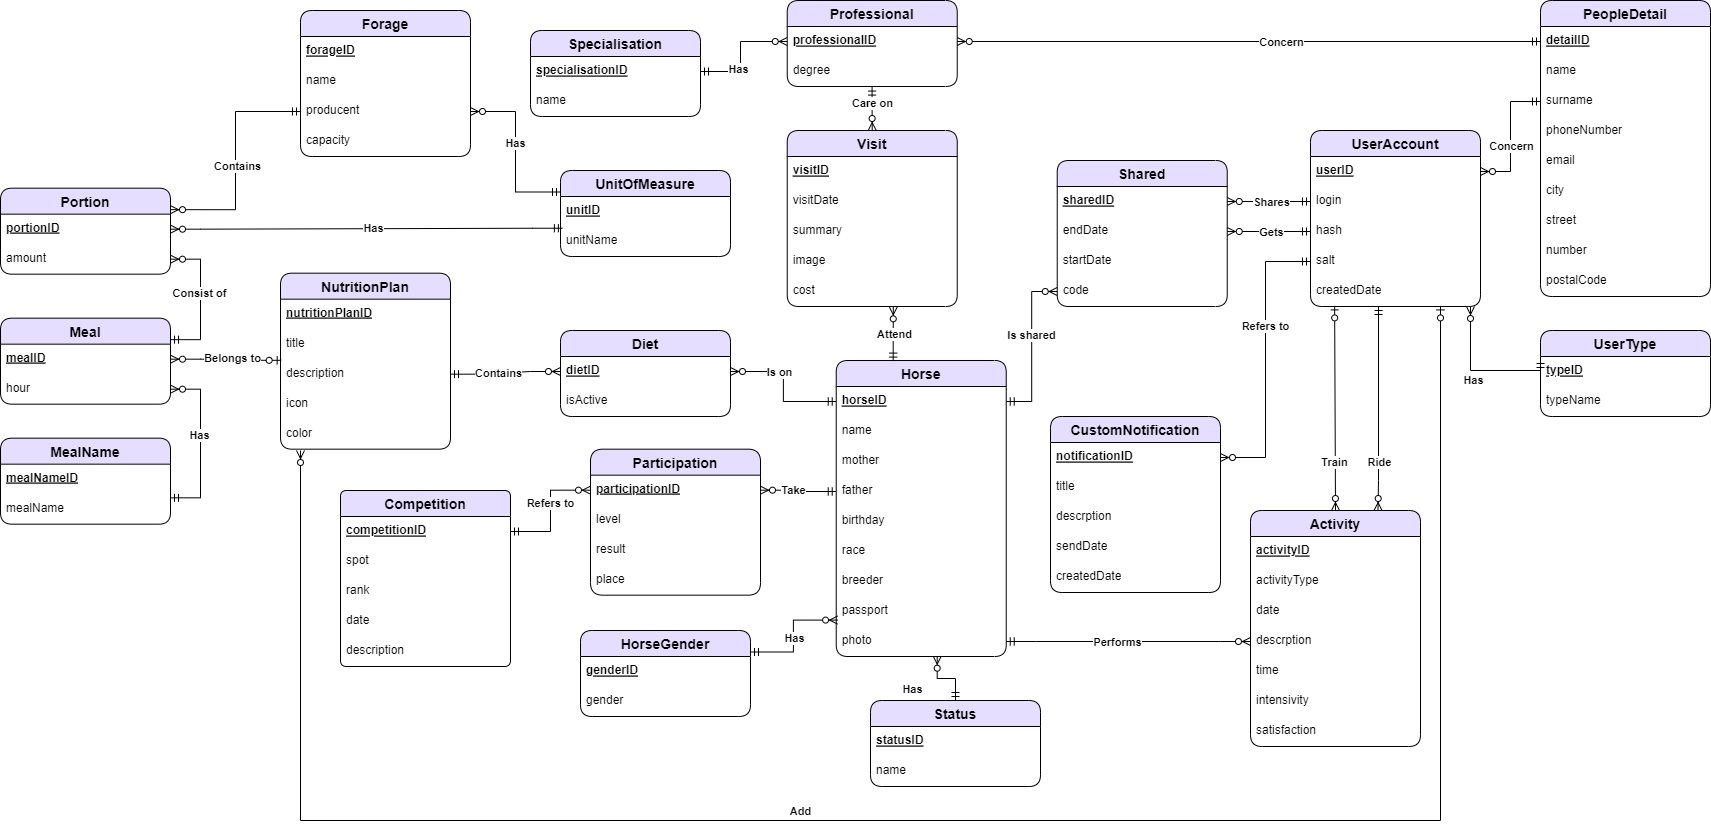
\includegraphics[scale=0.35, angle=-90]{DiagramERD}
		\caption{Diagram ERD}
		\textit{Źródło: Opracowanie własne}
		\label{DiagramERD}
\end{figure}
\section{Model logiczny}
Po stworzeniu modelu konceptualnego, należy przetransformować go do modelu logicznego. Poniżej przedstawiono tabele opisujące schematy relacji oraz znaczenia atrybutów tych relacji.
\begin{enumerate}[start=1,label={\bfseries REL\textbackslash0\arabic*}]
	\item \textbf{Activities\textbackslash ACTIVITY} \\
	Opis schematu relacji znajduje się w tabeli \ref{ActivityRelationSchema}.
	
	\begin{table}[H]
		\caption{Opis schematu relacji Activities}
		\textit{Źródło: Opracowanie własne}
		\label{ActivityRelationSchema}
		\centering
		\begin{tabular}{|c|c|c|c|c|c|c|c|c|c|}
			\hline
			\begin{sideways}Nazwa atrybutu\end{sideways}& 
			\begin{sideways}Dziedzina \end{sideways}& 
			\begin{sideways}Maska \end{sideways}& 
			\begin{sideways}OBL(+) OPC(-)\end{sideways} & 
			\begin{sideways}Wartość domyślna$\ $\end{sideways}& 
			\begin{sideways}Ograniczenia\end{sideways} &
			\begin{sideways}Unikalność \end{sideways}& 
			\begin{sideways}Klucz \end{sideways}& 
			\begin{sideways}Referencje \end{sideways}&
			\begin{sideways}Źródło danych\end{sideways}\\
			\hline
			\textit{activityID} & Integer+ & & + & & & + & PR & &SZBD\\
			\hline
			\textit{date} & Date & dd-mm-rrrr& + & & & & & &USER\\
			\hline
			\textit{description} & String & & - & & & & & &USER\\
			\hline
			\textit{time} & Integer & & + & & & & & &USER\\
			\hline
			\textit{intensivity}  & Integer+ & & + & & & & & &USER\\
			\hline
			\textit{satisfaction} & Integer+ & & + & & & & & &USER\\
			\hline
			\textit{activityType} & Integer+ & & + & & & & & &USER\\
			\hline
			\textit{userID} & Integer+ & & + & & & &FK&User&BD\\
			\hline	
			\textit{horseID} & Integer+ & & + & & & &FK&Horse&BD\\
			\hline
			\textit{trainerID} & Integer+ & & - & & & &FK&User&BD\\
			\hline		
		\end{tabular}
	\end{table}

	\begin{table}[H]
	\caption{Opis atrybutów relacji Activities}
	\textit{Źródło: Opracowanie własne}
	\label{ActivityAttributeDescription}
	\centering
	\begin{tabular}{|c|c|}
\hline
Nazwa atrybutu & Znaczenie \\
\hline
\textit{activityID} & Unikalne ID aktywności, generowane przez aplikację, klucz główny tabeli. \\
\hline
\textit{date} &  Data wykonywanej aktywności.\\
\hline
\textit{description} & Opis aktywności, dowolne polskie znaki.\\
\hline
\textit{time} & Liczba naturalna, oznaczająca czas trwania wykonywanej aktywności.\\
\hline
\textit{intensivity}  & Liczba naturalna od 0 do 5 oznaczająca poziom intensywności treningu.\\
\hline
\textit{satisfaction} & Liczba naturalna od 0 do 5 oznaczająca poziom satysfakcji z treningu.\\
\hline
\textit{activityType} &  Liczba naturalna oznaczająca typ aktywności.\\
			\hline
\textit{userID} & Indentyfikator użytkownika, który wpisuje aktywność.\\
\hline	
\textit{horseID} & Identyfikator konia, którego dotyczy aktywność.\\
\hline
\textit{trainerID} & Identyfikator użytkownika typu trener, który przeprowadzał trening.\\
\hline
	\end{tabular}
\end{table}

	\item \textbf{Competitions\textbackslash COMPETITION} \\
Opis schematu relacji znajduje się w tabeli \ref{CompetitionsRelationSchema}.
\begin{table}[h!]
	\caption{Opis schematu relacji Competitions}
	\textit{Źródło: Opracowanie własne}
	\label{CompetitionsRelationSchema}
	\centering
	\begin{tabular}{|c|c|c|c|c|c|c|c|c|c|}
		\hline
		\begin{sideways}Nazwa atrybutu\end{sideways}& 
		\begin{sideways}Dziedzina \end{sideways}& 
		\begin{sideways}Maska \end{sideways}& 
		\begin{sideways}OBL(+) OPC(-)\end{sideways} & 
		\begin{sideways}Wartość domyślna$\ $\end{sideways}& 
		\begin{sideways}Ograniczenia\end{sideways} &
		\begin{sideways}Unikalność \end{sideways}& 
		\begin{sideways}Klucz \end{sideways}& 
		\begin{sideways}Referencje \end{sideways}&
		\begin{sideways}Źródło danych\end{sideways}\\
		\hline
		\textit{competitionID} & Integer+ & & + & & & + & PR & &SZBD\\
		\hline
		\textit{spot} & String & & - & & & & & &USER\\
		\hline
		\textit{rank} & String & & - & & & & & &USER\\
		\hline
		\textit{date} & Date & & + & & & & & &USER\\
		\hline
		\textit{description}  & String & & + & & & & & &USER\\
		\hline		
	\end{tabular}
\end{table}

\begin{table}[H]
	\caption{Opis atrybutów relacji Competitions}
	\textit{Źródło: Opracowanie własne}
	\label{CompetitionsAttributeDescription}
	\centering
	\begin{tabular}{|c|c|}
		\hline
		Nazwa atrybutu & Znaczenie \\
		\hline
		\textit{competitionID} & Unikalny numer ID identyfikujący zawody, generowany przez aplikację.\\
\hline
\textit{spot} & Miejsce, w którym odbędą się zawody.\\
\hline
\textit{rank} & Ranga zawodów np. regionalne/międzynarodowe itp.\\
\hline
\textit{date} & Dzień, w którym odbędą się zawody.\\
\hline
\textit{description}  & Opis zawodów.\\
\hline	
	\end{tabular}
\end{table}
\item \textbf{Notifications\textbackslash NOTIFICATION}
\begin{table}[H]
	\caption{Opis schematu relacji Notifications}
	\textit{Źródło: Opracowanie własne}
	\label{NotificationsRelationSchema}
	\centering
	\begin{tabular}{|c|c|c|c|c|c|c|c|c|c|}
		\hline
		\begin{sideways}Nazwa atrybutu\end{sideways}& 
		\begin{sideways}Dziedzina \end{sideways}& 
		\begin{sideways}Maska \end{sideways}& 
		\begin{sideways}OBL(+) OPC(-)\end{sideways} & 
		\begin{sideways}Wartość domyślna$\ $\end{sideways}& 
		\begin{sideways}Ograniczenia\end{sideways} &
		\begin{sideways}Unikalność \end{sideways}& 
		\begin{sideways}Klucz \end{sideways}& 
		\begin{sideways}Referencje \end{sideways}&
		\begin{sideways}Źródło danych\end{sideways}\\
			\hline
	\textit{notificationID} & Integer+& & + &&&+&PR&&SZBD\\
	\hline
	\textit{title} & String& & + &&&&&&USER\\
	\hline
	\textit{description}  & String& & + &&&&&&USER\\
	\hline
	\textit{sendDate}  & Date& & + &&&&&&USER\\
	\hline
	\textit{createdDate} & Date& & + &&&&&&USER\\
	\hline
	userID&Integer+& &+&&&&FK&User&BD\\
	\hline
	\end{tabular}
\end{table}

\begin{table}[H]
	\caption{Opis atrybutów relacji Notifiactions}
	\textit{Źródło: Opracowanie własne}
	\label{NotifiactionsAttributeDescription}
	\centering
	\begin{tabular}{|c|c|}
		\hline
		Nazwa atrybutu & Znaczenie \\
		\hline
		\textit{notificationID} & Unikalny numer ID identyfikujący powiadomienie \\
		\hline
		\textit{title} &  Tytuł powiadomienia\\
		\hline
		\textit{description} & Opis pojawiający się na powiadomieniu\\
		\hline
		\textit{sendDate} &  Data i godzina informująca kiedy ma zostać wysłane powiadomienie\\
		\hline
		\textit{createdDate} &  Data i godzina stworzenia powiadomienia\\
		\hline		
		\textit{userID} & Numer ID identyfikujący użytkownika wysyłającego powiadomienie \\
		\hline
	\end{tabular}
\end{table}
\item \textbf{Profesionals\textbackslash PROFESTIONAL}
\begin{table}[H]
	\caption{Opis schematu relacji Profesionals}
	\textit{Źródło: Opracowanie własne}
	\label{ProfesionalsRelationSchema}
	\centering
	\begin{tabular}{|c|c|c|c|c|c|c|c|c|c|}
		\hline
		\begin{sideways}Nazwa atrybutu\end{sideways}& 
		\begin{sideways}Dziedzina \end{sideways}& 
		\begin{sideways}Maska \end{sideways}& 
		\begin{sideways}OBL(+) OPC(-)\end{sideways} & 
		\begin{sideways}Wartość domyślna$\ $\end{sideways}& 
		\begin{sideways}Ograniczenia\end{sideways} &
		\begin{sideways}Unikalność \end{sideways}& 
		\begin{sideways}Klucz \end{sideways}& 
		\begin{sideways}Referencje \end{sideways}&
		\begin{sideways}Źródło danych\end{sideways}\\
		\hline
		\textit{profesionalID}&Integer+&&+&&&+&PR&&SZBD\\
		\hline
		\textit{degree}&String&&-&&&&&&USER\\
		\hline
		\textit{detailsID}&Integer+&&+&&&&FK&Details&BD\\
		\hline
		\textit{specialisationID}&Integer+&&+&&&&FK&Sepcialisation&BD\\
		\hline
	\end{tabular}
\end{table}

\begin{table}[H]
	\caption{Opis atrybutów relacji Profesionals}
	\textit{Źródło: Opracowanie własne}
	\label{ProfesionalsAttributeDescription}
	\centering
	\begin{tabular}{|c|c|}
		\hline
		Nazwa atrybutu & Znaczenie \\
			\hline
		\textit{profesionalID}& Unikalny numer ID identyfikujący profesjonalistę\\
		\hline
		\textit{degree}& Stopien naukowy profesjonalisty\\
		\hline
		\textit{detailsID}& Numer ID identyfikujący dane personalne profesjonalistę\\
		\hline
		\textit{specialisationID}&Numer ID identyfikujący specjalizacje profesjonalisty\\
		\hline
	\end{tabular}
\end{table}
\item \textbf{Specialisations\textbackslash SPECIALISATION}
\begin{table}[H]
	\caption{Opis schematu relacji Specialisations}
	\textit{Źródło: Opracowanie własne}
	\label{SpecialisationsRelationSchema}
	\centering
	\begin{tabular}{|c|c|c|c|c|c|c|c|c|c|}
		\hline
		\begin{sideways}Nazwa atrybutu\end{sideways}& 
		\begin{sideways}Dziedzina \end{sideways}& 
		\begin{sideways}Maska \end{sideways}& 
		\begin{sideways}OBL(+) OPC(-)\end{sideways} & 
		\begin{sideways}Wartość domyślna$\ $\end{sideways}& 
		\begin{sideways}Ograniczenia\end{sideways} &
		\begin{sideways}Unikalność \end{sideways}& 
		\begin{sideways}Klucz \end{sideways}& 
		\begin{sideways}Referencje \end{sideways}&
		\begin{sideways}Źródło danych\end{sideways}\\
		\hline
		\textit{specialisationID}&Integer+&&+&&&+&PK&&SZBD\\
		\hline
		\textit{name}&String&&+&&&&&&USER\\
		\hline
	\end{tabular}
\end{table}

\begin{table}[H]
	\caption{Opis atrybutów relacji Profesionals}
	\textit{Źródło: Opracowanie własne}
	\label{SpecialisationsAttributeDescription}
	\centering
	\begin{tabular}{|c|c|}
		\hline
		Nazwa atrybutu & Znaczenie \\
		\hline
		\textit{specialisationID}& Unikalny numer ID identyfikujący specjalizację.\\
		\hline
		\textit{name}& Nazwa specjalizacji\\
		\hline
	\end{tabular}
\end{table}
\item \textbf{Diets\textbackslash DIET}
\begin{table}[H]
	\caption{Opis schematu relacji Diets}
	\textit{Źródło: Opracowanie własne}
	\label{DietsRelationSchema}
	\centering
	\begin{tabular}{|c|c|c|c|c|c|c|c|c|c|}
		\hline
		\begin{sideways}Nazwa atrybutu\end{sideways}& 
		\begin{sideways}Dziedzina \end{sideways}& 
		\begin{sideways}Maska \end{sideways}& 
		\begin{sideways}OBL(+) OPC(-)\end{sideways} & 
		\begin{sideways}Wartość domyślna$\ $\end{sideways}& 
		\begin{sideways}Ograniczenia\end{sideways} &
		\begin{sideways}Unikalność \end{sideways}& 
		\begin{sideways}Klucz \end{sideways}& 
		\begin{sideways}Referencje \end{sideways}&
		\begin{sideways}Źródło danych\end{sideways}\\
		\hline
		 \textit{dietID}&Integer+&&+&&&+&PR&&BD\\
		 \hline
		 \textit{isActive}&Boolean&&+&true&&&&&\\
		 \hline
		 \textit{horseID}&Integer+&&+&&&&FK&Horse&BD\\
		 \hline
		 \textit{nutritionPlanID}&Integer+&&+&&&&FK&NutritionPlan&BD\\
		 \hline
	\end{tabular}
\end{table}

\begin{table}[H]
	\caption{Opis atrybutów relacji Diets}
	\textit{Źródło: Opracowanie własne}
	\label{DietsAttributeDescription}
	\centering
	\begin{tabular}{|c|c|}
		\hline
		Nazwa atrybutu & Znaczenie \\
				\hline
		\textit{dietID}& Unikalny numer ID identyfikujący daną dietę\\
		\hline
		\textit{isActive}& Zmienna przyjmująca wartości true/false \\
		\hline
		\textit{horseID}& Numer ID identyfikujący konia\\
		\hline
		\textit{nutritionPlanID}& Numer ID identyfikujący plan żywienia\\
		\hline
	\end{tabular}
\end{table}
\item \textbf{Portions\textbackslash PORTION} 
\begin{table}[H]
	\caption{Opis schematu relacji Portions}
	\textit{Źródło: Opracowanie własne}
	\label{PortionsRelationSchema}
	\centering
	\begin{tabular}{|c|c|c|c|c|c|c|c|c|c|}
		\hline
		\begin{sideways}Nazwa atrybutu\end{sideways}& 
		\begin{sideways}Dziedzina \end{sideways}& 
		\begin{sideways}Maska \end{sideways}& 
		\begin{sideways}OBL(+) OPC(-)\end{sideways} & 
		\begin{sideways}Wartość domyślna$\ $\end{sideways}& 
		\begin{sideways}Ograniczenia\end{sideways} &
		\begin{sideways}Unikalność \end{sideways}& 
		\begin{sideways}Klucz \end{sideways}& 
		\begin{sideways}Referencje \end{sideways}&
		\begin{sideways}Źródło danych\end{sideways}\\
		\hline
		\textit{portionID}&Integer+&&+&&&+&PR&&SZBD\\		
		\hline
		\textit{amount}&Float+&&+&1&0<&&&&USER\\
		\hline
	\end{tabular}
\end{table}

\begin{table}[H]
	\caption{Opis atrybutów relacji Portions}
	\textit{Źródło: Opracowanie własne}
	\label{PortionsAttributeDescription}
	\centering
	\begin{tabular}{|c|c|}
		\hline
		Nazwa atrybutu & Znaczenie \\
				\hline
		\textit{portionID}& Unikalny numer ID identyfikujący porcję jedzenia dla konia \\		
		\hline
		\textit{amount}& Ilość jedzenia w porcji\\
		\hline
	\end{tabular}
\end{table}
\newpage
\item \textbf{Forges\textbackslash FORAGE} (\textit{\underline{forageID}, name, producent, capacity})
\begin{table}[H]
	\caption{Opis schematu relacji Forges}
	\textit{Źródło: Opracowanie własne}
	\label{ForgesRelationSchema}
	\centering
	\begin{tabular}{|c|c|c|c|c|c|c|c|c|c|}
		\hline
		\begin{sideways}Nazwa atrybutu\end{sideways}& 
		\begin{sideways}Dziedzina \end{sideways}& 
		\begin{sideways}Maska \end{sideways}& 
		\begin{sideways}OBL(+) OPC(-)\end{sideways} & 
		\begin{sideways}Wartość domyślna$\ $\end{sideways}& 
		\begin{sideways}Ograniczenia\end{sideways} &
		\begin{sideways}Unikalność \end{sideways}& 
		\begin{sideways}Klucz \end{sideways}& 
		\begin{sideways}Referencje \end{sideways}&
		\begin{sideways}Źródło danych\end{sideways}\\
		\hline
		\textit{forageID}&Integer+&&+&&&+&PR&&SZBD\\		
		\hline		
		\textit{name}&String&&+&&&&&&USER\\		
		\hline
		\textit{producent}&String&&+&&&&&&USER\\		
		\hline		
		\textit{capacity}&String&&+&&&&&&USER\\		
		\hline
		\textit{unitID}&Integer+&&+&&&&FK&UnitOfMeasure&BD\\
		\hline
	\end{tabular}
\end{table}

\begin{table}[H]
	\caption{Opis atrybutów relacji Forges}
	\textit{Źródło: Opracowanie własne}
	\label{ForgesAttributeDescription}
	\centering
	\begin{tabular}{|c|c|}
		\hline
		Nazwa atrybutu & Znaczenie \\
		\hline
		\textit{forageID}&Unikalny numer ID identyfikujący paszę\\		
		\hline		
		\textit{name}&Nazwa paszy\\		
		\hline
		\textit{producent}&Nazwa producenta paszy\\		
		\hline		
		\textit{capacity}&Liczba naturalna oznaczająca ilość paszy w jednej paczce paszy\\		
		\hline
		\textit{unitID}& Numer ID identyfikujący jednostkę miary\\
		\hline
	\end{tabular}
\end{table}
\newpage
\item \textbf{Horses\textbackslash HORSE} 
\begin{table}[H]
	\caption{Opis schematu relacji Horses}
	\textit{Źródło: Opracowanie własne}
	\label{HorsesRelationSchema}
	\centering
	\begin{tabular}{|c|c|c|c|c|c|c|c|c|c|}
		\hline
		\begin{sideways}Nazwa atrybutu\end{sideways}& 
		\begin{sideways}Dziedzina \end{sideways}& 
		\begin{sideways}Maska \end{sideways}& 
		\begin{sideways}OBL(+) OPC(-)\end{sideways} & 
		\begin{sideways}Wartość domyślna$\ $\end{sideways}& 
		\begin{sideways}Ograniczenia\end{sideways} &
		\begin{sideways}Unikalność \end{sideways}& 
		\begin{sideways}Klucz \end{sideways}& 
		\begin{sideways}Referencje \end{sideways}&
		\begin{sideways}Źródło danych\end{sideways}\\
		\hline
		\textit{horseID}&Integer+&&+&&&+&PR&&SZBD\\		
		\hline			
		\textit{name}&Integer+&&+&&&&&&USER\\		
		\hline			
		\textit{mother}&Integer+&&+&&&&&&USER\\		
		\hline			
		\textit{father}&Integer+&&+&&&&&&USER\\		
		\hline			
		\textit{birthday}&Date&&+&&&&&&USER\\		
		\hline			
		\textit{race}&String&&+&&&&&&USER\\		
		\hline			
		\textit{breeder}&String&&+&&&&&&USER\\		
		\hline			
		\textit{passport}&String&&+&&&&&&USER\\		
		\hline			
		\textit{photo}&String&&+&&&&&&USER\\		
		\hline		
		\textit{statusID}&Integer+&&+&&&&FK&Status&USER\\		
		\hline
		\textit{genderID}&Integer+&&+&&&&FK&HorseGender&USER\\		
		\hline
	\end{tabular}
\end{table}

\begin{table}[H]
	\caption{Opis atrybutów relacji Horses}
	\textit{Źródło: Opracowanie własne}
	\label{HorsesAttributeDescription}
	\centering
	\begin{tabular}{|c|c|}
		\hline
		Nazwa atrybutu & Znaczenie \\
		\hline
		\textit{horseID}&Unikalny numer ID identyfikujący konia\\		
		\hline			
		\textit{name}& Imię konia\\		
		\hline			
		\textit{mother}& Imię matki konia\\		
		\hline			
		\textit{father}& Imię ojca konia\\		
		\hline			
		\textit{birthday}& Data urodzenia\\		
		\hline			
		\textit{race}& Rasa konia\\		
		\hline			
		\textit{breeder}& Nazwa hodowli lub imię i nazwisko hodowcy\\		
		\hline			
		\textit{passport}& Numer paszportu\\		
		\hline			
		\textit{photo}& URL zdjęcia\\		
		\hline		
		\textit{statusID}& Numer ID identyfikujący status konia\\		
		\hline
		\textit{genderID}&Numer ID identyfikujący płeć konia\\		
		\hline
	\end{tabular}
\end{table}
\end{enumerate}
\begin{enumerate}[start=10,label={\bfseries REL\textbackslash\arabic*}]
	\item \textbf{HorseGenders\textbackslash HORSEGENDER} 
	\begin{table}[H]
		\caption{Opis schematu relacji HorseGenders}
		\textit{Źródło: Opracowanie własne}
		\label{HorseGendersRelationSchema}
		\centering
		\begin{tabular}{|c|c|c|c|c|c|c|c|c|c|}
			\hline
			\begin{sideways}Nazwa atrybutu\end{sideways}& 
			\begin{sideways}Dziedzina \end{sideways}& 
			\begin{sideways}Maska \end{sideways}& 
			\begin{sideways}OBL(+) OPC(-)\end{sideways} & 
			\begin{sideways}Wartość domyślna$\ $\end{sideways}& 
			\begin{sideways}Ograniczenia\end{sideways} &
			\begin{sideways}Unikalność \end{sideways}& 
			\begin{sideways}Klucz \end{sideways}& 
			\begin{sideways}Referencje \end{sideways}&
			\begin{sideways}Źródło danych\end{sideways}\\
			\hline
			\textit{genderID}&Integer+&&+&&&+&PK&&SZBD\\	
			\hline
			\textit{gender}&String&&&&&&&&USER\\
			\hline		
		\end{tabular}
	\end{table}
	
	\begin{table}[H]
		\caption{Opis atrybutów relacji HorseGenders}
		\textit{Źródło: Opracowanie własne}
		\label{HorseGendersAttributeDescription}
		\centering
		\begin{tabular}{|c|c|}
			\hline
			Nazwa atrybutu & Znaczenie \\
			\hline
			\textit{genderID}& Unikalny numer ID identyfikujący płeć konia\\	
			\hline
			\textit{gender}& Nazwa płci\\
			\hline
		\end{tabular}
	\end{table}
	\item \textbf{Status\textbackslash STATUS} 
	\begin{table}[H]
		\caption{Opis schematu relacji Specialisations}
		$\ $
		\textit{Źródło: Opracowanie własne}
		\label{StatusRelationSchema}
		\centering
		\begin{tabular}{|c|c|c|c|c|c|c|c|c|c|}
			\hline
			\begin{sideways}Nazwa atrybutu\end{sideways}& 
			\begin{sideways}Dziedzina \end{sideways}& 
			\begin{sideways}Maska \end{sideways}& 
			\begin{sideways}OBL(+) OPC(-)\end{sideways} & 
			\begin{sideways}Wartość domyślna$\ $\end{sideways}& 
			\begin{sideways}Ograniczenia\end{sideways} &
			\begin{sideways}Unikalność \end{sideways}& 
			\begin{sideways}Klucz \end{sideways}& 
			\begin{sideways}Referencje \end{sideways}&
			\begin{sideways}Źródło danych\end{sideways}\\
			\hline
			\textit{statusID}&Integer+&&+&&&+&PK&&SZBD\\	
			\hline			
			\textit{name}&String&&+&&&&&&USER\\	
			\hline
		\end{tabular}
	\end{table}
	
	\begin{table}[H]
		\caption{Opis atrybutów relacji Status}
		\textit{Źródło: Opracowanie własne}
		\label{StatusAttributeDescription}
		\centering
		\begin{tabular}{|c|c|}
			\hline
			Nazwa atrybutu & Znaczenie \\
			\hline
		    \textit{statusID}&Unikalny numer ID identyfikujący status konia bądź użytkownika\\	
			\hline			
			\textit{name}& Nazwa statusu\\	
			\hline
		\end{tabular}
	\end{table}
	\item \textbf{MealNames\textbackslash MEALNAME} 
	\begin{table}[H]
		\caption{Opis schematu relacji MealNames}
		\textit{Źródło: Opracowanie własne}
		\label{MealNamesRelationSchema}
		\centering
		\begin{tabular}{|c|c|c|c|c|c|c|c|c|c|}
			\hline
			\begin{sideways}Nazwa atrybutu\end{sideways}& 
			\begin{sideways}Dziedzina \end{sideways}& 
			\begin{sideways}Maska \end{sideways}& 
			\begin{sideways}OBL(+) OPC(-)\end{sideways} & 
			\begin{sideways}Wartość domyślna$\ $\end{sideways}& 
			\begin{sideways}Ograniczenia\end{sideways} &
			\begin{sideways}Unikalność \end{sideways}& 
			\begin{sideways}Klucz \end{sideways}& 
			\begin{sideways}Referencje \end{sideways}&
			\begin{sideways}Źródło danych\end{sideways}\\
			\hline			
			\textit{mealNameID}&Integer+&&+&&&+&PK&&SZBD\\	
			\hline			
			\textit{mealName}&String&&+&&&&&&USER\\	
			\hline
		\end{tabular}
	\end{table}
	
	\begin{table}[H]
		\caption{Opis atrybutów relacji MealNames}
		\textit{Źródło: Opracowanie własne}
		\label{MealNamesAttributeDescription}
		\centering
		\begin{tabular}{|c|c|}
			\hline
			Nazwa atrybutu & Znaczenie \\			
			\hline			
			\textit{mealNameID}&Unikatowy numer ID identyfikujący nazwę posiłku\\	
			\hline			
			\textit{mealName}& Nazwa posiłku\\	
			\hline
		\end{tabular}
	\end{table}
	\item \textbf{NutritionPlans\textbackslash NUTRITIONPLAN} \begin{table}[H]
		\caption{Opis schematu relacji NutritionPlans}
		\textit{Źródło: Opracowanie własne}
		\label{NutritionPlansRelationSchema}
		\centering
		\begin{tabular}{|c|c|c|c|c|c|c|c|c|c|}
			\hline
			\begin{sideways}Nazwa atrybutu\end{sideways}& 
			\begin{sideways}Dziedzina \end{sideways}& 
			\begin{sideways}Maska \end{sideways}& 
			\begin{sideways}OBL(+) OPC(-)\end{sideways} & 
			\begin{sideways}Wartość domyślna$\ $\end{sideways}& 
			\begin{sideways}Ograniczenia\end{sideways} &
			\begin{sideways}Unikalność \end{sideways}& 
			\begin{sideways}Klucz \end{sideways}& 
			\begin{sideways}Referencje \end{sideways}&
			\begin{sideways}Źródło danych\end{sideways}\\
			\hline			
			\textit{nutritionPlanID}&Integer+&&+&&&+&PK&&SZBD\\	
			\hline			
			\textit{title}&String&&+&&&&&&USER\\	
			\hline			
			\textit{description}&String&&-&&&&&&USER\\	
			\hline			
			\textit{icon}&Integer+&&+&1&&&&&USER\\	
			\hline
		\end{tabular}
	\end{table}
	
	\begin{table}[H]
		\caption{Opis atrybutów relacji NutritionPlans}
		\textit{Źródło: Opracowanie własne}
		\label{NutritionPlansAttributeDescription}
		\centering
		\begin{tabular}{|c|c|}
			\hline
			Nazwa atrybutu & Znaczenie \\
			\hline			
			\textit{nutritionPlanID}& Unikatowy numer ID identyfikujący plan żywienia\\	
			\hline			
			\textit{title}&Tytuł planu żywienia\\	
			\hline			
			\textit{description}&Opis planu żywienia\\	
			\hline			
			\textit{icon}&Id ikonki wyświetlanej koło planu żywienia\\	
			\hline
		\end{tabular}
	\end{table}
\newpage
	\item \textbf{PeopleDetails\textbackslash PEOPLEDETIALS}
	 \begin{table}[H]
		\caption{Opis schematu relacji PeopleDetails}
		\textit{Źródło: Opracowanie własne}
		\label{PeopleDetailsRelationSchema}
		\centering
		\begin{tabular}{|c|c|c|c|c|c|c|c|c|c|}
			\hline
			\begin{sideways}Nazwa atrybutu\end{sideways}& 
			\begin{sideways}Dziedzina \end{sideways}& 
			\begin{sideways}Maska \end{sideways}& 
			\begin{sideways}OBL(+) OPC(-)\end{sideways} & 
			\begin{sideways}Wartość domyślna$\ $\end{sideways}& 
			\begin{sideways}Ograniczenia\end{sideways} &
			\begin{sideways}Unikalność \end{sideways}& 
			\begin{sideways}Klucz \end{sideways}& 
			\begin{sideways}Referencje \end{sideways}&
			\begin{sideways}Źródło danych\end{sideways}\\
			\hline			
			\textit{detailsID}&Integer+&&+&&&+&PK&&SZBD\\	
			\hline			
			\textit{name}&String&&+&&&&&&USER\\	
			\hline			
			\textit{surname}&String&&-&&&&&&USER\\	
			\hline			
			\textit{phonNumber}&String&+\_\_\_\_\_\_\_\_\_\_\_&+&&&&&&USER\\	
			\hline			
			\textit{email}&Integer+&\underline{\qquad\qquad}@\underline{\qquad}&+&&&&&&USER\\	
			\hline			
			\textit{city}&Integer+&&+&&&&&&USER\\	
			\hline			
			\textit{street}&Integer+&&+&&&&&&USER\\	
			\hline			
			\textit{number}&Integer+&&+&&&&&&USER\\	
			\hline
		\end{tabular}
	\end{table}
	
	\begin{table}[H]
		\caption{Opis atrybutów relacji PeopleDetails}
		\textit{Źródło: Opracowanie własne}
		\label{PeopleDetailsAttributeDescription}
		\centering
		\begin{tabular}{|c|c|}
			\hline
			Nazwa atrybutu & Znaczenie \\
			\hline			
			\textit{detailsID}& Unikalny numer ID identyfikujący detale ludzi\\	
			\hline			
			\textit{name}& Imie \\	
			\hline			
			\textit{surname}& Nazwisko\\	
			\hline			
			\textit{phonNumber}& Numer telefonu\\	
			\hline			
			\textit{email}& Adres e-mail\\	
			\hline			
			\textit{city}& Miasto \\	
			\hline			
			\textit{street}& Ulica\\	
			\hline			
			\textit{number}& Numer domu\\	
			\hline
		\end{tabular}
	\end{table}
\newpage
	\item \textbf{Participations\textbackslash PARTICIPATION} 
	\begin{table}[H]
		\caption{Opis schematu relacji Participations}
		\textit{Źródło: Opracowanie własne}
		\label{ParticipationsRelationSchema}
		\centering
		\begin{tabular}{|c|c|c|c|c|c|c|c|c|c|}
			\hline
			\begin{sideways}Nazwa atrybutu\end{sideways}& 
			\begin{sideways}Dziedzina \end{sideways}& 
			\begin{sideways}Maska \end{sideways}& 
			\begin{sideways}OBL(+) OPC(-)\end{sideways} & 
			\begin{sideways}Wartość domyślna$\ $\end{sideways}& 
			\begin{sideways}Ograniczenia\end{sideways} &
			\begin{sideways}Unikalność \end{sideways}& 
			\begin{sideways}Klucz \end{sideways}& 
			\begin{sideways}Referencje \end{sideways}&
			\begin{sideways}Źródło danych\end{sideways}\\
			\hline			
			\textit{ParticipationID}&Integer+&&+&&&+&PK&&SZBD\\	
			\hline			
			\textit{level}&Integer+&&+&&&&&&USER\\	
			\hline			
			\textit{result}&String&&+&&&&&&USER\\	
			\hline			
			\textit{place}&String&&+&&&&&&USER\\	
			\hline			
			\textit{competitionID}&Integer+&&+&&&&&&BD\\	
			\hline
			\textit{horseID}&Integer+&&+&&&&&&BD\\	
			\hline
		\end{tabular}
	\end{table}
	
	\begin{table}[H]
		\caption{Opis atrybutów relacji Participations}
		\textit{Źródło: Opracowanie własne}
		\label{ParticipationsAttributeDescription}
		\centering
		\begin{tabular}{|c|c|}
			\hline
			Nazwa atrybutu & Znaczenie \\
			\hline			
			\textit{ParticipationID}&Unikalny numer ID identyfikujący start w zawodach.\\	
			\hline			
			\textit{level}&Poziom konkursu, w którym koń brał udział\\	
			\hline			
			\textit{result}&Wynik z danego konkursu\\	
			\hline			
			\textit{place}&Miejsce uzyskane w danym konkursie\\	
			\hline			
			\textit{competitionID}& Numer ID zawodów, w których koń bierze udział\\	
			\hline
			\textit{horseID}&Numer ID konia biorącego udział w zawodach\\	
			\hline
		\end{tabular}
	\end{table}
\newpage
	\item \textbf{Shareds\textbackslash SHARED} 
	\begin{table}[H]
		\caption{Opis schematu relacji Shareds}
		\textit{Źródło: Opracowanie własne}
		\label{SharedsRelationSchema}
		\centering
		\begin{tabular}{|c|c|c|c|c|c|c|c|c|c|}
			\hline
			\begin{sideways}Nazwa atrybutu\end{sideways}& 
			\begin{sideways}Dziedzina \end{sideways}& 
			\begin{sideways}Maska \end{sideways}& 
			\begin{sideways}OBL(+) OPC(-)\end{sideways} & 
			\begin{sideways}Wartość domyślna$\ $\end{sideways}& 
			\begin{sideways}Ograniczenia\end{sideways} &
			\begin{sideways}Unikalność \end{sideways}& 
			\begin{sideways}Klucz \end{sideways}& 
			\begin{sideways}Referencje \end{sideways}&
			\begin{sideways}Źródło danych\end{sideways}\\
			\hline			
			\textit{sharedID}&Integer+&&+&&&+&PK&&SZBD\\
			\hline			
			\textit{code}&String&&+&&&&&&USER\\				
			\hline			
			\textit{endDate}&Date&&+&&&&&&USER\\
			\hline			
			\textit{startDate}&Date&&+&&&&&&USER\\				
			\hline
			\textit{horseID}&Integer+&&+&&&&&&USER\\				
			\hline
			\textit{userSharedID}&Integer+&&+&&&&FK&USER&BD\\				
			\hline
			\textit{userScanID}&Integer+&&+&&&&FK&USER&BD\\	
			\hline
		\end{tabular}
	\end{table}
	
	\begin{table}[H]
		\caption{Opis atrybutów relacji Shareds}
		\textit{Źródło: Opracowanie własne}
		\label{SharedsAttributeDescription}
		\centering
		\begin{tabular}{|c|c|}
			\hline
			Nazwa atrybutu & Znaczenie \\
			\hline			
			\textit{sharedID}&Unikalny numer ID identyfikujący pojedyncze udostępnienie \\
			& konia między dwoma użytkownikami\\
			\hline			
			\textit{code}& Kod Qr dzięki któremu użytkownicy mogą udostępniać między sobą konie.\\				
			\hline			
			\textit{endDate}& Data kończąca udostępnianie\\
			\hline			
			\textit{startDate}& Data od której koń będzie udostępniony\\				
			\hline
			\textit{horseID}&Numer ID identyfikujący udostępnianego konia\\				
			\hline
			\textit{userSharedID}& Numer ID identyfikujący użytkownika, który udostępnia konia \\				
			\hline
			\textit{userScanID}&Numer ID identyfikujący użytkownika, któremu zostanie udostępniony koń\\	
			\hline
		\end{tabular}
	\end{table}
\newpage
	\item \textbf{UnitOfmeasures\textbackslash UNITOFMEASURE}
	 \begin{table}[H]
		\caption{Opis schematu relacji UnitOfmeasures}
		\centering
		\textit{Źródło: Opracowanie własne}
		\\
		\label{UnitOfmeasuresRelationSchema}
		\centering
		\begin{tabular}{|c|c|c|c|c|c|c|c|c|c|}
			\hline
			\begin{sideways}Nazwa atrybutu\end{sideways}& 
			\begin{sideways}Dziedzina \end{sideways}& 
			\begin{sideways}Maska \end{sideways}& 
			\begin{sideways}OBL(+) OPC(-)\end{sideways} & 
			\begin{sideways}Wartość domyślna$\ $\end{sideways}& 
			\begin{sideways}Ograniczenia\end{sideways} &
			\begin{sideways}Unikalność \end{sideways}& 
			\begin{sideways}Klucz \end{sideways}& 
			\begin{sideways}Referencje \end{sideways}&
			\begin{sideways}Źródło danych\end{sideways}\\
			\hline
			\textit{unitID}&Integer+&&+&&&+&&&SZBD\\	
			\hline
			\textit{unitName}&String&&+&&&&&&USER\\	
			\hline
		\end{tabular}
	\end{table}
	
	\begin{table}[H]
		\caption{Opis atrybutów relacji UnitOfmeasures}
		\textit{Źródło: Opracowanie własne}
		\label{UnitOfmeasuresAttributeDescription}
		\centering
		\begin{tabular}{|c|c|}
			\hline
			Nazwa atrybutu & Znaczenie \\
						\hline
			\textit{unitID}&Unikalny numer ID identyfikujący jednostkę miary\\	
			\hline
			\textit{unitName}&Nazwa jednostki miary\\	
			\hline
		\end{tabular}
	\end{table}
\item \textbf{UserTypes\textbackslash USERTYPE}
\begin{table}[H]
	\caption{Opis schematu relacji UserTypes}
	\textit{Źródło: Opracowanie własne}
	\label{UserTypesRelationSchema}
	\centering
	\begin{tabular}{|c|c|c|c|c|c|c|c|c|c|}
		\hline
		\begin{sideways}Nazwa atrybutu\end{sideways}& 
		\begin{sideways}Dziedzina \end{sideways}& 
		\begin{sideways}Maska \end{sideways}& 
		\begin{sideways}OBL(+) OPC(-)\end{sideways} & 
		\begin{sideways}Wartość domyślna$\ $\end{sideways}& 
		\begin{sideways}Ograniczenia\end{sideways} &
		\begin{sideways}Unikalność \end{sideways}& 
		\begin{sideways}Klucz \end{sideways}& 
		\begin{sideways}Referencje \end{sideways}&
		\begin{sideways}Źródło danych\end{sideways}\\
		\hline
		\textit{userTypeID}&Integer+&&+&&&+&PK&&SZBD\\	
		\hline
		\textit{typeName}&String&&+&&&&&&USER\\	
		\hline			
	\end{tabular}
\end{table}

\begin{table}[H]
	\caption{Opis atrybutów relacji UserTypes}
	\textit{Źródło: Opracowanie własne}
	\label{UserTypesAttributeDescription}
	\centering
	\begin{tabular}{|c|c|}
		\hline
		Nazwa atrybutu & Znaczenie \\
		\hline
		\textit{userTypeID}&Unikalny numer ID identyfikujący typ użytkownika\\	
		\hline
		\textit{typeName}& Nazwa typu użytkownika\\	
		\hline	
	\end{tabular}
\end{table}
	\item \textbf{UserAccounts\textbackslash USERACCOUNT}
	\begin{table}[H]
		\caption{Opis schematu relacji UserAccounts}
		\textit{Źródło: Opracowanie własne}
		\label{UserAccountsRelationSchema}
		\centering
		\begin{tabular}{|c|c|c|c|c|c|c|c|c|c|}
			\hline
			\begin{sideways}Nazwa atrybutu\end{sideways}& 
			\begin{sideways}Dziedzina \end{sideways}& 
			\begin{sideways}Maska \end{sideways}& 
			\begin{sideways}OBL(+) OPC(-)\end{sideways} & 
			\begin{sideways}Wartość domyślna$\ $\end{sideways}& 
			\begin{sideways}Ograniczenia\end{sideways} &
			\begin{sideways}Unikalność \end{sideways}& 
			\begin{sideways}Klucz \end{sideways}& 
			\begin{sideways}Referencje \end{sideways}&
			\begin{sideways}Źródło danych\end{sideways}\\
			\hline
			\textit{userID}&Integer+&&+&&&+&PK&&SZBD\\	
			\hline
			\textit{accountLogin}&String&&+&&&+&&&USER\\	
			\hline			
			\textit{hash}&String&&+&&&&&&USER\\	
			\hline			
			\textit{salt}&String&&+&&&&&&USER\\	
			\hline			
			\textit{createdDateTime}&Datetime&&+&&&&&&USER\\	
			\hline			
			\textit{typeID}&Integer+&&+&&&&FK&UserTypes&BD\\	
			\hline			
			\textit{detailsID}&Integer+&&+&&&&FK&PeopleDetails&BD\\	
			\hline
		\end{tabular}
	\end{table}
	
	\begin{table}[H]
		\caption{Opis atrybutów relacji UserAccounts}
		\textit{Źródło: Opracowanie własne}
		\label{UserAccountsAttributeDescription}
		\centering
		\begin{tabular}{|c|c|}
			\hline
			Nazwa atrybutu & Znaczenie \\
			\hline
			\textit{userID}&Unikalny numer ID identyfikujący użytkownika \\	
			\hline
			\textit{accountLogin}&Login użytkownika\\	
			\hline			
			\textit{hash}&Hash powstający z hasła użytkownika\\	
			\hline			
			\textit{salt}& Do hasła użytkownika\\	
			\hline			
			\textit{createdDateTime}& Data utworzenia konta\\	
			\hline			
			\textit{typeID}&Numer identyfikujący typ użytkownika\\	
			\hline			
			\textit{detailsID}&Numer identyfikujący detale osobowe użytkownika\\	
			\hline
		\end{tabular}
	\end{table}
	
	\item \textbf{Visits\textbackslash VISIT} 
	\begin{table}[H]
		\caption{Opis schematu relacji Visits}
		\textit{Źródło: Opracowanie własne}
		\label{VisitsRelationSchema}
		\centering
		\begin{tabular}{|c|c|c|c|c|c|c|c|c|c|}
			\hline
			\begin{sideways}Nazwa atrybutu\end{sideways}& 
			\begin{sideways}Dziedzina \end{sideways}& 
			\begin{sideways}Maska \end{sideways}& 
			\begin{sideways}OBL(+) OPC(-)\end{sideways} & 
			\begin{sideways}Wartość domyślna$\ $\end{sideways}& 
			\begin{sideways}Ograniczenia\end{sideways} &
			\begin{sideways}Unikalność \end{sideways}& 
			\begin{sideways}Klucz \end{sideways}& 
			\begin{sideways}Referencje \end{sideways}&
			\begin{sideways}Źródło danych\end{sideways}\\
			\hline
			\textit{careID}&Integer+&&+&&&+&PK&&SZBD\\	
			\hline
			\textit{cost}&Float&&+&&&&&&USER\\	
			\hline	
			\textit{summary}&String&&-&&&&&&USER\\	
			\hline	
			\textit{image}&String&&-&&&&&&USER\\	
			\hline	
			\textit{visitDate}&Date&&+&&&&&&USER\\	
			\hline			
			\textit{horseID}&Integer+&&+&&&&FK&Horse&DB\\	
			\hline			
			\textit{professionalID}&Integer+&&+&&&&FK&Professional&DB\\	
			\hline
		\end{tabular}
	\end{table}
	
	\begin{table}[H]
		\caption{Opis atrybutów relacji Visits}
		\textit{Źródło: Opracowanie własne}
		\label{VisitsAttributeDescription}
		\centering
		\begin{tabular}{|c|c|}
			\hline
			Nazwa atrybutu & Znaczenie \\
						\hline
			\textit{visitID}&Unikalny numer ID identyfikujący wizytę\\	
			\hline	
			\textit{visitDate}& Data wizyty\\	
			\hline	
			\textit{summary}& Podsumowanie wizyty, opis przepisanych leków i innych zaleceń\\	
			\hline	
			\textit{image}& Obraz z wizyty\\	
			\hline
			\textit{cost}&Cena wizyty\\	
			\hline			
			\textit{horseID}&Numer ID identyfikujący konia\\	
			\hline			
			\textit{professionalID}&Numer ID identyfikujący profesjonalistę, który przeprowadza wizytę\\	
			\hline
		\end{tabular}
	\end{table}
	\item \textbf{Meals\textbackslash MEAL} 
	\begin{table}[H]
		\caption{Opis schematu relacji Meals}
		\textit{Źródło: Opracowanie własne}
		\label{MealsRelationSchema}
		\centering
		\begin{tabular}{|c|c|c|c|c|c|c|c|c|c|}
			\hline
			\begin{sideways}Nazwa atrybutu\end{sideways}& 
			\begin{sideways}Dziedzina \end{sideways}& 
			\begin{sideways}Maska \end{sideways}& 
			\begin{sideways}OBL(+) OPC(-)\end{sideways} & 
			\begin{sideways}Wartość domyślna$\ $\end{sideways}& 
			\begin{sideways}Ograniczenia\end{sideways} &
			\begin{sideways}Unikalność \end{sideways}& 
			\begin{sideways}Klucz \end{sideways}& 
			\begin{sideways}Referencje \end{sideways}&
			\begin{sideways}Źródło danych\end{sideways}\\
			\hline
			\textit{mealID}&Integer+&&+&&&+&&&SZBD\\	
			\hline
			\textit{hour}&String&&+&&&&&&USER\\	
			\hline			
			\textit{mealNameID}&Integer+&&+&&&&FK&MealName&BD\\	
			\hline			
			\textit{nutritionPlanID}&Integer+&&+&&&&FK&NutritionPlan&BD\\	
			\hline
		\end{tabular}
	\end{table}
	
	\begin{table}[H]
		\caption{Opis atrybutów relacji Meals}
		\textit{Źródło: Opracowanie własne}
		$\ $
		\label{MealsAttributeDescription}
		\centering
		\begin{tabular}{|c|c|}
			\hline
			Nazwa atrybutu & Znaczenie \\
			\hline
			\textit{mealID}&Unikalny numer ID identyfikujący posiłek\\	
			\hline
			\textit{hour}&Godzina, w której jedzony jest posiłek\\	
			\hline			
			\textit{mealNameID}&Numer identyfikujący nazwę posiłku\\	
			\hline			
			\textit{nutritionPlanID}&Numer identyfikujący plan żywienia\\	
			\hline
		\end{tabular}
	\end{table}
\end{enumerate}
\begin{figure}[H]
	\centering
	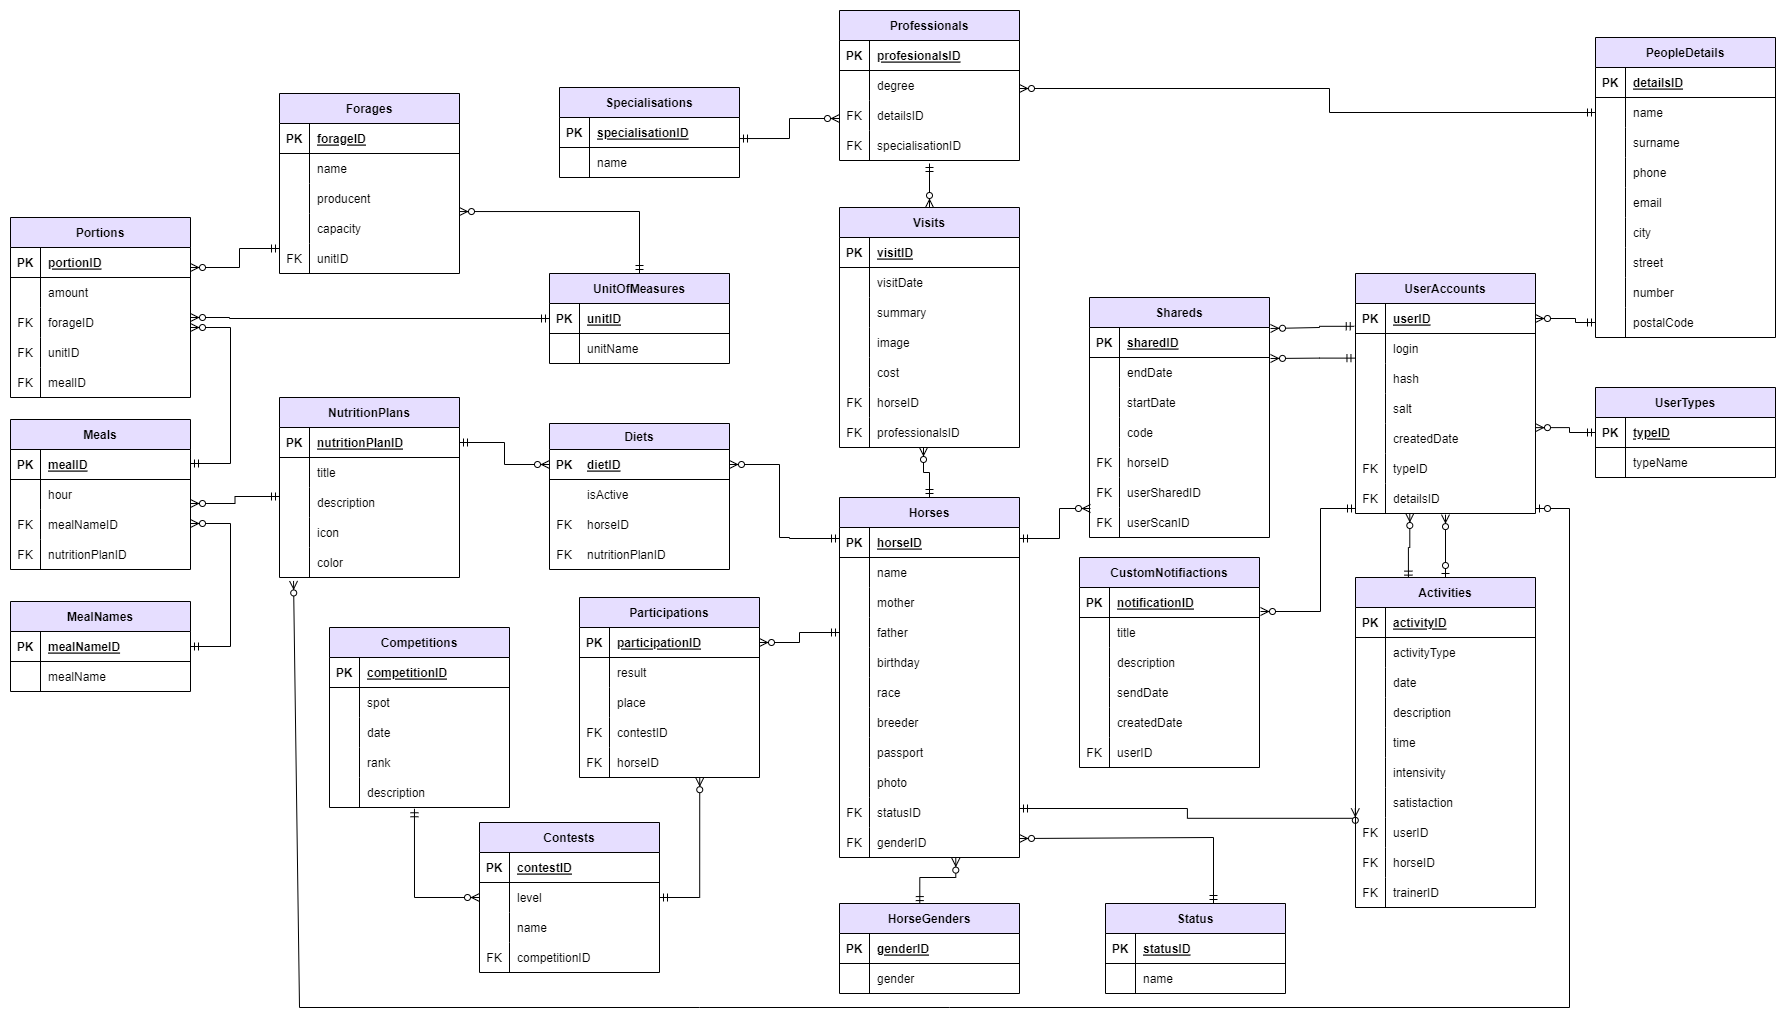
\includegraphics[scale=0.35, angle=-90]{DiagramLogiczny}
	\caption{Logiczny schemat bazy danych}
	\textit{Źródło: Opracowanie własne}
	\label{DiagramLogiczny}
\end{figure}
\newpage
\section{Model fizyczny}
Po stworzeniu logicznego modelu bazy danych, należy przetransformować go w model fizyczny. Model fizyczny jest to model bazy danych dostosowany do konkretnej bazy. Aby z relacji stworzyć tabele należy dostosować nazwy tabel i atrybutów oraz dopasować do atrybutów odpowiedni typy danych charakterystyczny dla wybranej bazy. Diagram fizyczny bazy danych znajduje się na rysunku rys. \ref{DiagramFizyczny}. Po zaprojektowaniu tabel można sporządzić skrypty tworzące bazę danych i tabele widoczne na listingu \ref{DatabaseCreate}.
\begin{lstlisting}[ language=SQL, 
					caption={Fragment skryptu tworzącego bazę danych i tabele},
					label={DatabaseCreate}]				
	-- Tworzenie bazy danych
	CREATE DATABASE HorseTracking;
	
	-- Uzywanie nowo utworzonej bazy danych
	USE HorseTracking;
	
	--Tworzenie tabel
	CREATE TABLE UserTypes (
	typeID INT NOT NULL IDENTITY(1,1) PRIMARY KEY,
	typeName varchar(20) NOT NULL)
	
	CREATE TABLE PeopleDetails (
	detailID INT NOT NULL IDENTITY(1,1) PRIMARY KEY,
	name varchar(40) NULL,
	surname varchar(40) NOT NULL,
	phone varchar(20) NULL,
	email varchar(320) NULL,
	city varchar(200) NULL,
	street varchar(90) NULL,
	number varchar(10) NULL,
	postalCode varchar(10) NULL)
\end{lstlisting}


\begin{figure}[H]
	\centering
	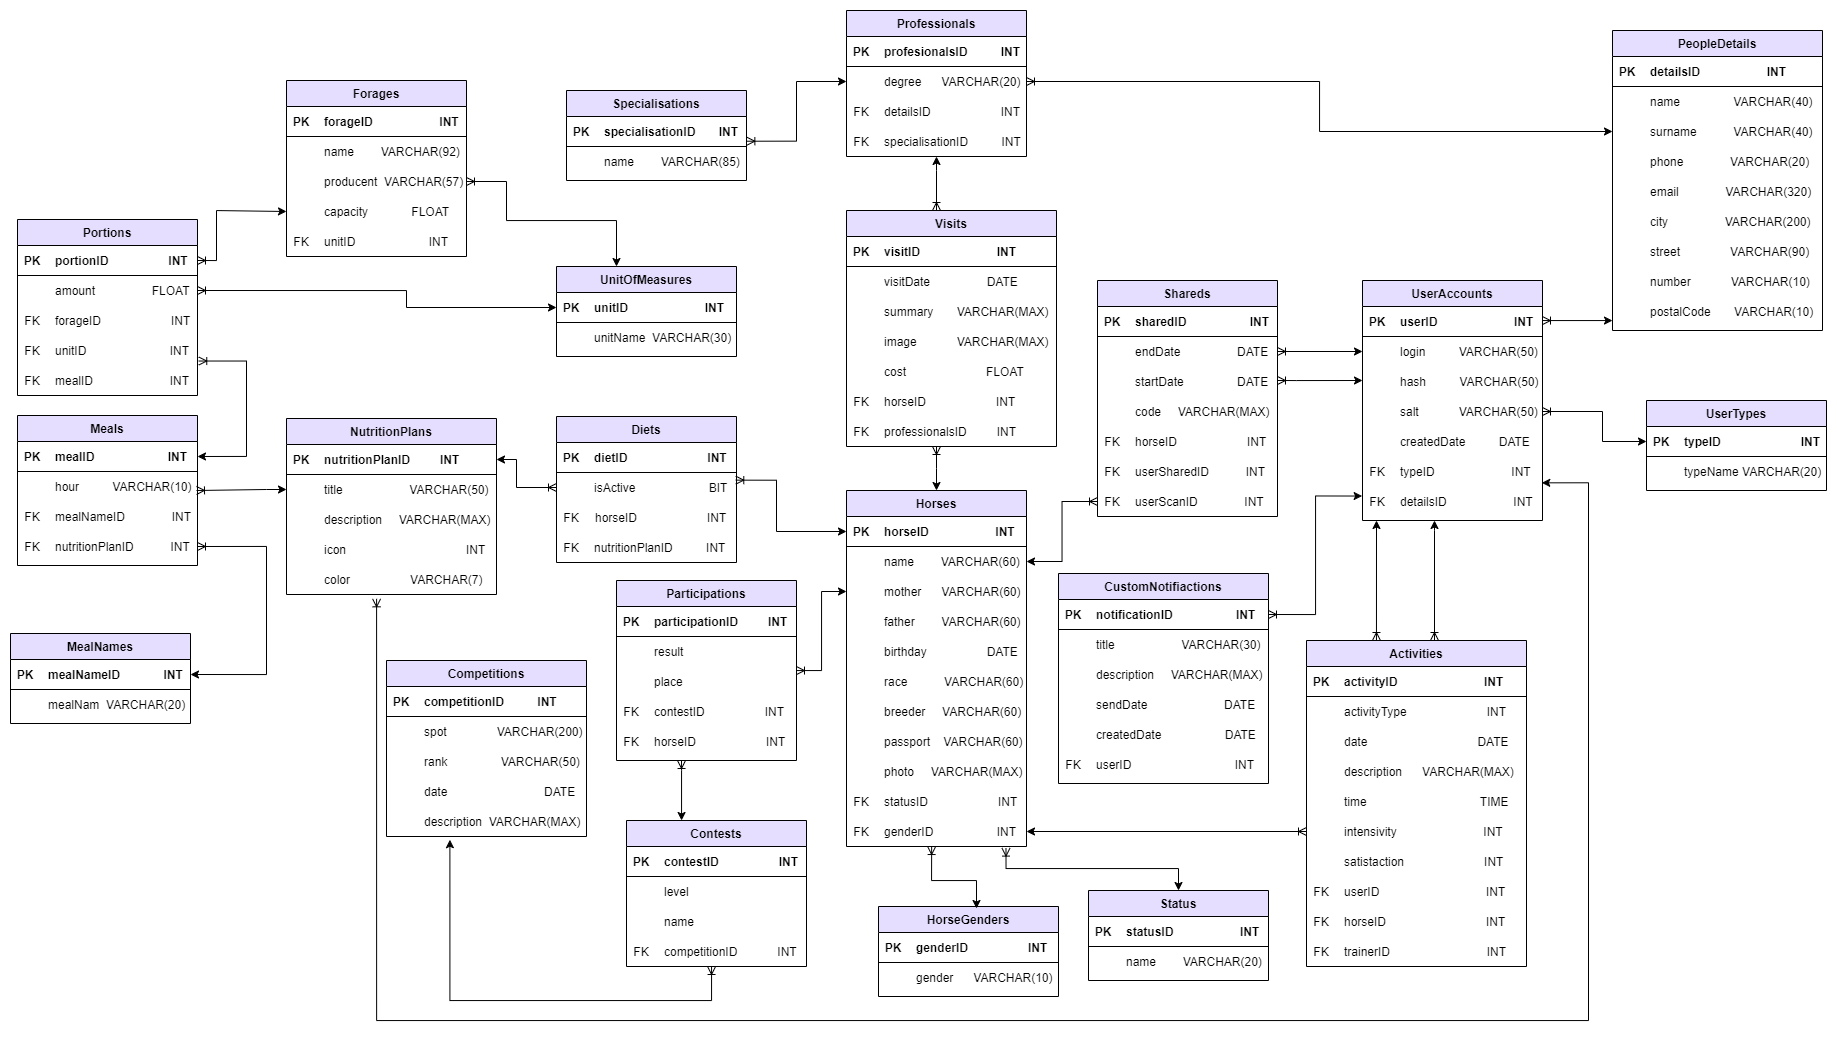
\includegraphics[scale=0.32, angle=-90]{DiagramFizyczny}
	\caption{Fizyczny schemat bazy danych}
	\textit{Źródło: Opracowanie własne}
	\label{DiagramFizyczny}
\end{figure}
\chapter{Projekt systemu}
\section{Model projektowanego systemu}
W tym rozdziale przedstawiony zostanie model projektowanego systemu. Zaprezentowane zostaną przykładowe diagramy aktywności, stanu, klas oraz sekwencji. Przedstawiona zostanie także architektura aplikacji oraz wykorzystane wzorce projektowe.

\subsection{Architektura aplikacji}
Jaka baza jakie połączenie itp.
\subsubsection{Model architektoniczny MVVM}
Jako model architektoniczny aplikacji mobilnej wybrano model MVVM, ponieważ jest on dedykowany aplikacją tego typu. W aplikacji desktopowej również został wybrany ten model ze względu na łatwość jego obsługi oraz wygodną implementacje w WPF, który wspiera data binding.
 
Wzorzec Model-View-ViewModel (MVVM) oddziela logikę i prezentacje aplikacji od interfejsu przeznaczonego dla użytkownika. Dzięki tej separacji można rozwiązać wiele problemów z zaprogramowaniem aplikacji. Pomaga ona także w testowaniu, konserwacji oraz rozwoju.\cite{MVVMmicLearn}
\begin{figure}[H]
	\centering
	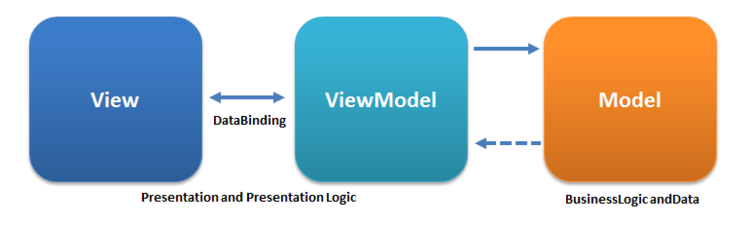
\includegraphics[scale=0.6]{MVVMPattern}
	\caption{Diagram przedstawiający architekturę MVVM }
	\textit{Źródło: \cite{mvvmpattern}}
	\label{MVVM}
\end{figure}
Jak można zobaczyć na rysunku \ref{MVVM} "View", czyli widok naszej aplikacji odpowiada za to co widzi użytkownik, za wszelkie struktury, układ elementów na ekranie oraz ich wygląd. "ViewModel", czyli model naszego widoku odpowiada za logikę aplikacji. To w nim zapisane są wszystkie komendy oraz metody. "ViewModel" powiadamia widok o wszelkich zmianach jest on odpowiedzialny za aktualizacje modeli. "Model" to klasa, która hermetyzuje dane aplikacji. Zawiera on dane reproezentujące logikę biznesową oraz obiekty transferu danych (DTO). Dzięki zastosowaniu MVVM model i widok są od siebie całkowicie niezależne. \cite{MVVMmicLearn}
Zalety korzystania z MVVM:
\begin{itemize}
	\item ułatwia tworzenie testów jednostkowych niezależnych od widoku. 
	\item interfejs użytkownika może być implementowany niezależnie od modelu. 
	\item wiele programistów może pracować na jednej aplikacji niezależnie. Widok możne być tworzony niezależnie od modelów i modelów widoku.
\end{itemize}
\subsubsection{Wykorzystane wzorce projektowe}
Podczas implementacji aplikacji desktopowej oraz mobilnej wykorzystano wzorce projektowe:
\begin{itemize}
\item \textbf{Dependency injection} - jest to wzorzec opierający się na paradygmacie "Odwróconego Sterowania". Polega on na tym, że zamiast wywoływania bibliotek przez kod programisty, to framoworki wywołują kod. Przez to że zachowanie między bibliotekami a kodem zostało odwrócone paradygmat nosi nazwę "Odwróconego sterowani".
Dzięki wzorcu projektowemu dependency injection możemy uniknąć ciągłego tworzenia nowych instancji serwisów oraz ciągłych zmian kodu w przypadku zmian w serwisach. Zajmuje się on wstrzykiwaniem potrzebnych zależności dzięki specjalnemu serwisowi.\cite{DI}
\item \textbf{Singleton} - jest to wzorzec dzięki któremu wiemy, że istnieje tylko jeden obiekt z danego rodzaju. Korzystając z tego wzorca wiemy, że np. dany serwis ma tylko jedną instancje z której stale korzystamy. Wzorzec ten ma zalety ale także wady, ponieważ ogranicza nam tworzenie testów jednostkowych oraz modularność kodu.
\end{itemize}
\subsubsection{Entity Framework}
Entity Framework to maper relacji obiektów, dzięki któremu można utworzyć warstwę dostępu do danych za pomocą .Net i dowolnej bazy danych działającej lokalnie bądź w chmurze. Obsługuje ono zapytania LINQ, aktualizacje, migracje oraz śledzenie zmian. Dzięki niemu możemy z łatwością łączyć aplikację z bazą danych i wykonywać na niej wszelkie operacje. \cite{EntityFramework}
\subsection{Diagramy UML}
Diagramy UML stanowią kluczowy element procesu projektowania aplikacji, pozwalając na graficzną reprezentację struktury, zachowań oraz relacji między różnymi częściami systemu.
\subsubsection{Diagramy stanów}
\begin{figure}[H]
	\centering
	\includegraphics[scale=0.8]{DiagramStanuKoń}
	\caption{Diagram stanu - koń}
	\textit{Źródło: Opracowanie własne}
	\label{DiagramStanuKoń}
\end{figure}
\subsubsection{Diagramy aktywności}
\begin{figure}[H]
	\centering
	\caption{Diagram aktywności logowanie}
	\textit{Źródło: Opracowanie własne}
	\label{DiagramAktywnościLogowanie}
\end{figure}
\subsubsection{Diagram klas}
\begin{figure}[H]
	\centering
	\caption{Fragment diagramu klas}
	\textit{Źródło: Opracowanie własne}
	\label{DiagramKlas}
\end{figure}
\subsubsection{Diagram sekwencji}
Diagram sekwencji pozwala na zaprezentowanie w sposób graficzny interakcji między obiektami, przy czym każda interakcja jest umieszczona w czasie. W aplikacji wiele interakcji można zobrazować za pomocą diagramu sekwencji. Jako przykład na poniższym diagramie (rys. \ref{DiagramSekwencjiUdostępnianie}) przedstawione zostało udostępnianie konia. 
\begin{figure}[H]
	\centering
	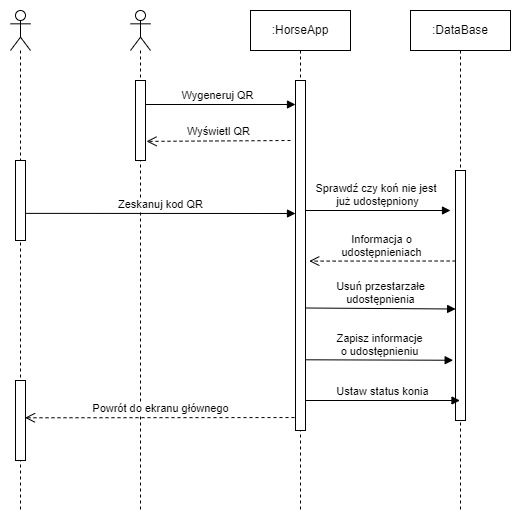
\includegraphics[scale=0.8]{DiagramSekwencjiUdostępnianie}
	\caption{Diagram sekwencji - udostępnianie koni}
	\textit{Źródło: Opracowanie własne}
	\label{DiagramSekwencjiUdostępnianie}
\end{figure}

\section{Wybrane aspekty implementacyjne}
W tym rozdziale przedstawione zostały wybrane fragmenty implementacji aplikacji mobilnej oraz desktopowej. Zaprezentowana została implementacja architektury aplikacji oraz wzorce projektowe przedstawione wcześniej. Przedstawione zostaną także niektóre z nuggetów opisane wcześniej oraz inne ciekawe aspekty implementacji.
\subsubsection{Implementacja architektury MVVM}
W aplikacji mobilnej oraz desktopowej zastosowano model architektoniczny MVVM. Implementacja modelu odbywa się poprzez zdefiniowanie DataContext jako odpowiedni view model co możemy zauważyć w listingu \ref{XamlFragmentMVVM}. Listing ten przedstawia fragment pliku xaml, w którym definiujemy paczki i zależności. W 8 linii listingu widzimy zdefiniowanie DataContext jako NutritionPageModel. \\
\begin{lstlisting}[language=C, caption={Fragment kodu xaml},
	label={XamlFragmentMVVM}]		
<Page x:Class="HorseTrackingDesktop.Pages.MainPage.NutritionPage"
xmlns="http://schemas.microsoft.com/winfx/2006/xaml/presentation"
xmlns:x="http://schemas.microsoft.com/winfx/2006/xaml"
xmlns:mc="http://schemas.openxmlformats.org/markup-compatibility/2006"
xmlns:d="http://schemas.microsoft.com/expression/blend/2008"
xmlns:main="clr-namespace:HorseTrackingDesktop.PageModel.Main"
xmlns:converter ="clr-namespace:HorseTrackingDesktop.Converters"
d:DataContext="{d:DesignInstance Type=main:NutritionPageModel}"
mc:Ignorable="d"
d:DesignHeight="450" d:DesignWidth="800"
Title="NutritionPage">
\end{lstlisting}
Dodatkowo, aby przypisać odpowiednie metody do eventu ładowania podpięto także DataContext w pliku .cs widoku (patrz listing \ref{CSFragmentMVVM}).  View model został wstrzyknięty za pomocą Dependency Incjection, a następnie przypisany pod DataContext. \\
\begin{lstlisting}[ caption={Podpięcie DataContext w pliku .cs},
	label={CSFragmentMVVM}]	
namespace HorseTrackingDesktop.Pages.MainPage
{
	public partial class NutritionPage : Page
	{
		private NutritionPageModel? pageModel;
			
		public NutritionPage()
		{
			InitializeComponent();
			pageModel = StartUp.ServiceProvider?.GetService<NutritionPageModel>();
			DataContext = pageModel;
			if (pageModel != null)
			{
				Loaded += async (s, e) => await pageModel.GetPlans();
			}
		}
	}
}
\end{lstlisting}
Można zauważyć, że w pliku widocznym na listingu \ref{CSFragmentMVVM} nie ma żadnych metod dotyczących funkcjonalności aplikacji jest to część implementacji MVVM. Dzięki temu, że podpięty został ViewModel możemy tam umieścić wszystkie te metody a tym samy oddzielić je od widoku. \\
\begin{lstlisting}[ caption={Podpięcie DataContext w pliku .cs},
	label={CSFragmentMVVM}]	
	namespace HorseTrackingDesktop.Pages.MainPage
	{
		public partial class NutritionPage : Page
		{
			private NutritionPageModel? pageModel;
			
			public NutritionPage()
			{
				InitializeComponent();
				pageModel = StartUp.ServiceProvider?.GetService<NutritionPageModel>();
				DataContext = pageModel;
				if (pageModel != null)
				{
					Loaded += async (s, e) => await pageModel.GetPlans();
				}
			}
		}
	}
\end{lstlisting}
Dzięki użyciu tej architektury można uniknąć powtarzania tego samego kodu. Możemy używać jednego ViewModelu do obsługi wielu widoków. W aplikacji zostało to użyte wiele razy, większość widoków dodawania, edytowania oraz szczegółów danego komponentu implementują ten sam ViewModel.
\subsubsection{INotifyPropertyChanged}
ViewModel musi informować widok o zmianach w różnych zmiennych w nim zaimplementowanych, aby mógł to robić zaimplementowany został interfejs INotifyPropertyChanged. Każdy ViewModel musi implementować ten interfejs, dlatego utworzono klasę bazową (patrz listnig \ref{BaseClass}), w której został on zaimplementowany, a wszystkie view modele mogą po niej dziedziczyć. \\
\begin{lstlisting}[ caption={Klasa bazowa view modeli},
	label={BaseClass}]	
 public class BaseViewModel : INotifyPropertyChanged
{
	protected bool SetProperty<T>(ref T backingStore, T value,
	[CallerMemberName] string propertyName = "",
	Action onChanged = null)
	{
		if (EqualityComparer<T>.Default.Equals(backingStore, value))
		return false;
		
		backingStore = value;
		onChanged?.Invoke();
		OnPropertyChanged(propertyName);
		return true;
	}
	
	public event PropertyChangedEventHandler PropertyChanged;
	
	protected void OnPropertyChanged([CallerMemberName] string propertyName = "")
	{
		var changed = PropertyChanged;
		if (changed == null)
		return;
		
		changed.Invoke(this, new PropertyChangedEventArgs(propertyName));
	}
}
\end{lstlisting}
W klasie tej zaimplementowano łatwiejszy dostęp do wywołania eventu \textbf{PropertyChangedEventArgs} poprzez wywołanie metody \textbf{OnPropertyChanged}(argument), gdzie jako argument podajemy nazwę zmiennej. Zaimplementowano także metodę SetProperty która pozwala na łatwe przypisywanie wartości do zmiennych z jednoczesną aktualizacją ich w widoku użytkownika.
\subsubsection{Dependency Injection}
W aplikacji użyto Dependency Injection do wstrzykiwania zależności do viewModeli i serwisów. W celu implementacji użyty został nugget Microsoft.Extensions.DependencyInjection w aplikacji mobilnej oraz desktopowej. Utworzono klasę statyczną StartUp.cs (patrz listing \ref{StartUp}) w której zaimplementowano serwis obsługujący wstrzykiwanie.\\
\begin{lstlisting} [ caption={Klasa StartUp},
	label={StartUp}]	
public static class Startup
{
	public static IServiceProvider ServiceProvider { get; set; }
	
	public static IServiceProvider Init()
	{
		var serviceProvider = new ServiceCollection()
		.ConfigureServices()
		.ConfigureViewModels()
		.BuildServiceProvider();
		
		ServiceProvider = serviceProvider;
		
		return serviceProvider;
	}
}
\end{lstlisting}	
Metody konfigurujące serwisy oraz view modele zostały zaimplementowane w klasie DependencyInjectionContainer widoczną na listingu \ref{DependencyInjectionContainer}.\\
\begin{lstlisting} [ caption={Klasa DependencyInjectionContainer}, label={DependencyInjectionContainer}]	
 public static class DependencyInjectionContainer
{
	public static IServiceCollection ConfigureServices(this IServiceCollection services)
	{
		services.AddSingleton<IUserService, UserService>();
		services.AddSingleton<IAppState, AppState>();
		:
		return services;
	}
	
	public static IServiceCollection ConfigureViewModels(this IServiceCollection services)
	{
		services.AddTransient<LoginViewModel>();
		services.AddSingleton<BaseViewModel>();
		:
		return services;
	}
}
\end{lstlisting}
Można zauważyć, że serwisy zostały zainicjowane jako Singletony, ponieważ potrzebujemy tylko jedną ich instancje, natomiast viewModele jako transient, ponieważ przy każdym ich użyciu chcemy mieć ich nową instancje.
Dzięki dependency injection nie trzeba ręcznie tworzyć wszystkich zależności i zależności do ich zależności. Można w łatwy sposób w konstruktorze wstrzyknąć wszystko co jest potrzebne (patrz. listing \ref{DIConstruktor}).
\begin{lstlisting} [ caption={Wstrzykiwanie zależności w konstruktorze}, label={DIConstruktor}]	
public ActivityViewModel(IActivityService activityServices, IAppShellRoutingService appShellRoutingService,
IAppState appState, IHorseService horseService)
{
	_activityServices = activityServices;
	_appShellRoutingService = appShellRoutingService;
	_appState = appState;
	_horseService = horseService;
	:
}
\end{lstlisting}
\subsubsection{Command i RelayCommand}
Większość funkcjonalności z aplikacji mobilnej została zaimplementowana jako komendy używając klasy Command, co można zobaczyć na poniższym listingu \ref{Command}.
\begin{lstlisting} [ caption={Użycie komend}, label={Command}]	
public LoginViewModel(IUserService userService, IAppState appState, IHorseService horseService, IShareHorseServices shareHorseServices)
{
	_userService = userService;
	_appState = appState;
	_horseService = horseService;
	_shareHorseServices = shareHorseServices;
	
	LoginCommand = new Command(() =>
	{
		if (string.IsNullOrWhiteSpace(ReadedLogin) && string.IsNullOrWhiteSpace(ReadedPassword))
		return;
		var hashedPassword = ReadedPassword;
		var user = _userService.GetUser(ReadedLogin, hashedPassword);
		if (user == null)
		{
			IncorrectData();
			return;
		}
		_appState.CurrentUser = user;
		GoToTheApp();
	});
}
\end{lstlisting}
Zaś w aplikacji desktopowej użyto RelayCommand z paczki nuggetowej (patrz listing \ref{RelayCommand})
\begin{lstlisting} [ caption={Użycie RelayCommand}, label={RelayCommand}]	
[RelayCommand]
public async Task GoToAddPlan()
{
	new AddNutritionView().ShowDialog();
	await GetPlans();
}
\end{lstlisting}
\subsubsection{QRCode}
W aplikacji jest możliwość udostępniania koni między użytkownikami. Można to zrobić przez zwykłą wyszukiwarkę lub szybciej za pomocą kodu QR. Do udostępniania przez QR zaprojektowano dwa widoki, jeden ze skanerem (patrz listing \ref{QRScan}), oraz drugi umożliwiający generacje kodu. 

Scanner zdefiniowany jest w 12 linijce listingu \ref{QRScan}. Skaner skanuje tylko jeśli zmienna IsScanning ustalona jest na true. Po zeskanowaniu odpala się event \textbf{OnScanResult}, gdzie dostępny jest zeskanowany tekst. \\
\begin{lstlisting} [ caption={Skaner kodów QR}, label={QRScan}]	
<ContentPage xmlns="http://xamarin.com/schemas/2014/forms"
xmlns:x="http://schemas.microsoft.com/winfx/2009/xaml"
x:Class="HorseTrackingMobile.Views.ScanHorseView"
xmlns:zxing="clr-namespace:ZXing.Net.Mobile.Forms;assembly=ZXing.Net.Mobile.Forms"
xmlns:zxingcommon="clr-namespace:ZXing.Common;assembly=zxing.portable"
xmlns:viewmodels="clr-namespace:HorseTrackingMobile.ViewModels"
x:DataType="viewmodels:ScanHorseViewModel"
Shell.TabBarIsVisible="False"
Shell.FlyoutBehavior="Disabled">
<ContentPage.Content>
	<StackLayout>
		<zxing:ZXingScannerView OnScanResult='ZXingScannerView_OnScanResult'
								IsScanning="{Binding IsScanning}" />
	</StackLayout>
</ContentPage.Content>
</ContentPage>
\end{lstlisting}
Aby użytkownik mógł zeskanować kod QR, wcześniej inny osoba musi wygenerować go w aplikacji. Aby to zrobić przygotowany został widok z generatorem kodów QR przedstawiony na listingu \ref{QRGen}. W widoku tym możliwe jest nie tylko same generowanie, lecz także wybranie udostępnianego konia oraz daty ważności udostępnienia. Po wybraniu obu tych wartości widoczny jest QR kod gotowy do zeskanowania przez innych użytkowników. Generator kodów QR podobnie jak skaner pochodzi z paczki ZXing, zadeklarowanej w 3 linijce listingu \ref{QRGen}. Koń na raz może być udostępniony tylko jednej osobie, więc po zeskanowaniu kod staje nie ważny. \\
\begin{lstlisting} [ caption={Wyświetlanie kodów QR}, label={QRGen}]	
<ContentPage xmlns="http://xamarin.com/schemas/2014/forms"
xmlns:x="http://schemas.microsoft.com/winfx/2009/xaml"
xmlns:zxing="clr-namespace:ZXing.Net.Mobile.Forms;assembly=ZXing.Net.Mobile.Forms"
xmlns:viewmodels="clr-namespace:HorseTrackingMobile.ViewModels"
xmlns:zxingcommon="clr-namespace:ZXing.Common;assembly=zxing.portable"
x:DataType="viewmodels:ShareHorseViewModel"
x:Class="HorseTrackingMobile.Views.ShareHorseView"
Shell.TabBarIsVisible="False"
Shell.FlyoutBehavior="Disabled">
<ContentPage.Content>
<StackLayout Margin="30,50">
<Label Text="Wybierz konia: " />
<Picker SelectedItem="{Binding SelectedHorse}"
ItemsSource="{Binding Horses}"
ItemDisplayBinding="{Binding Name, Mode=TwoWay}" />
<Label Text="Wybierz date:" />
<DatePicker Date="{Binding EndDate, Mode=TwoWay}" MinimumDate="{Binding DateNow}" />
<zxing:ZXingBarcodeImageView BarcodeFormat="QR_CODE" BarcodeValue="{Binding BarcodeValue}" WidthRequest="500" HeightRequest="500">
<zxing:ZXingBarcodeImageView.BarcodeOptions>
<zxingcommon:EncodingOptions Height="500" Width="500" />
</zxing:ZXingBarcodeImageView.BarcodeOptions>
</zxing:ZXingBarcodeImageView>
</StackLayout>
</ContentPage.Content>
</ContentPage>
\end{lstlisting}
\subsubsection{Kodowanie i odkodowanie}
Informacje o udostępnieniu przekazywane w kodach QR są szyfrowane, aby nie możliwe było podrobienie kodu i przejęcie czyiś koni. Informacja przekazywana w kodzie zawiera id konia oraz datę ważności udostępnienia. Gdyby nie była ona zaszyfrowana inny użytkownik mógłby z łatwością wygenerować kody QR pozwalające na udostępnianie różnych koni. Aby zapobiec takiemu nie pożądanemu zjawisku wprowadzono szyfrowanie i odszyfrowanie tekstu z kodu QR (patrz listing \ref{EncodeDecode}). \\
\begin{lstlisting} [ caption={Kodowanie i odkodowanie}, label={EncodeDecode}]	
 private byte[] EncryptStringToBytes_Aes(string text, byte[] key, byte[] iv)
{
	using (var aesAlg = Aes.Create())
	{
		aesAlg.Key = key;		aesAlg.IV = iv;
		var encryptor = aesAlg.CreateEncryptor(aesAlg.Key, aesAlg.IV);
		using (var msEncrypt = new MemoryStream())
		{
			using (var csEncrypt = new CryptoStream(msEncrypt, encryptor, CryptoStreamMode.Write))
			{
				using (var swEncrypt = new StreamWriter(csEncrypt))
				{
					swEncrypt.Write(text);
				}
			}
			return msEncrypt.ToArray();
}}}
private string DecryptStringFromBytes_Aes(byte[] text, byte[] key, byte[] iv)
{
	using (var aesAlg = Aes.Create())
	{
		aesAlg.Key = key;		aesAlg.IV = iv;
		var decryptor = aesAlg.CreateDecryptor(aesAlg.Key, aesAlg.IV);
		using (var msDecrypt = new MemoryStream(text))
		{
			using (var csDecrypt = new CryptoStream(msDecrypt, decryptor, CryptoStreamMode.Read))
			{
				using (var srDecrypt = new StreamReader(csDecrypt))
				{
					return srDecrypt.ReadToEnd();
}}}}}
\end{lstlisting}
\subsubsection{Własne kontrolki}
Menu boczne dostępne w aplikacji desktopowej zostało stworzone z customowych kontrolek. Przyciski dostępne w menu to przyciski zapewniające dodatkowy routing do określonej strony oraz obrazek. Klasa w której została stworzona kontrolka (patrz listing \ref{navButton}) dziedziczy po klasie Button i wykorzystuje wiele jego funkcjonalności.\\

\begin{lstlisting} [ caption={Kontrolka NavigationButton}, label={navButton}]	
public class NavigationButton : Button
{
	static NavigationButton()	{
		DefaultStyleKeyProperty.OverrideMetadata(typeof(NavigationButton), new FrameworkPropertyMetadata(typeof(NavigationButton)));	}
	
	public NavigationButton()	{
		this.Template = (ControlTemplate)Application.Current.Resources["Template"];}
	
	public ImageSource ImageSource	{
		get { return (ImageSource)GetValue(ImageSourceProperty); }
		set { SetValue(ImageSourceProperty, value); }	}
	
	public static readonly DependencyProperty ImageSourceProperty = DependencyProperty.Register("ImageSource", typeof(ImageSource), typeof(NavigationButton), new PropertyMetadata(null));
	
	public Brush Highlight	{
		get { return (Brush)GetValue(HighlightProperty); }
		set { SetValue(HighlightProperty, value); }	}
	
	public static readonly DependencyProperty HighlightProperty = DependencyProperty.Register("Highlight", typeof(Brush), typeof(NavigationButton), new PropertyMetadata(null));
	
	public Uri Routing	{
		get { return (Uri)GetValue(RoutingProperty); }
		set { SetValue(RoutingProperty, value); }	}
	
	public static readonly DependencyProperty RoutingProperty = DependencyProperty.Register("Routing", typeof(Uri), typeof(NavigationButton), new PropertyMetadata(null));
}
\end{lstlisting}
\subsubsection{Konwertery}
W aplikacji desktopowej zastosowano dwa konwertery dotyczące widoczności obiektów w UI użytkownika. Jeden z nich konwertuje zmienną boolowską prawda/fałsz na odpowiedni enumerator widoczności, zaś drugi datę. Pierwszy z nich został przedstawiony na listingu \ref{converter}. \\
\begin{lstlisting} [ caption={Konwerter}, label={converter}]	
	public class BoolToVisibilityConverter : IValueConverter
	{
		public object Convert(object value, Type targetType, object parameter, CultureInfo culture)
		{
			if (value is bool boolValue && boolValue)
			{
				return Visibility.Visible;
			}
			else
			{
				return Visibility.Collapsed;
			}
		}
		
		public object ConvertBack(object value, Type targetType, object parameter, CultureInfo culture)
		{
			throw new NotSupportedException();
		}
	}
\end{lstlisting}
\subsubsection{Hash i salt}
\newpage
\chapter{Dokumentacja użytkownika}
\section{Aplikacja desktopowa}
Aplikacja desktopowa "HorseTracking" służy do zarządzania wizytami, żywieniem i zawodami. Można w niej obejrzeć także statystyki z aktywności oraz zawodów. W aplikacji tej dostępny jest także kalendarz z zapisanymi wszystkimi wydarzeniami. Po uruchomieniu użytkownikowi wyświetlony zostaje panel logowania. Każdy użytkownik, posiadający konto w aplikacji może się zalogować. Stworzenie konta, samodzielnie przez użytkownika nie jest możliwe.
\begin{figure}[H]
	\centering
	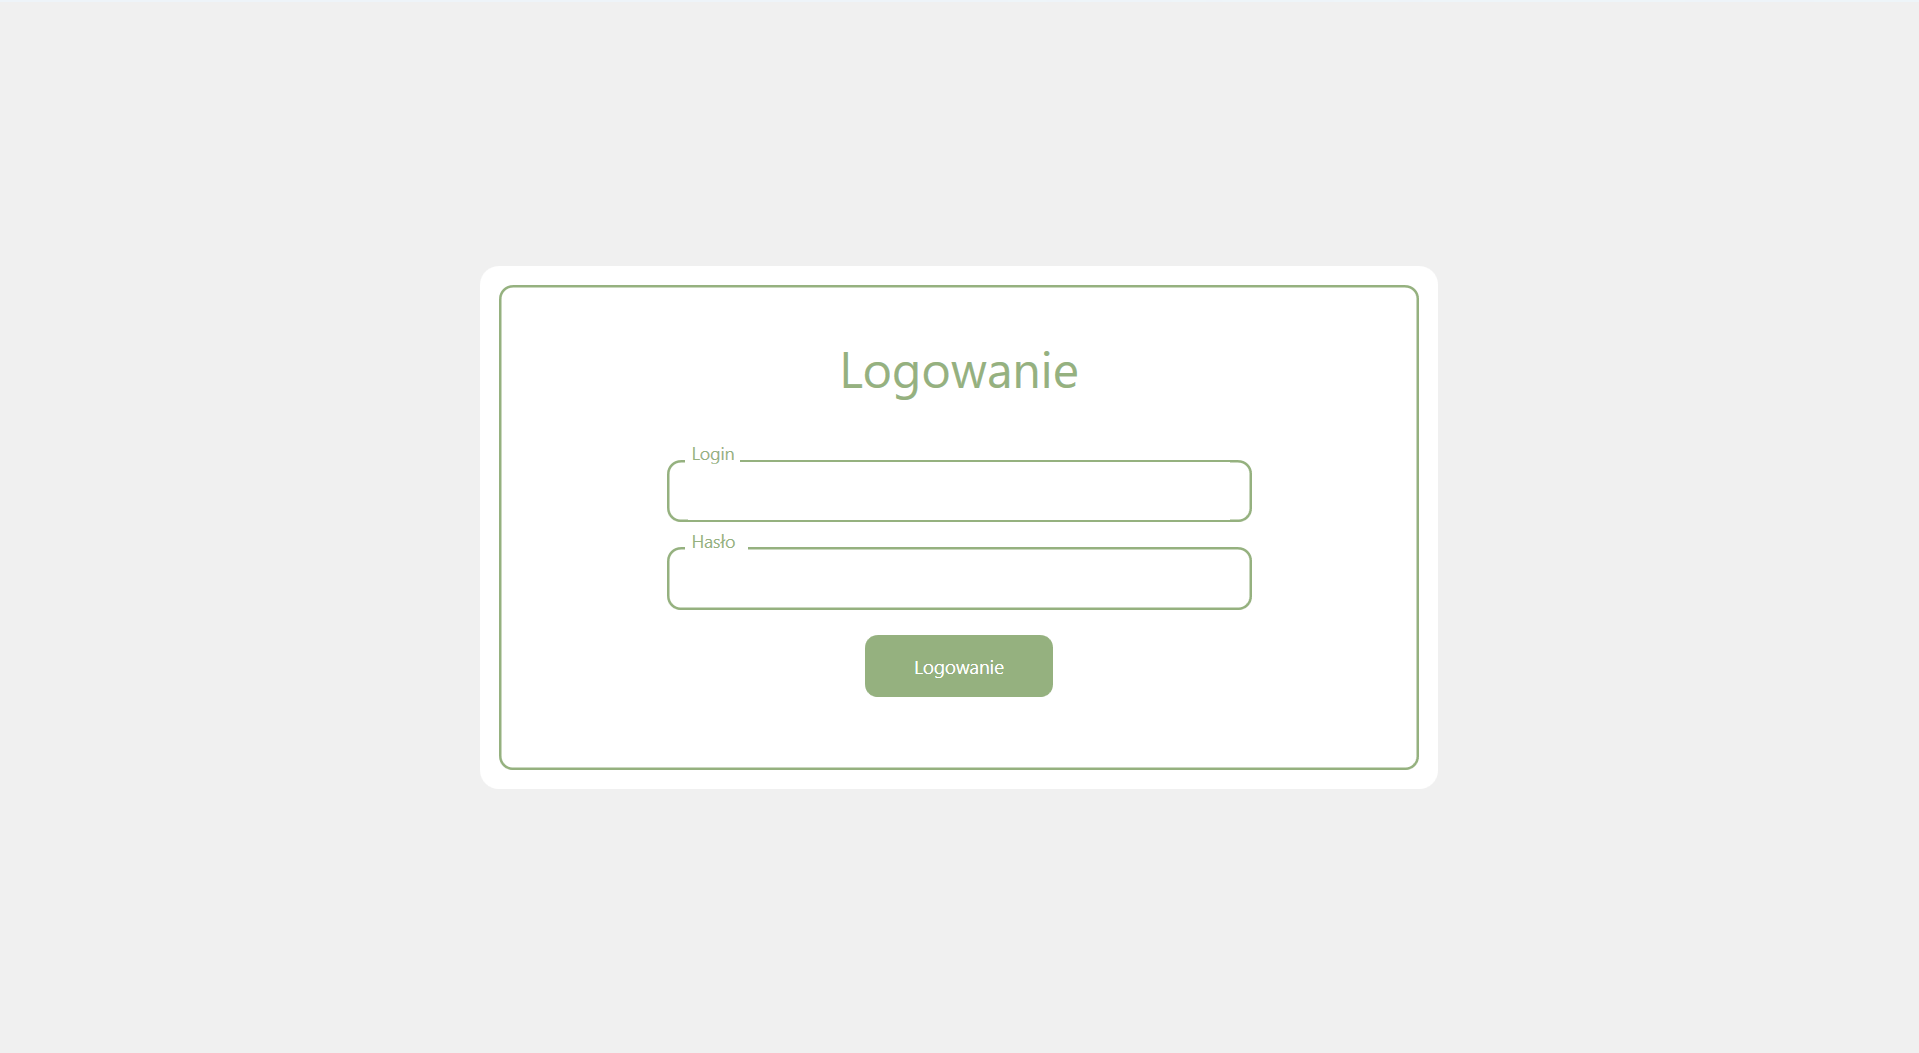
\includegraphics[scale=0.32]{Logowanie}
	\caption{Panel logowania}
	\textit{Źródło: Opracowanie własne}
	\label{Logowanie}
\end{figure}
Po zalogowaniu widoczna jest strona statystyk wraz z bocznym menu. 
\begin{figure}[H]
\centering
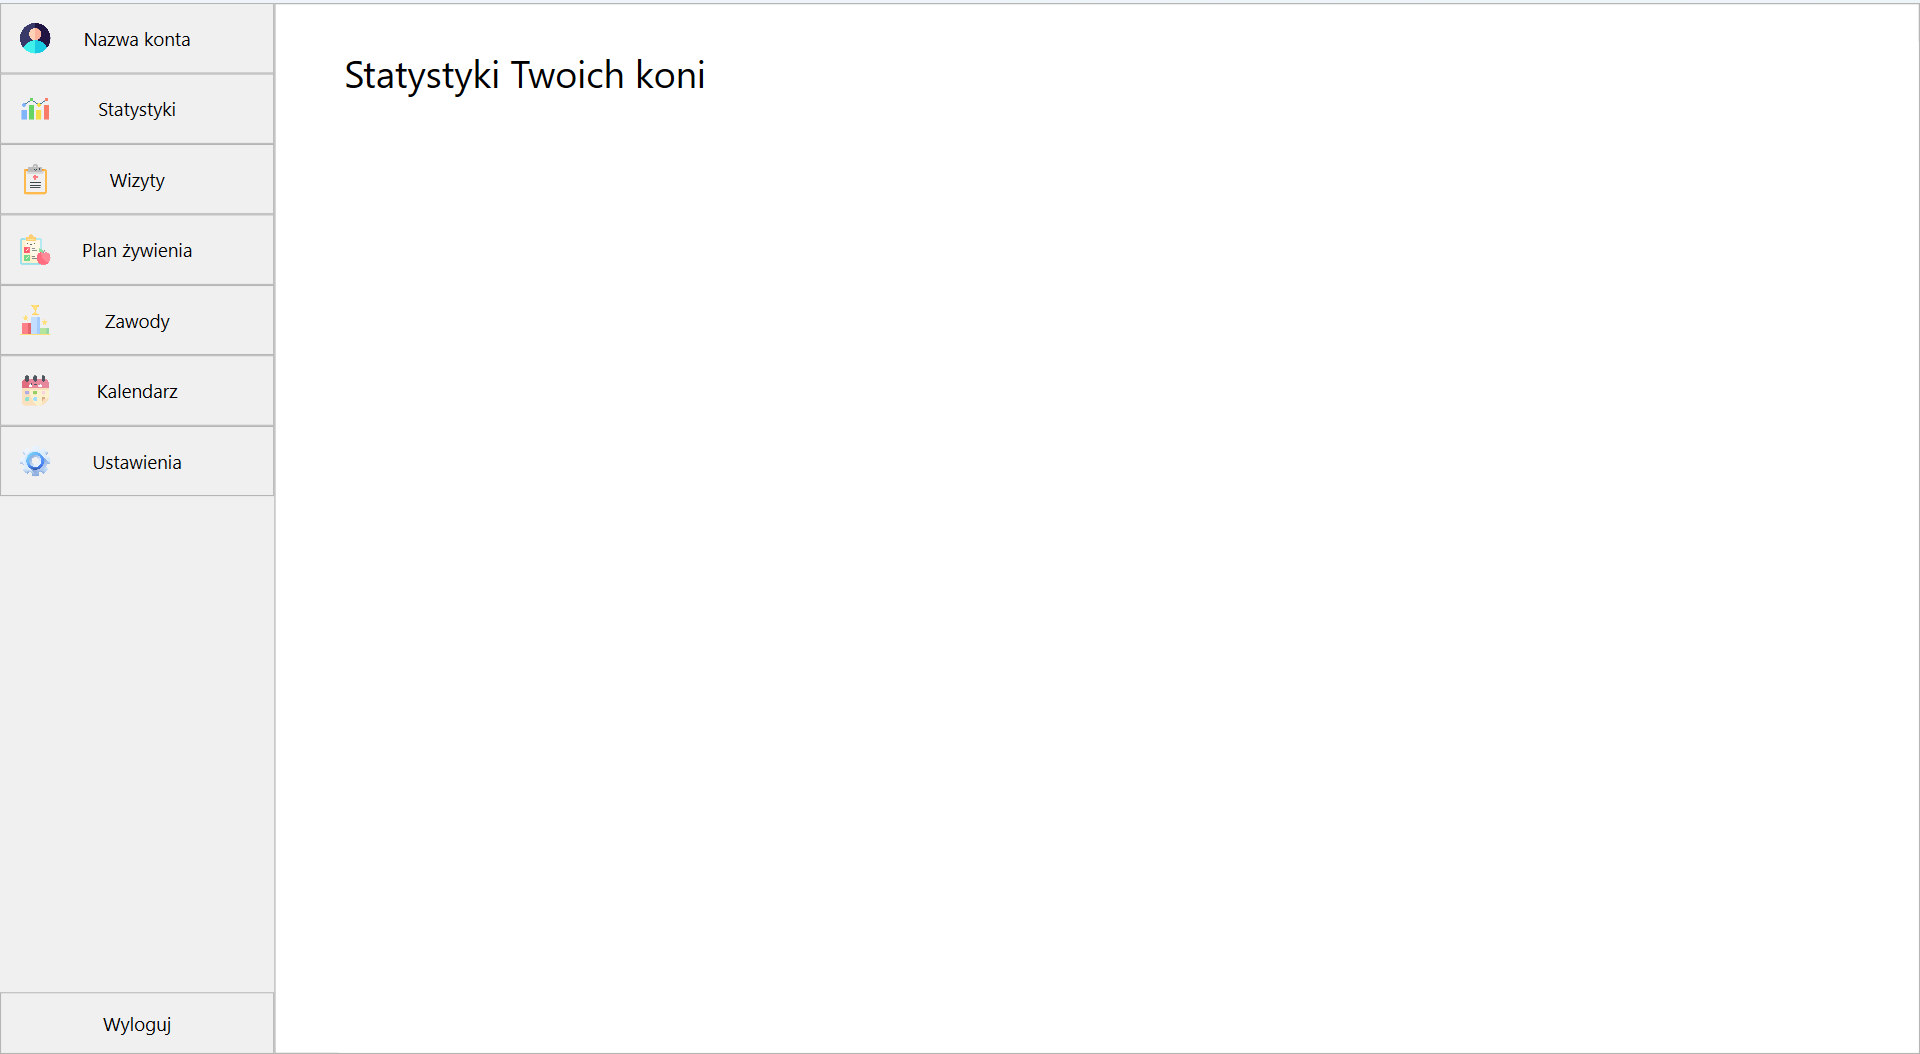
\includegraphics[scale=0.4]{Statystyki}
\caption{Strona statystyk}
\textit{Źródło: Opracowanie własne}
\label{Statystyki}
\end{figure}
Wśród statystyk w lewym górnym rogu widoczne jest miesięczne zestawienie aktywności jednego konia oraz w lewym dolnym wszystkich koni. .........(Dokończyć jak będzie więcej wiadomo)

\begin{figure}[H]
\centering
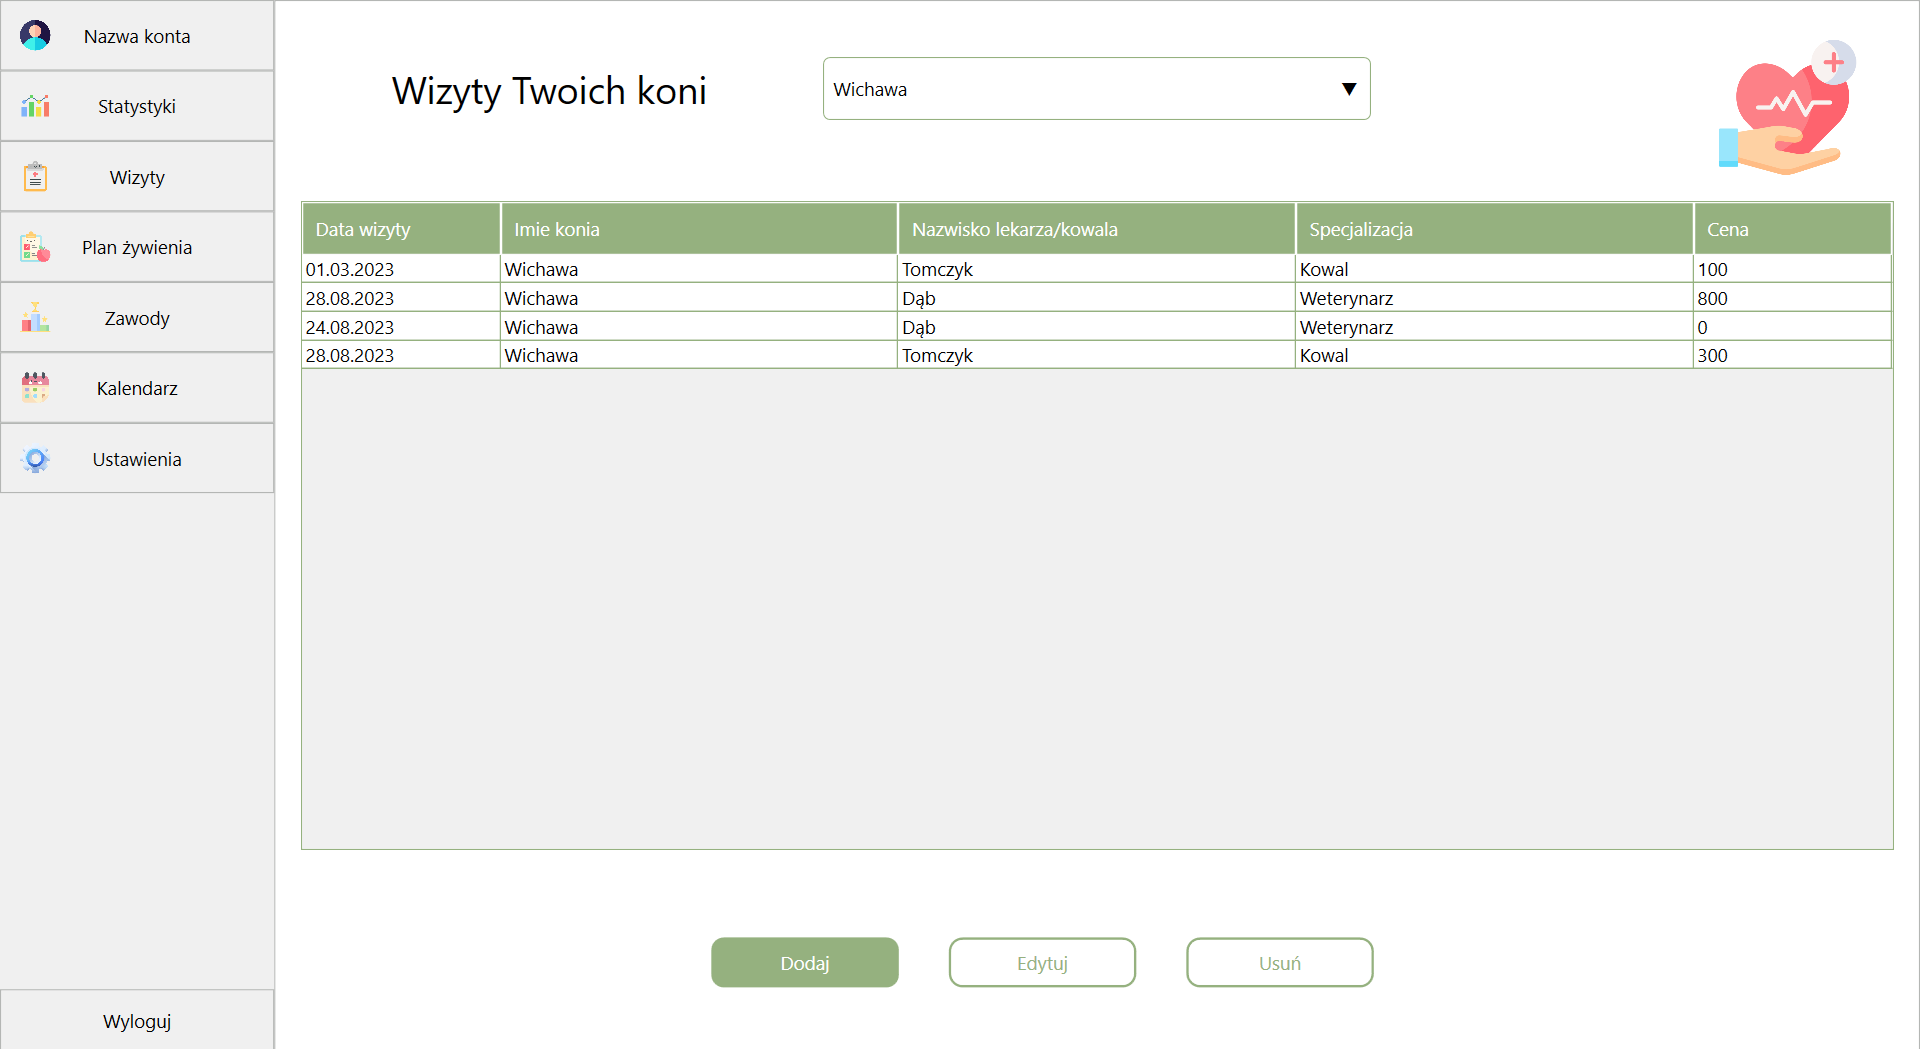
\includegraphics[scale=0.4]{Wizyty}
\caption{Strona wizyt}
\textit{Źródło: Opracowanie własne}
\label{Wizyty}
\end{figure}
Po wybraniu wizyt z menu bocznego można obejrzeć wizyty koni. Na górze ekranu widoczny jest pole, dzięki któremu możemy wybrać dla jakiego konia mają być wyświetlane wizyty. Wizyty wyświetlane są w tabeli, posegregowane według malejąco według daty jej odbycia. Na głównym ekranie występują jedynie skrócone informacje na temat wizyty. Dostępna jest data wizyty, imię konia który odbywał wizytę, nazwisko oraz specjalizacja lekarza lub kowala oraz cena wizyty. 

Szczegóły konkretnej wizyty można obejrzeć klikając dwa razy na wiersz w tabeli z informacjami o niej. Po kliknięciu pojawi się nowe okno (patrz rys. \ref{WizytyDetale}) na którym znajduje się nie tylko szczegółowy opis przebiegu wizyty, ale także zdjęcie z wizyty, wszelkie szczegółowe informacje dotyczące konia oraz osoby przeprowadzającej. Po obejrzeniu szczegółów można powrócić do okna głównego klikając przycisk "Wróć".
\begin{figure}
	\begin{center}
		\begin{minipage}{6cm}
			\centering
			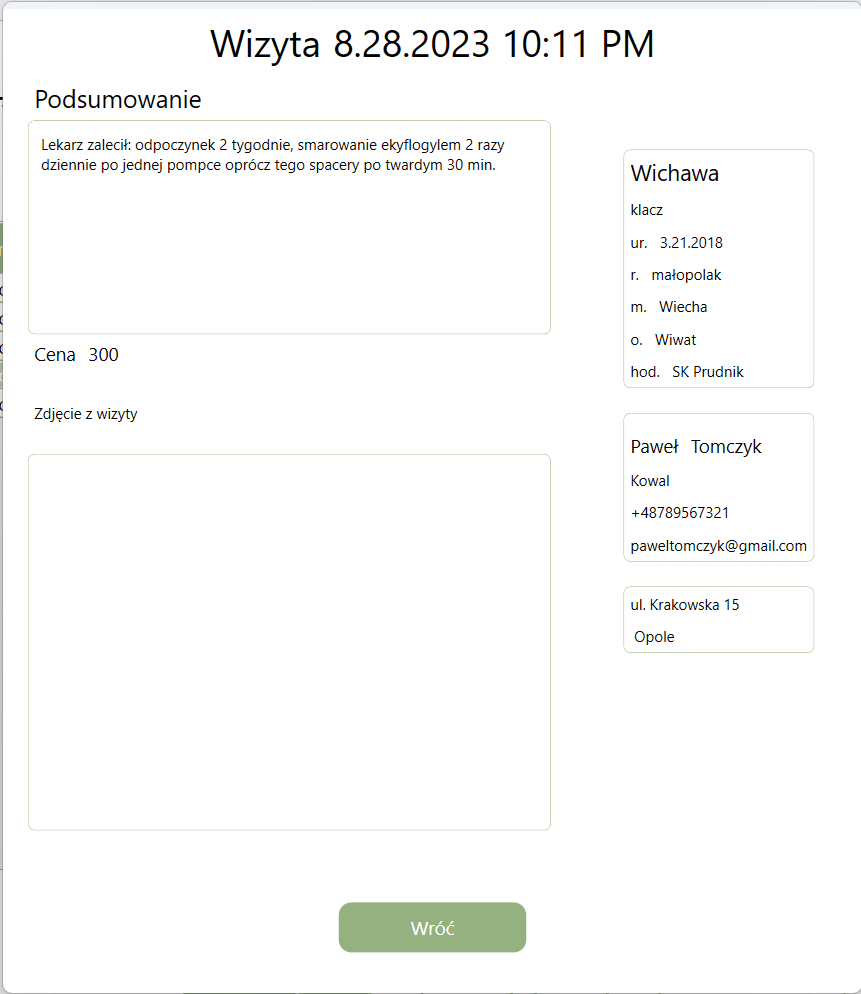
\includegraphics[scale=0.4]{wizytyDetale}
			\caption{Szczegóły wizyty}
			\textit{Źródło: Opracowanie własne}
			\label{WizytyDetale}
		\end{minipage}
		\hfil
		\begin{minipage}{6cm}
			\centering
			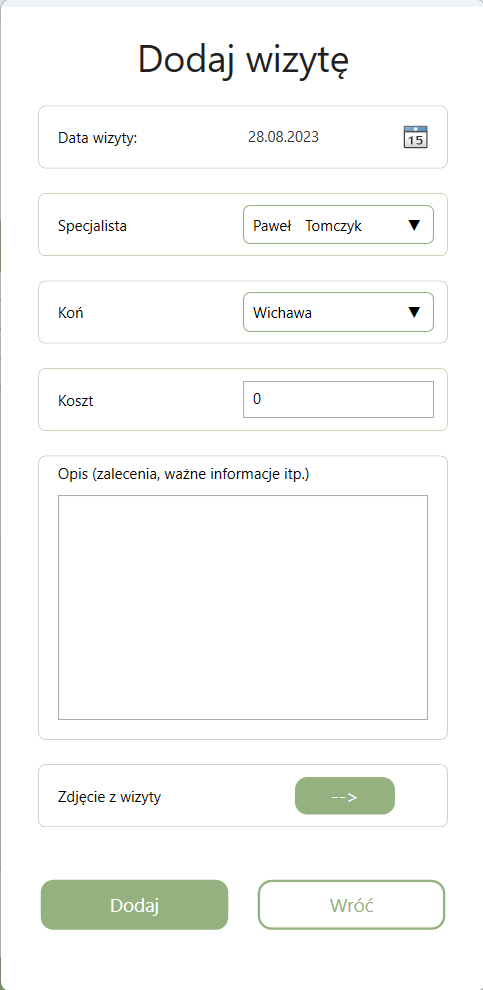
\includegraphics[scale=0.4]{dodajWizyte}
			\caption{Dodawanie wizyt}
			\textit{Źródło: Opracowanie własne}
			\label{DodajWizyty}
		\end{minipage}
	\end{center}
\end{figure}
Na dole głównego ekranu znajdują się trzy przyciski pozwalające na zarządzanie wizytami. Po kliknięciu przycisku dodaj otworzy się nowe okno pozwalające dodać nową wizytę (patrz rys.\ref{DodajWizyty}). W oknie tym możemy wybrać konia, lekarza oraz dodać opis wizyty i zapisać koszta z nią związane. Data wizyty automatycznie ustawiona jest na dzisiejszą, jednakże można ją dowolnie modyfikować. Oprócz przycisku "dodaj" dostępny jest także przycisk "edytuj". Przycisk ten pozwala na edycje obecnie zaznaczonej wizyty. Otwiera on to samo okno co przy dodawaniu, jednakże tym razem widok jest już wypełniony danymi. Ostatni z przycisków, przycisk "usuń" pozwala na usunięcie obecnie zaznaczonej wizyty. Na oknie dodawania wizyt dostępny jest przycisk dodania zdjęcia. Przycisk ten przenosi użytkownika na nowe okno, w którym możliwe jest wgranie zdjęcia z komputera i zapisanie go do bazy danych.

\begin{figure}[h]
	\centering
	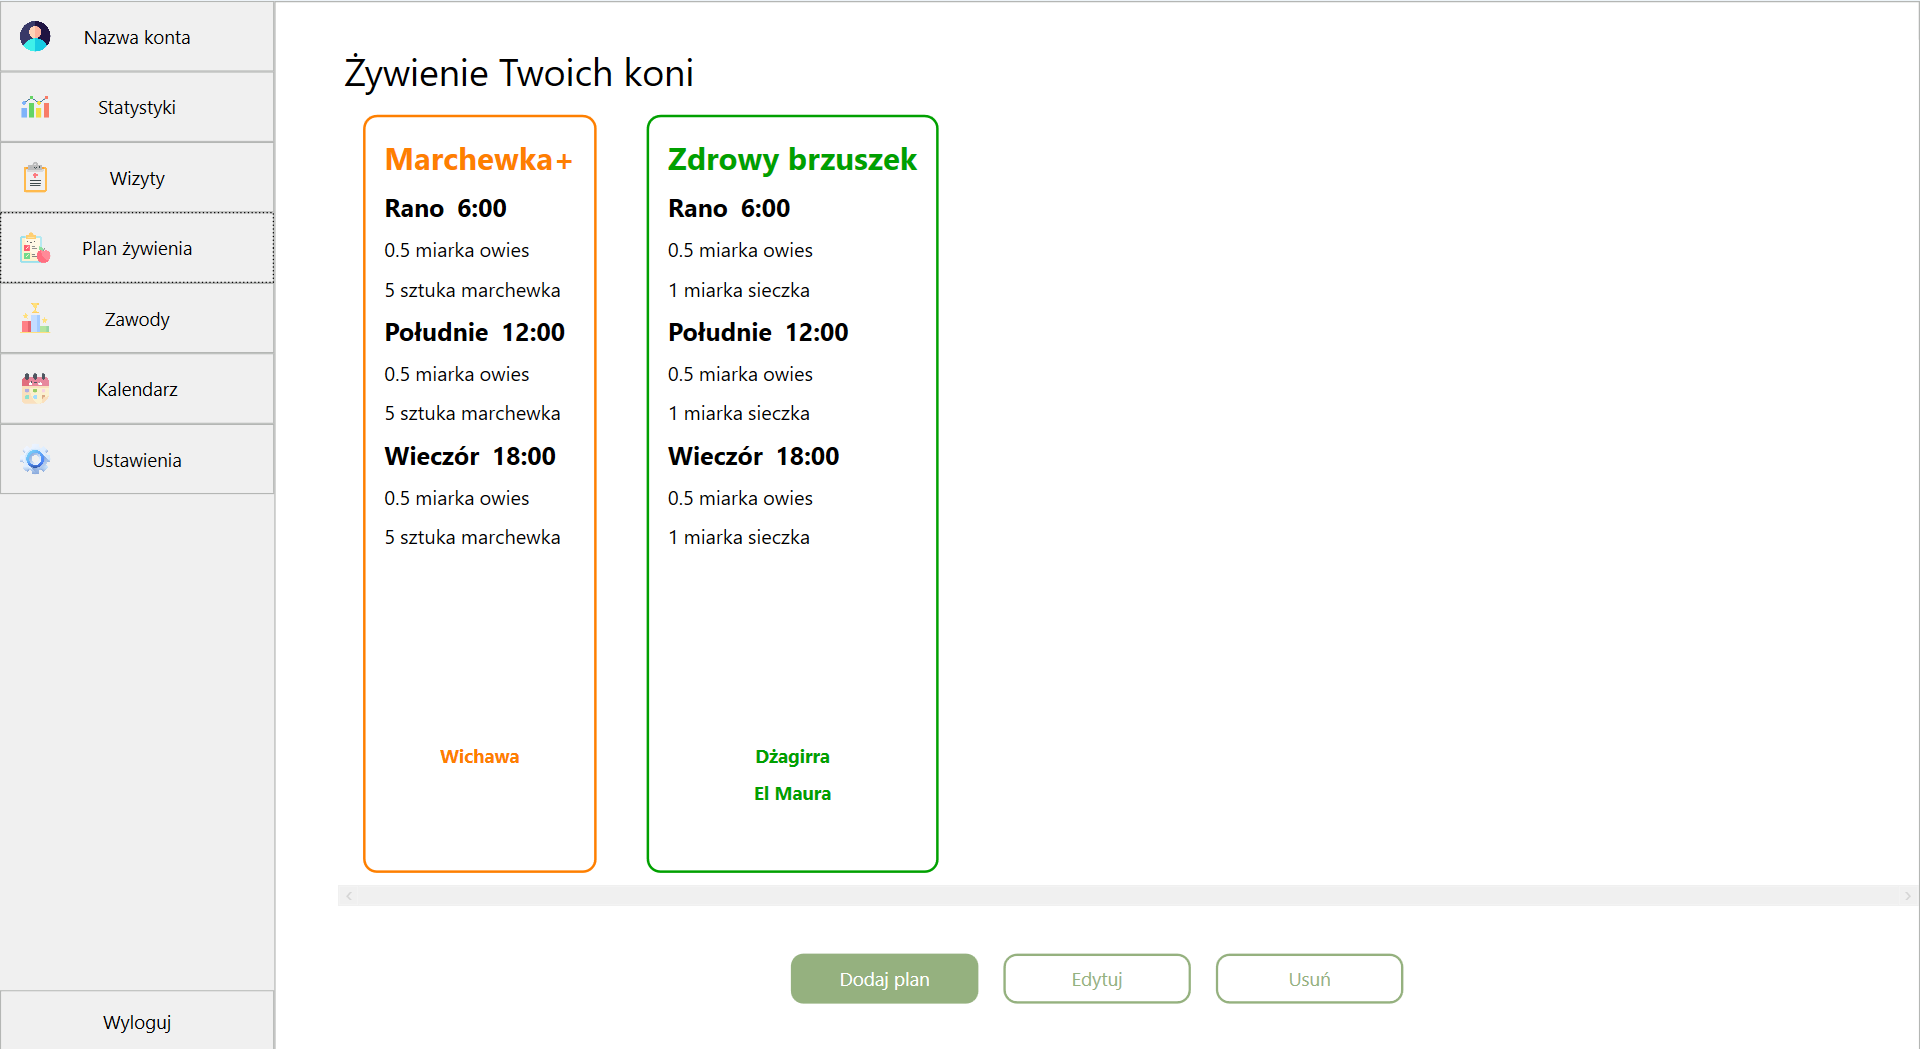
\includegraphics[scale=0.4]{Zywienie}
	\caption{Strona żywienia}
	\textit{Źródło: Opracowanie własne}
	\label{Zywienie}
\end{figure}

Na menu bocznym dostępna jest także zakładka "Żywienie" pozwalająca na zarządzanie planami żywienia. Po kliknięciu zostajemy przeniesieni na stronę widoczną na rysunku \ref{Zywienie}. Dla każdego z koni można ustawić jego indywidualny plan, poprzez kliknięcie przycisku ,,dodaj plan''. Jest on całkowicie modyfikowalny, może zawierać dowolną ilość posiłków podawanych o dowolnej porze dnia, każdy posiłek może zawierać wiele składników w różnych ilościach. \textcolor{red}{Pory posiłków oraz ich nazwy można ustawić po kliknięciu przycisku ustawienia. W tym miejscu można także dodać nowe rodzaje składników posiłku takich jak pasze, warzywa itp..} Wiele koni może być aktualnie na tej samej diecie i stosować ten sam plan żywienia. Na dole planu wypisane są imiona koni, które aktualnie są na tej diecie co pozwala na łatwą identyfikację. Każdy z planów ma swój kolor dzięki czemu użytkownik od razu wie na który plan spojrzeć. Pory posiłków zostały napisane wytłuszczoną czcionką, co poprawienia czytelności. Na tej stronie można zapisać dowolnie wiele planów żywienia, nie każdy z nich musi być obecnie używany. Jeśli zostanie zapisane więcej danych niż może zmieścić ekran pojawią się suwaki dzięki, którym można obserwować wszystkie zapisane informacje.

Jak zostało wcześniej wspomniane, aby dodać kolejne plany należy kliknąć przycisk "dodaj plan". Kliknięcie go powoduje otwarcie nowego okna widocznego na rysunku \ref{DodajZywienie}. W oknie tym możemy nadać tytuł naszemu planu wybrać kolor, dodać opis oraz stworzyć plan poprzez dodawanie kolejnych składników oraz posiłków.  Każdy wybrany przez nas składnik musi podawany być w odpowiedniej ilości, aby konie zdrowo się odżywiały w tym celu przy każdej paszy którą mamy do wyboru dostępne jest pole do wpisania ilości oraz miejsce w którym możemy wybrać w jakiej miarze została podana ilość. 

Możliwa jest także późniejsza edycja planów poprzez kliknięcie przycisku edytuj na stronie głównej. W tym przypadku otwiera się to samo okno co przy dodawaniu planu jednakże jest ono już uzupełnione danymi (patrz. rys \ref{EdytujZywienie}). Po dodaniu bądź edycji planu użytkownik zostanie przekierowany na stronę główną. Jeśli dodany plan go nie satysfakcjonuje można go usunąć klikając przycisk usuń.

\begin{figure} [H]
	\begin{center}
		\begin{minipage}{6cm}
			\centering
			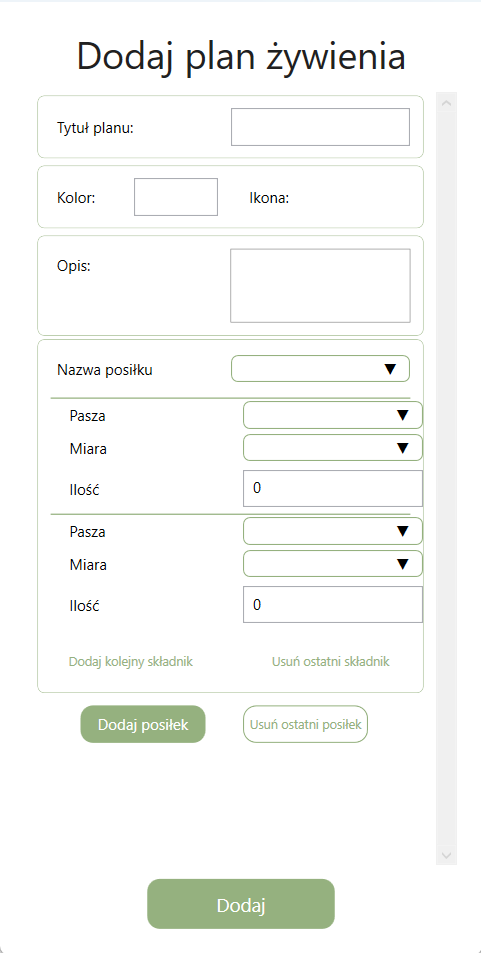
\includegraphics[scale=0.7]{dodajZywienie}
			\caption{Dodawanie żywienia}
			\textit{Źródło: Opracowanie własne}
			\label{DodajZywienie}
		\end{minipage}
		\hfil
		\begin{minipage}{6cm}
			\centering
			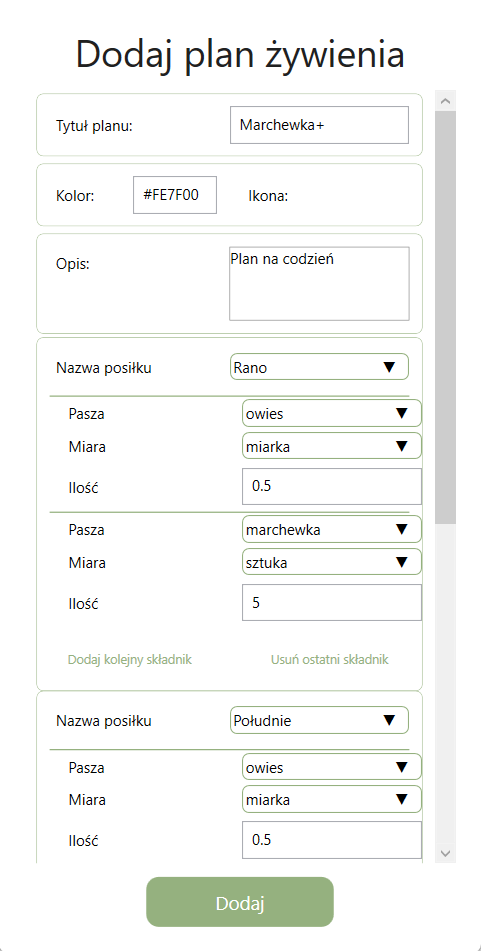
\includegraphics[scale=0.7]{edytujZywienie}
			\caption{Edycja żywienia}
			\textit{Źródło: Opracowanie własne}
			\label{EdytujZywienie}
		\end{minipage}
	\end{center}
\end{figure}

Na menu bocznym dostępną mamy także zakładkę zawody. Po kliknięciu w nią użytkownik przeniesiony zostanie na stronę gdzie możliwe jest zarządzanie zawodami. Po wejściu widzimy listę zawodów oraz puste miejsce po prawej stronie. Kliknięciu w dowolne zawody dostępne na liście spowoduje pojawienie się po prawej stronie od listy, spisu konkursów dostępnych na tych zawodach. Jeśli jakiś koń jest już zapisany na te zawody jego imię pojawi się pod każdym z konkursów w których bierze udział. Jeśli zawody są już zakończone wyniki konia będą uzupełnione. 
\begin{figure}[h]
\centering
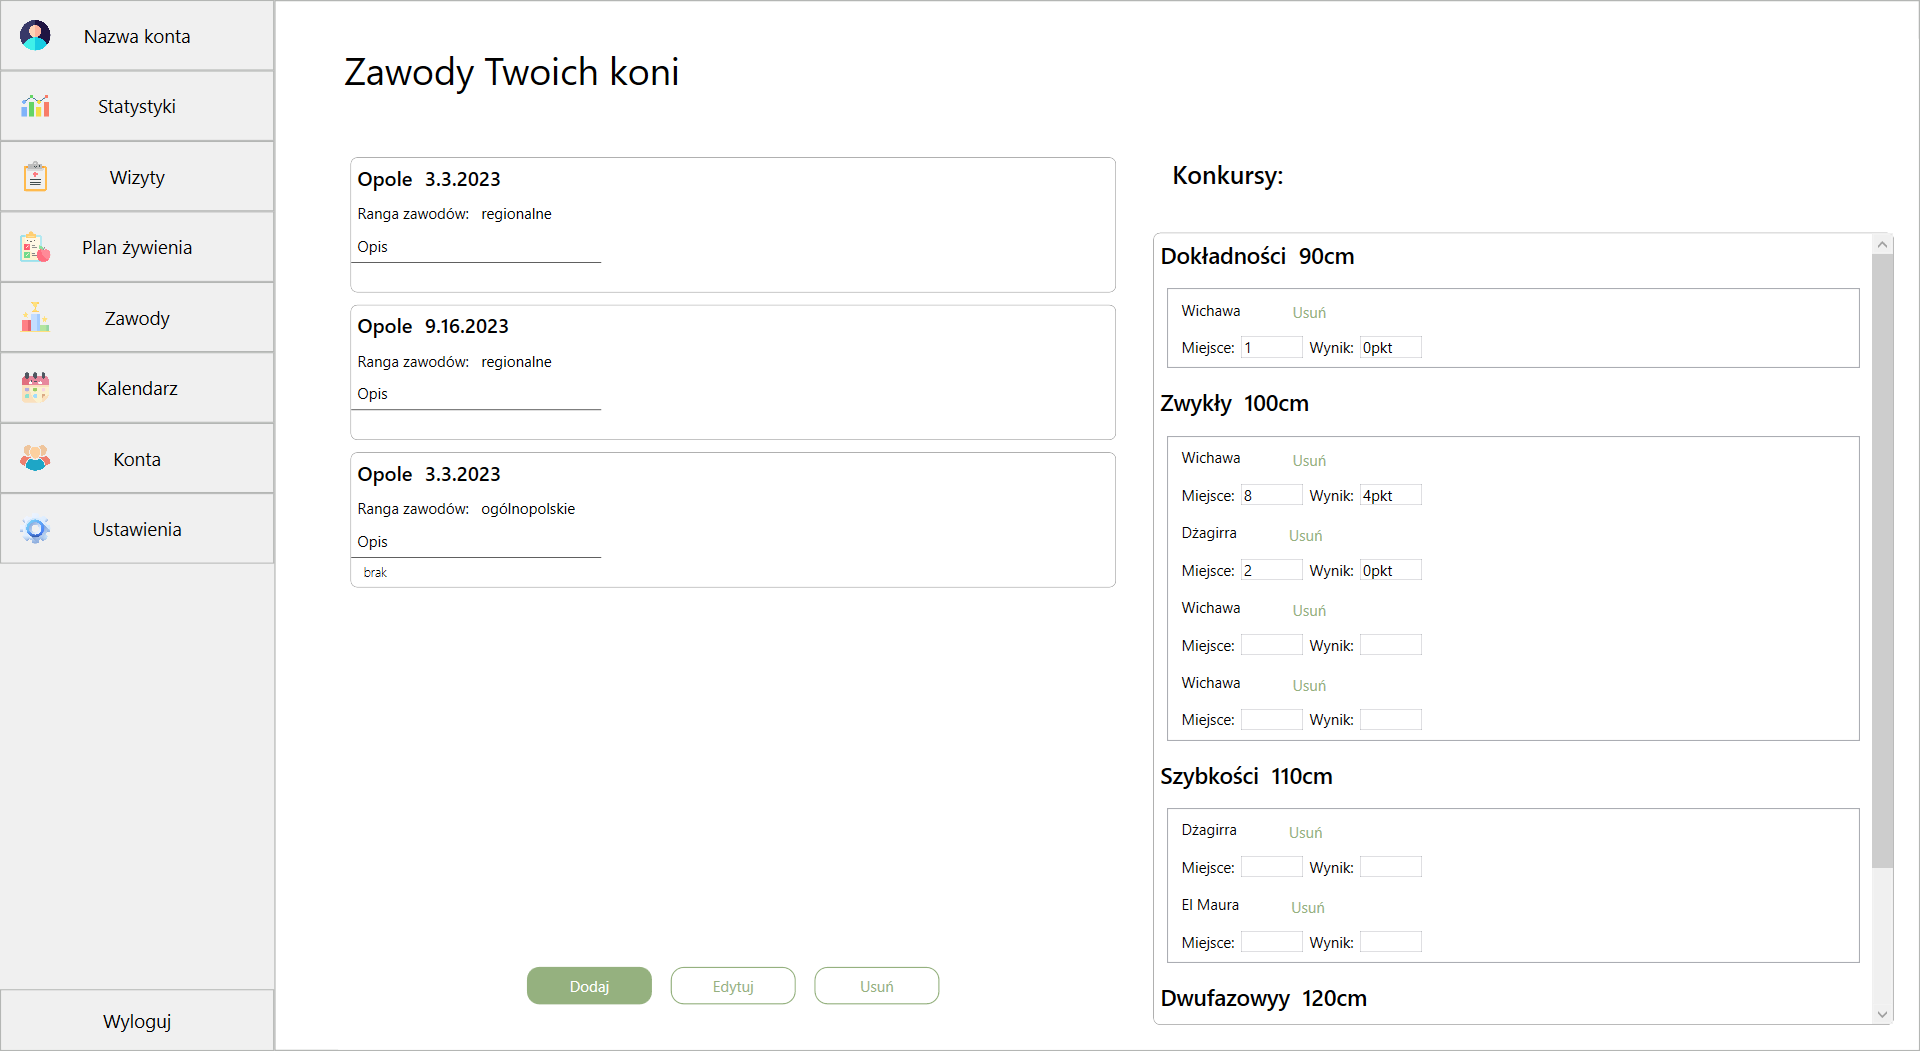
\includegraphics[scale=0.4]{zawody}
\caption{Strona zawodów}
\textit{Źródło: Opracowanie własne}
\label{StronaZawodow}
\end{figure}
Aby dodać nowego konia do zawodów należy kliknąć w nazwę konkursu. Poskutkuje to otwarciem nowego okna z wyborem konia, którego chcemy dodać. Po zakończonych zawodach możemy dodać wyniki naszego konia uzupełniając odpowiednie pola. Możemy także usunąć start konia w zawodach klikając przycisk usuń.



{\color{red} Ustawienia, Zarządzanie kontami, kalendarz}
\newpage
\section{Aplikacja mobilna}
Aplikacja mobilna "HorseTracking" służy do zapisywania dziennych aktywności koni, ich wizyt u lekarzy, kowali jak także do zarządzania zawodami.

\begin{wrapfigure}{r}{0.5\linewidth}
	\centering
	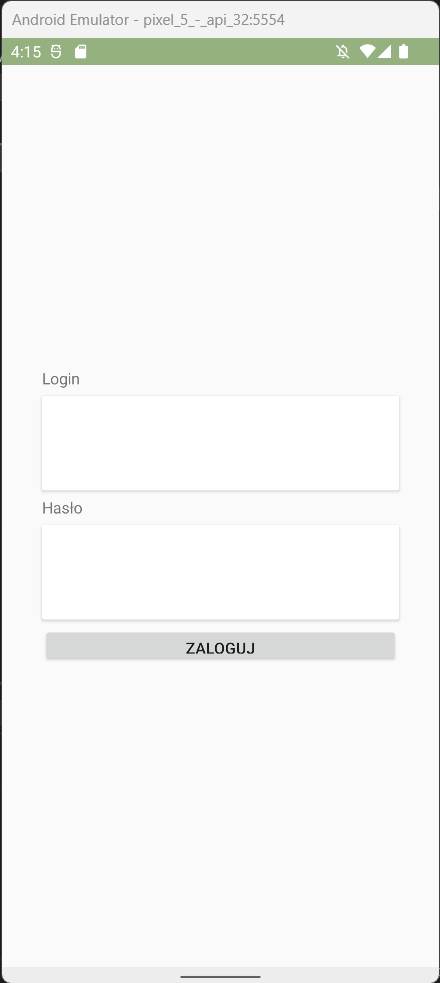
\includegraphics[scale=0.35]{LoginView}
	\caption{\centering Logowanie do aplikacji.}
	\textit{\centering Źródło: Opracowanie własne}
	\label{LoginView}
	\newline
	\newline
		\centering
	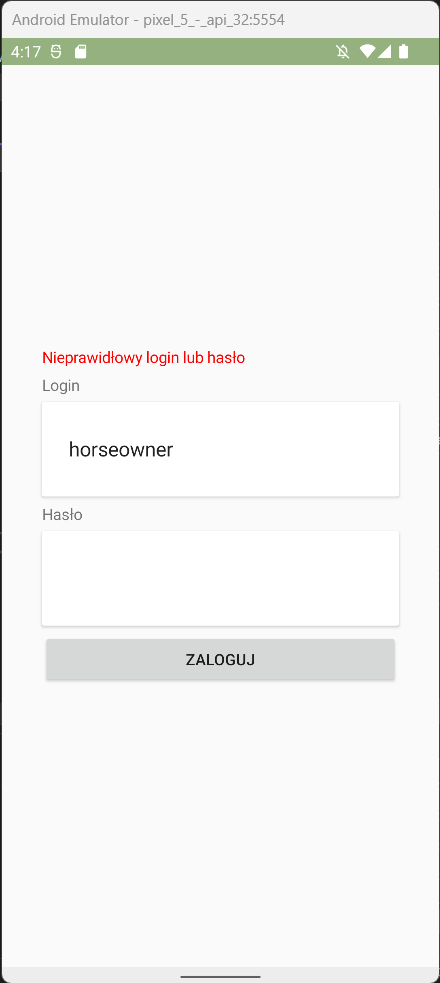
\includegraphics[scale=0.35]{WrongLoginData}
	\caption{\centering Błędne dane logowania.}
	\textit{\centering Źródło: Opracowanie własne}
	\label{LoginViewWrongPassword}
\end{wrapfigure}
Po pierwszym otwarciu aplikacji użytkownikowi ukaże się okno logowania przedstawione na rysunku \ref{LoginView}. 

Na tym ekranie użytkownik może zalogować się do aplikacji. \textcolor{red}{Możliwa jest także opcja zresetowania swojego hasła, w przypadku zapomnienia hasła}. Rejestracja do aplikacji nie jest możliwa, ponieważ ta funkcja jest dostępna jedynie dla administratora w aplikacji desktopowej. Po wprowadzeniu loginu i hasła, a następnie kliknięciu przycisku "Zaloguj" sprawdzana jest poprawność wprowadzonych danych. 

Jeśli przy próbie zalogowania podane zostaną nieprawidłowe dane logowania, bądź użytkownika nie ma w systemie, zostanie on o tym poinformowany (patrz. rys \ref{LoginViewWrongPassword})
Użytkownik nieposiadający koni (użytkownik typu appOwner) nie może zalogować się do aplikacji mobilnej, ponieważ służy ona tylko do wpisywania danych o swoich koniach.

Po poprawnym zalogowaniu się dane użytkownika zostają zapamiętane, więc przy kolejnym otwarciu aplikacji użytkownik będzie już zalogowany.
Aby wylogować się z aplikacji użytkownik musi otworzyć menu boczne i wybrać opcję "Wyloguj".

\begin{wrapfigure}{r}{0.59\textwidth}
	\centering
	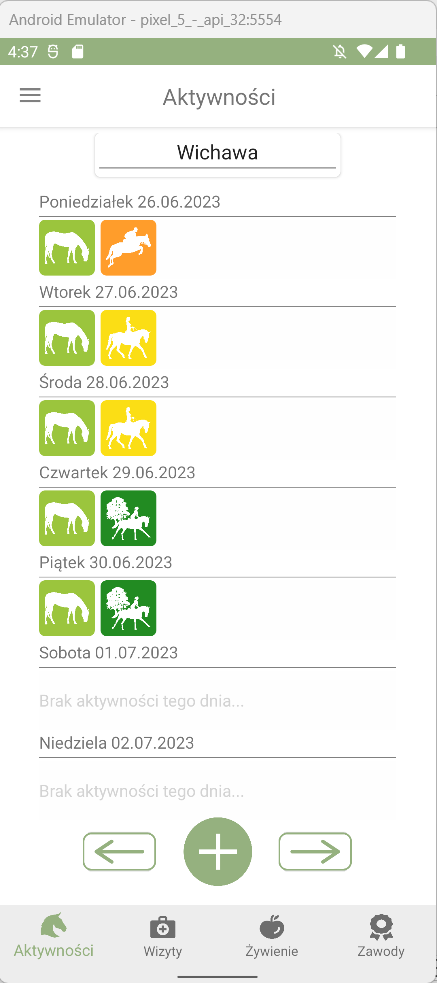
\includegraphics[scale=0.8]{ActivityView}
	\caption{Ekran aktywności.}
	\textit{Źródło: Opracowanie własne}
	\label{ActivityView}
\end{wrapfigure} 

Po zalogowaniu do aplikacji użytkownik zostaje przeniesiony na okno główne. Zawiera ono menu dolne pozwalające na nawigację pomiędzy czterema głównymi sekcjami aplikacji: aktywności, wizyty, żywienie, zawody. Na początek wyświetlona zostaje  strona dotycząca aktywności. W tym widoku można przeglądać informacje o wszystkich aktywnościach koni posiadanych lub tych które trenujemy.  

Aktywności dotyczą konia, którego imię podane jest w polu powyżej. Aby zmienić konia wystarczy kliknąć w to pole i wybrać innego konia.
Strzałki lewo-prawo widoczne na dole ekranu umożliwiają nawigację między kolejnymi tygodniami. W przypadku braku aktywności w danym dniu, wyświetlony jest napis informujący o braku aktywności tego dnia. Każdy typ aktywności ma inny kolor i ikonę, aby ułatwić identyfikacje. Po kliknięciu w daną aktywność możemy przejść do detali dotyczących tej aktywności. Ekran szczegółów został przedstawiony na rysunku \ref{ActivityDetails} i zostanie omówiony później.

Pomiędzy strzałkami nawigującymi miedzy tygodniami znajduje się okrągły przycisk z ikoną "+". Umożliwia on dodawanie aktywności. Dla aktualnie wybranego konia. Przycisk ten dostępny jest jedynie dla właściciela konia oraz osób którym dany koń został udostępniony. Oznacza to, że jeśli użytkownik jest trenerem ta opcja jest dla niego zablokowana, a przycisk nie jest widoczny.

Po kliknięciu w przycisk "+" użytkownik zostaje przeniesiony na okno "Dodawanie aktywności".
\begin{figure}[H]
	\begin{center}
	\begin{minipage}{5cm}
	\centering
	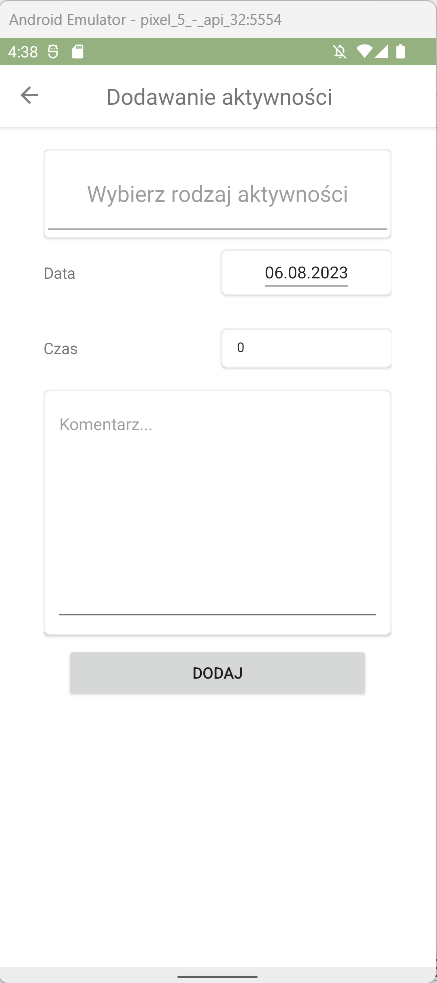
\includegraphics[scale=0.6]{AddActivitySimpleView}
	\caption{\centering Okno dodawania aktywności.}
	\textit{Źródło: Opracowanie własne}
	\label{AddActivitySimple}
\end{minipage}
\hfil
\begin{minipage}{5cm}
	\centering
	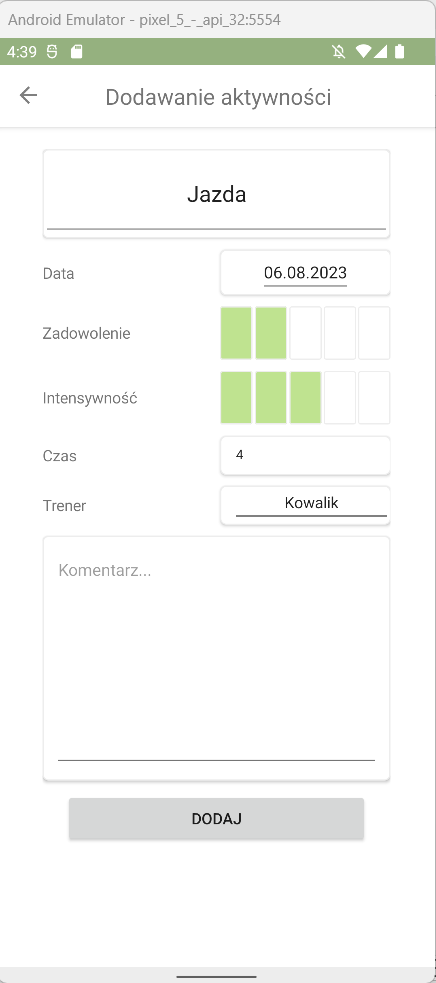
\includegraphics[scale=0.6]{AddActivityAdvancedView}
	\caption{Okno dodawania aktywności rozszerzone.}
	\textit{Źródło: Opracowanie własne}
	\label{AddActivityAdvanced}
\end{minipage}
	\end{center}
\end{figure}
Okno to wygląda różnie w zależności od tego jaki typ aktywności chcemy dodać (patrz rys. \ref{AddActivitySimple} i rys. \ref{AddActivityAdvanced}). Na początku wyświetlony jest prostszy model okna, a po wybraniu typu aktywności dostosowuje się. Dla aktywności: jazda, skoki, zawody, kros czy skoki w oknie dochodzą nowe opcje takie jak satysfakcja, intensywność oraz wybór trenera (patrz. rys \ref{AddActivityAdvanced}). Po uzupełnieniu wszystkich niezbędnych informacji aktywność zostaje dodana i pojawia się na ekranie głównym. Jeśli któraś z niezbędnych informacji nie zostanie uzupełniona aktywność nie doda się, użytkownik zostanie poinformowany o nieprawidłowościach i będzie mógł je poprawić.
\begin{wrapfigure}{r}{0.6\textwidth}
	\centering
	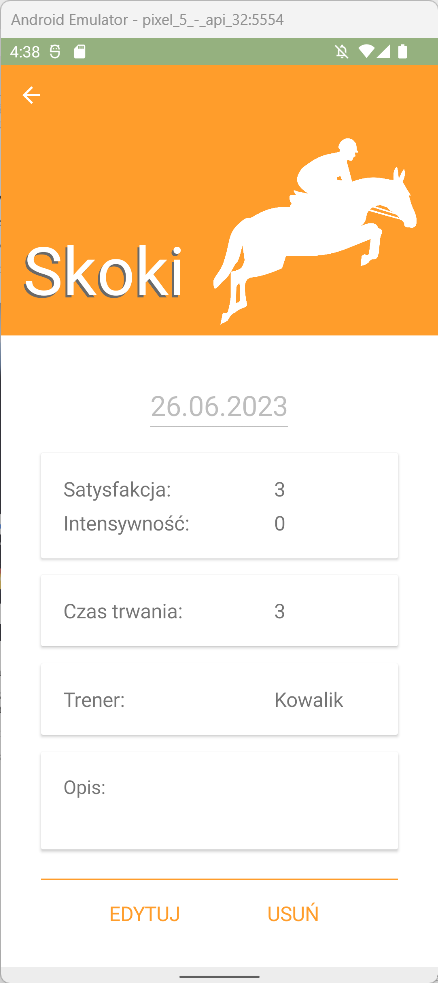
\includegraphics[scale=0.7]{ActivityDetailsView}
	\caption{\centering Szczegóły aktywności.}
	\textit{Źródło: Opracowanie własne}
	\label{ActivityDetails}
\end{wrapfigure}
Po dodaniu aktywności użytkownik zostaje przeniesiony z powrotem na okno główne, gdzie po kliknięciu w wybraną aktywność może zobaczyć jej szczegóły (patrz rys.\ref{ActivityDetails} ). 

W oknie szczegółów oprócz przeczytania wszystkich informacji dotyczących aktywności można także przejść do edycji lub usunąć daną aktywność. Przy edycji otwiera się to samo okno co przy dodawaniu aktywności jednakże tym razem jest ono wypełnione aktualnymi danymi wybranej aktywności. Po zakończonej edycji użytkownik zostaje przeniesiony na okno główne. Po kliknięciu przycisku usuń, wyświetla się komunikat proszący o potwierdzenie wykonania akcji. Jeśli użytkownik potwierdzi, że akcje, to aktywność zostanie usunięta, a użytkownik zostanie przeniesiony na ekran główny. \textcolor{red}{Usunięcie aktywności jest także możliwe poprzez długie przytrzymanie wybranej aktywności na ekranie głównym, a następnie potwierdzenie akcji na pojawiającym się komunikacie.}
\newpage
Kolejną opcją w menu dolnym są wizyty. Na tym oknie podobnie jak w oknie aktywności mamy pole pozwalające wybrać konia o którym informacje chcemy obejrzeć. Koń wybrany na oknie aktywności przenosi się na okno wizyt i na odwrót. W tym oknie można sprawdzić jakie wizyty odbył ostatnio wybrany koń. 
\begin{figure}[H]
	\begin{center}
	\begin{minipage}{5cm}
		\centering
		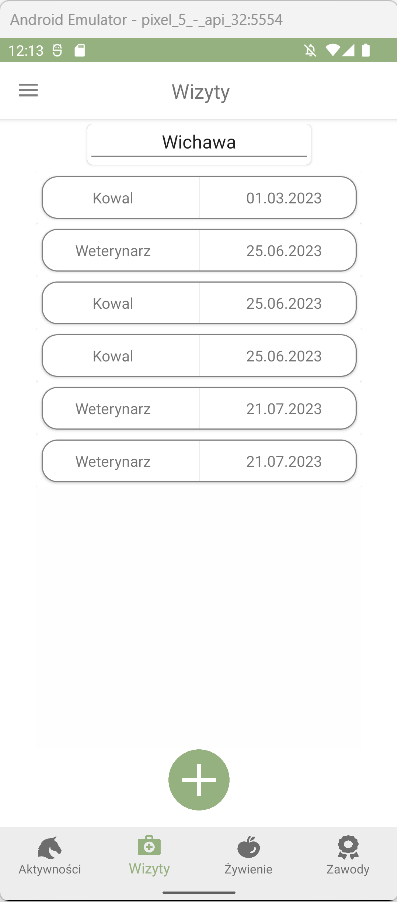
\includegraphics[scale=0.6]{VisitView}
		\caption{\centering Okno wizyt.}
		\textit{Źródło: Opracowanie własne}
		\label{VisitView}
	\end{minipage}
	\hfil
	\begin{minipage}{5cm}
		\centering
		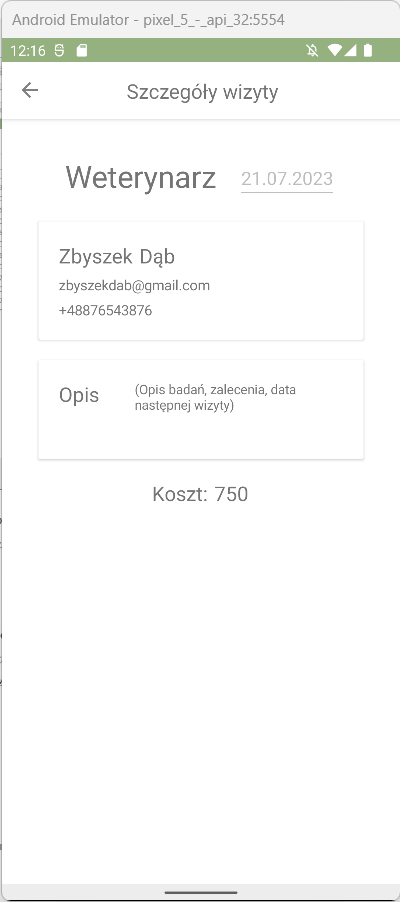
\includegraphics[scale=0.6]{VisitViewDetails}
		\caption{\centering Szczegóły wizyty.}
		\textit{Źródło: Opracowanie własne}
		\label{VisitDetailsView}
	\end{minipage}
\end{center}
\end{figure}
Na rysunku \ref{VisitView} widzimy listę wizyt wybranego konia. Po kliknięciu w wizytę zostaniemy przeniesieni do szczegółów wizyty, gdzie możemy znaleźć dane kontaktowe do lekarza/kowala, który przeprowadził wizytę oraz szczegóły takie jak opis wizyty i jej koszt. Dzięki temu widokowi użytkownik może sprawdzić jakie zalecenia były na poprzednich wizytach, jaki był ich koszt i kiedy dokładnie się odbyły.
\newpage
\begin{wrapfigure}{r}{0.6\textwidth}
	\centering
	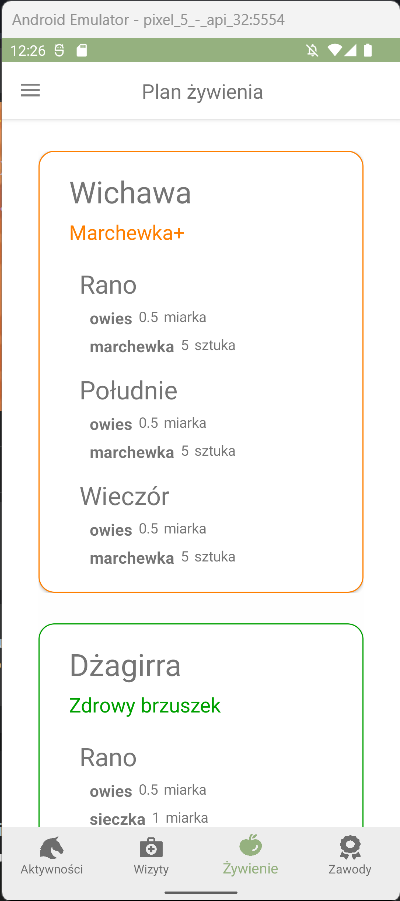
\includegraphics[scale=0.7]{NutritionPlan}
	\caption{\centering Plany żywienia.}
	\textit{Źródło: Opracowanie własne}
	\label{NutritionPlan}
\end{wrapfigure}
Kolejną opcją dostępną w menu dolnym są plany żywienia. Po kliknięciu w ikonę jabłka użytkownik zostanie przeniesiony na stronę z planami żywienia wszystkich jego koni. Plany żywienia przedstawione zostały na liście, którą możemy scrollować, aby zobaczyć wszystkie plany dotyczące naszych koni. W widoku tym można jedynie obejrzeć plany żywienia (patrz \ref{NutritionPlan}), nie jest możliwe ich dodanie, edycja bądź usunięcie. Całość zarządzania planami żywienia została zaimplementowana w aplikacji desktopowej. Dzięki tej zakładce użytkownicy przebywający w stajni mogą sprawdzić dietę konia i przygotować dla niego posiłki. Plany zostały przedstawione w przejrzysty sposób, gwarantujący możliwość szybkiego sprawdzenia diety konia. Kolory oraz tytuły zastosowane w poszczególnych planach są ściśle z nimi związane i można je ustalić przy tworzeniu planu, dzięki nim po jednym spojrzeniu wiemy, który plan dotyczy którego konia. 

Ostatnia zakładka dostępna w menu dolnym z ikoną nagrody "flo" rozety rozdawanej na zawodach, przenosi nas do strony, na której możemy obejrzeć informacje dotyczące zawodów. Na tej stronie widzimy listę startów naszych koni w różnych zawodach. Starty te zostały posegregowane według daty od najwcześniejszego do najbardziej odległego w czasie. Jeśli zawody już się zakończyły i uzupełnione zostały wyniki z tych zawodów to one także pojawią się na tej liście. Okno zawodów można zobaczyć na rysunku \ref{Competition}.
\begin{figure}[H]
	\centering
	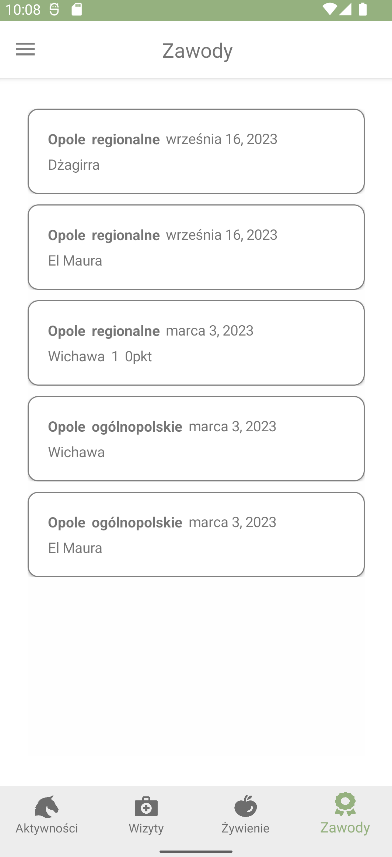
\includegraphics[scale=0.7]{CompetitionView}
	\caption{\centering Okno przedstawiające starty w zawodach.}
	\textit{Źródło: Opracowanie własne}
	\label{Competition}
\end{figure}

W aplikacji mobilnej oprócz menu dolnego, które prowadzi nas przez najważniejsze funkcjonalności aplikacji mamy także menu boczne. W menu bocznym mamy możliwość wylogowania się z aplikacji. Wyjście z aplikacji nie powoduje wylogowania, użytkownik po wpisaniu swoich danych zostaje zapamiętany i po wejściu do aplikacji będzie już zalogowany na swoje konto. Dlatego w menu bocznym dodany został przycisk powodujący wylogowanie, dzięki czemu inna osoba może zalogować się na swoje konto. Oprócz tego w menu bocznym znajduję się przycisk pozwalający na przejście do panelu udostępniania (patrz rys. \ref{Share}).
\begin{figure}[H]
	\centering
	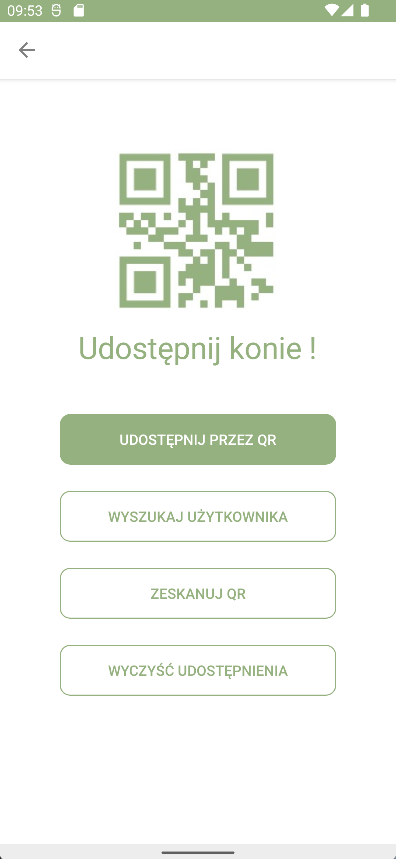
\includegraphics[scale=0.7]{ShareView}
	\caption{\centering Panel udostępniania.}
	\textit{Źródło: Opracowanie własne}
	\label{Share}
\end{figure}

 W tym miejscu można przejść do udostępniania przez kod QR. Gdzie po wybraniu konia do udostępnienia oraz daty do której ma być udostępniony możemy wygenerować kod QR (patrz rys. \ref{ShareQR}). Dzięki któremu inna osoba posiadająca aplikację będzie mogła go zeskanować i dodać do swojej puli koni. Można także udostępnić konia danemu użytkownikowi poprzez wyszukanie go na liście wszystkich użytkowników (patrz rys. \ref{ShareSearch}). Po udostępnieniu koń znika z listy koni właściciela, powróci na nią dopiero po zakończeniu daty udostępniania, bądź po kliknięciu przycisku "Usuń udostępnienia". Osoba która dostała konia nie może go usunąć samodzielnie ze swojej listy. 
\begin{figure}[H]
	\begin{center}
		\begin{minipage}{5cm}
			\centering
			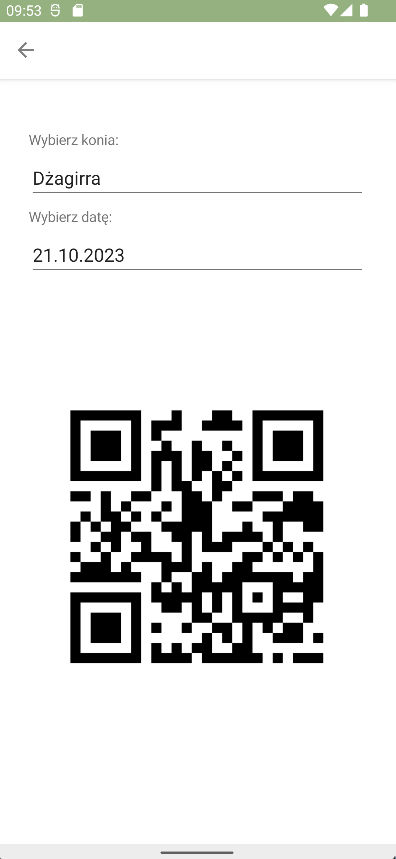
\includegraphics[scale=0.6]{ShareQR}
			\caption{\centering Udostępnianie koni przez QR.}
			\textit{Źródło: Opracowanie własne}
			\label{ShareQR}
		\end{minipage}
		\hfil
		\begin{minipage}{5cm}
			\centering
			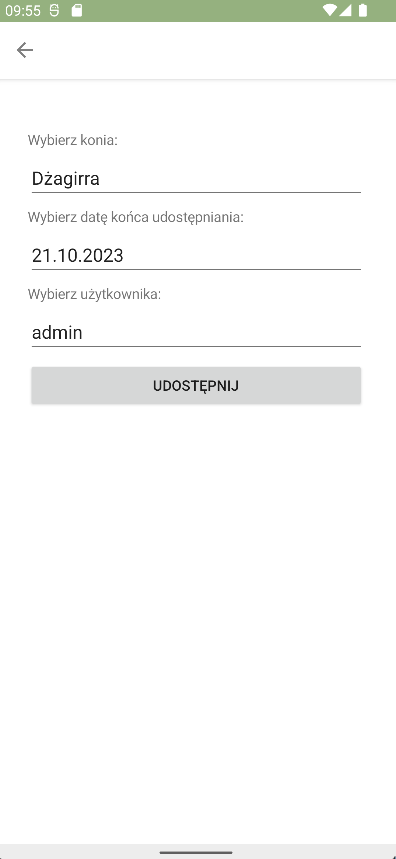
\includegraphics[scale=0.6]{SharebySearch}
			\caption{\centering Udostępnianie koni przez wyszukiwarkę.}
			\textit{Źródło: Opracowanie własne}
			\label{ShareSearch}
		\end{minipage}
	\end{center}

\end{figure}
\chapter{Podsumowanie}
\begin{thebibliography}{9}
	
	\bibitem{bazydanych}
	Hanna Mazur, Zygmunt Mazur,
	\emph{Projektowanie relacyjnych baz danych}.
	Oficyna Wydawnicza Politechniki Wrocławskiej, Wrocław 2004.

	\bibitem{XamarinLearn} profexorgeek, alexbuckgit, v-hearya, davidbritch, conceptdev \emph{Co to jest środowisko Xamarin?}
	https://learn.microsoft.com/pl-pl/xamarin/get-started/what-is-xamarin [Dostęp: 06.08.2023] 

	\bibitem{Nuget} JonDouglas, alexbuckgit, Mikejo5000, v-hearya, zivkan, chrisraygill, loic-sharma, karann-msft, NickKruger,	mairaw, kraigb, alfredmyers, \emph{Wprowadzenie do narzędzia NuGet} https://learn.microsoft.com/pl-pl/nuget/what-is-nuget 
	[Dostęp: 06.08.2023]

	\bibitem{Entity}Paweł Łukasiewicz \emph{C\# - Entity Framework} https://www.plukasiewicz.net/Artykuly/EntityFramework
	[Dostęp: 06.08.2023]

	\bibitem{FigmaBlog} Juris Lavrinovics, \emph{Figma - narzędzie do projektowania interfejsu użytkownika}
	https://blog.consdata.tech/2023/02/15/uiux-tools.html 
	[Dostęp 05.05.2023]

	\bibitem{FigmaAbout}https://www.figma.com/about/ 
	[Dostęp 05.05.2023]

	\bibitem{FigmaIcon}Figma \emph{Figma-logo} https://commons.wikimedia.org/wiki/File:Figma-logo.svg 
	[Dostęp 05.05.2023]
	
	\bibitem{WPF} adegeo, ihsansfd, alexbuckgit, v-trisshores, DCtheGeek, \emph{Przewodnik dotyczący aplikacji klasycznych (WPF .NET)}\\ https://learn.microsoft.com/pl-pl/dotnet/desktop/wpf/overview/?view=netdesktop-7.0 
	[Dostęp: 06.08.2023]
	
	\bibitem{bazadanychFizyczny}  Sharon Allen, Evan Terry, \emph{Beginning Relational Data Modeling}, Apress Berkeley, CA, 2005
	
	\bibitem{git} GIT \emph{Git --local-branching-on-the-cheap} https://git-scm.com/ [Dostęp 10.10.2023]
	
	\bibitem{github} GitHub - https://github.com/ [Dostęp 10.10.2023]
	
	\bibitem{sourcetree} Sourcetree - https://www.sourcetreeapp.com/ [Dostęp 10.10.2023]
	
	\bibitem{mvvmpattern} MVVM Pattern https://en.wikipedia.org/wiki/Model-view-viewmodel [Dostęp 12.10.2023]
	
	\bibitem{MVVMmicLearn} davidbritch, nschonni, conceptdev, JohnCOsborne \emph{The Model-View-ViewModel Pattern} https://learn.microsoft.com/en-us/xamarin/xamarin-forms/enterprise-application-patterns/mvvm
	[Dostęp 14.10.2023]
	
	\bibitem{DI} Michał Miszczyszyn \emph{Wzorce Projektowe: Dependency Injection} https://typeofweb.com/wzorce-projektowe-dependency-injection
	[Dostęp 14.10.2023]
	
	\bibitem{EntityFramework} Microsoft Learn \emph{Dokumentacja EnitiyFramework} https://learn.microsoft.com/pl-pl/ef/
	[Dostęp 14.10.2023]
\end{thebibliography}
\listoffigures
\lstlistoflistings
\listoftables
\chapter*{Opis zawartości APD}


\end{document}